% **************************************************************************************************************
% A Classic Thesis Style
% An Homage to The Elements of Typographic Style
%
% Copyright (C) 2011 Andr\'e Miede http://www.miede.de
%
% If you like the style then I would appreciate a postcard. My address 
% can be found in the file ClassicThesis.pdf. A collection of the 
% postcards I received so far is available online at 
% http://postcards.miede.de
%
% License:
% This program is free software; you can redistribute it and/or modify
% it under the terms of the GNU General Public License as published by
% the Free Software Foundation; either version 2 of the License, or
% (at your option) any later version.
%
% This program is distributed in the hope that it will be useful,
% but WITHOUT ANY WARRANTY; without even the implied warranty of
% MERCHANTABILITY or FITNESS FOR A PARTICULAR PURPOSE.  See the
% GNU General Public License for more details.
%
% You should have received a copy of the GNU General Public License
% along with this program; see the file COPYING.  If not, write to
% the Free Software Foundation, Inc., 59 Temple Place - Suite 330,
% Boston, MA 02111-1307, USA.
%
% **************************************************************************************************************
% Note:
%    * You must not use "u etc. in strings/commands that will be spaced out (use \"u or real umlauts instead)
%    * New enumeration (small caps): \begin{aenumerate} \end{aenumerate}
%    * For margin notes: \marginpar or \graffito{}
%    * Do not use bold fonts in this style, it is designed around them
%    * Use tables as in the examples
%    * See classicthesis-preamble.sty for useful commands
% **************************************************************************************************************
% To Do:
%		 * [high] Check this out: http://www.golatex.de/koma-script-warnung-in-verbindung-mit-listings-package-t2058.html
%    * [medium] mathbb in section-titles/chapter-titles => disappears somehow in headlines!!!
% **************************************************************************************************************
\documentclass[ oneside,openright,titlepage,numbers=noenddot,headinclude,%1headlines,% letterpaper a4paper
                footinclude=false,cleardoublepage=empty,abstractoff, % <--- obsolete, remove (todo)
                BCOR=5mm,paper=a4,fontsize=11pt,%11pt,a4paper,%
                ngerman,american,%
                ]{scrreprt}

%********************************************************************
% Note: Make all your adjustments in here
%*******************************************************
\usepackage{Style/classicthesis-preamble} % [backref]
\usepackage[left=40mm,right=25mm,top=20mm,bottom=40mm]{geometry}
\usepackage{natbib}
\usepackage{amsfonts}
\usepackage{type1cm} % scalable fonts
\usepackage{lettrine}
\usepackage{breqn}
\usepackage{graphicx}
\usepackage{amsthm}
\usepackage{algpseudocode}
\usepackage{algorithm}
\usepackage{tikz}
\usepackage{tabularx}
\usetikzlibrary{chains,fit,shapes, matrix}
\usepackage{enumitem} 
\SetLabelAlign{parright}{\parbox[t]{\labelwidth}{\raggedright#1}}
\setlist[description]{style=multiline,leftmargin=3cm, align=parright,itemsep=2mm}
%\usepackage{caption}
%\usepackage{subcaption}
\makeatletter
\renewcommand\bibsection{\section*{}}
\makeatother
\usepackage{multibib}
\newcites{own}{Publications}
\newcites{others}{Bibliography}
\newtheorem{mydef}{Definition}
\newtheorem{ex}{Example}
\usepackage{xcolor}
\usepackage{adjustbox}
\DeclareMathOperator*{\argmin}{arg\,min}
\newenvironment{myexample}[1]
{\begin{adjustbox}{minipage=[b]{380px},margin=1ex,bgcolor=gray!10,env=center}\begin{ex}#1\end{ex}}
{\end{adjustbox}}
\newtheorem{thm}{Theorem}[section]
\newenvironment{mytheorem}[1]
{\begin{thm}#1\end{thm}}
{}
\newtheorem{corollary}{Corollary}
\newtheorem{lemma}{Lemma}
\newtheorem{ratio_lemma}{Lemma}
%\renewcommand\baselinestretch{1}
\usepackage{setspace}
\doublespacing
\usepackage{color}
\newcommand{\ToDo}[1]{\textbf{\large\textcolor{blue}{[#1]}}}
%*******************************************************
% Some font experiments
%*******************************************************
%\usepackage[osf]{libertine}
%\usepackage{hfoldsty}
%\usepackage[light,condensed,math]{iwona}
%\renewcommand{\sfdefault}{iwona}
%\usepackage{lmodern} % <-- no osf support :-(
%\usepackage[urw-garamond]{mathdesign} <-- no osf support :-(

%*******************************************************
% Fine-tuning for the text area
%*******************************************************
%\linespread{1.05} % a bit more for Palatino
%\areaset[current]{312pt}{761pt} % 686 (factor 2.2) + 33 head + 42 head \the\footskip
%\setlength{\marginparwidth}{7em}%
%\setlength{\marginparsep}{2em}%

%********************************************************************
% Hyphenation
%*******************************************************
%\hyphenation{put special hyphenation here}

% ********************************************************************
% GO!GO!GO! MOVE IT!
%*******************************************************

\usepackage{breqn}
\newenvironment{myMaths}{\footnotesize \begin{dmath}}{\end{dmath}}
\setlength{\headheight}{25pt}
\addtolength{\jot}{1em} % space between aligned equations
\newcommand{\logTerm}[2]{#1\overline{\log} #1 + #2\overline{\log} #2 - (#1+#2)\overline{\log}(#1+#2)}
\newcommand{\G}{\mathcal{G}}
\newcommand{\D}{\mathcal{D}}
\newcommand{\C}{\mathbb{C}}
\newcommand{\K}{\mathbb{K}}
\newcommand{\N}{\mathbb{N}}
\newcommand{\p}{\mathcal{P}}
\newcommand{\F}{\mathcal{F}}

\begin{document}
\frenchspacing
\raggedbottom
\selectlanguage{american} % american ngerman
%\renewcommand*{\bibname}{new name}
%\setbibpreamble{}
\pagenumbering{roman}
\pagestyle{plain}
%********************************************************************
% Frontmatter
%*******************************************************
%*******************************************************
% Titlepage
%*******************************************************
\begin{titlepage}
	% if you want the titlepage to be centered, uncomment and fine-tune the line below (KOMA classes environment)
%	\begin{addmargin}[-1cm]{-3cm}
    \begin{center}
        \large  

        \hfill

        \vfill
		
\includegraphics[width=6cm]{gfx/logo} \\ \medskip
		 \vfill
        \begingroup
            \huge\color{Maroon}\spacedallcaps{\myTitle} \\ 
            %\Large\mySubtitle \\
            \bigskip
        \endgroup

        

        

        
\vfill
\LARGE\spacedlowsmallcaps{\myName} \\\bigskip
       
        \normalsize A thesis presented to the department of Computer and Information Sciences 
        in fulfilment of the requirements for the degree of \myDegree \\
        %\myDepartment \\                            
        %\myFaculty \\
        %\myUni \\ \bigskip

        \myTime

        \vfill                      

    \end{center}  
%  \end{addmargin}       
\end{titlepage}   
\thispagestyle{empty}

\hfill
\bigskip

\noindent The copyright of this thesis belongs to the author under the terms of the United
Kingdom Copyright Acts as qualified by University of Strathclyde Regulation 3.50.
Due acknowledgement must always be made of the use of any material contained
in, or derived from, this thesis.

\vfill
\noindent\myName: \textit{\myTitle,} \mySubtitle, %\myDegree, 
\textcopyright\ \myTime

%\bigskip
%
%\noindent\spacedlowsmallcaps{Supervisors}: \\
%\myProf \\
%\myOtherProf \\ 
%\mySupervisor
%
%\medskip
%
%\noindent\spacedlowsmallcaps{Location}: \\
%\myLocation
%
%\medskip
%
%\noindent\spacedlowsmallcaps{Time Frame}: \\
%\myTime

\cleardoublepage%*******************************************************
% Declaration
%*******************************************************
\refstepcounter{dummy}
\pdfbookmark[0]{Declaration}{declaration}
\chapter*{Declaration}
\thispagestyle{empty}
This thesis is the result of the author's original research. It has been composed by
the author and has not been previously submitted for examination which has led to
the award of a degree.

\bigskip
 
\noindent\textit{\myLocation, \myTime}

\smallskip

\begin{flushright}
    \begin{tabular}{m{5cm}}
        \\ \hline
        \centering\myName \\
    \end{tabular}
\end{flushright}

\cleardoublepage%*******************************************************
% Dedication
%*******************************************************
\thispagestyle{empty}
%\phantomsection 
\refstepcounter{dummy}
\pdfbookmark[1]{Dedication}{Dedication}

\vspace*{3cm}

\begin{center}
    For my daughter, Alice   
\end{center}


\cleardoublepage%*******************************************************
% Abstract
%*******************************************************
%\renewcommand{\abstractname}{Abstract}
\pdfbookmark[1]{Abstract}{Abstract}
\begingroup
\let\clearpage\relax
\let\cleardoublepage\relax
\let\cleardoublepage\relax

\chapter*{Abstract}
%The basic need to search for data has always occupied many great researchers.  This has become ever more pressing with the growth of data that can no longer be stored and retrieved efficiently using traditional database technologies.  A new paradigm has emerged away from the relational model that models these data as points in a space.
%
%In this thesis we investigate the properties of a distance metric devised for semi-structured data such as XML that is based on Information Theory, we then apply it to important tasks, such as information retrieval, or knowledge discovery in databases and compare it to existing techniques.
\endgroup			

\vfill
%\cleardoublepage%*******************************************************
% Publications
%*******************************************************
\pdfbookmark[1]{Publications}{publications}
\chapter*{Publications}
This thesis is based in part on the following published articles:
\bibliographystyleown{unsrt}
\bibliographyown{Bibliography}\section*{} 
\cleardoublepage%*******************************************************
% Acknowledgments
%*******************************************************
\pdfbookmark[1]{Acknowledgments}{acknowledgments}

\begingroup
\let\clearpage\relax
\let\cleardoublepage\relax
\let\cleardoublepage\relax
\chapter*{Acknowledgments}
%I wish to thank everyone who has supported me throughout my doctoral studies and listened to my endless droning.  In particular, I would like to thank my supervisor Prof. Richard Connor, your support, comments and wisdom have been invaluable throughout.  Secondly, I would like to thank Morgan Harvey, my friend and colleague for his interesting and useful insights that have kept me going when inspiration was low.  
%
%Thanks go to those who read and provided comments on this thesis...  
%



\endgroup




\pagestyle{scrheadings}
\cleardoublepage%*******************************************************
% Table of Contents
%*******************************************************
%\phantomsection
\refstepcounter{dummy}
\pdfbookmark[1]{\contentsname}{tableofcontents}
\setcounter{tocdepth}{2} % <-- 2 includes up to subsections in the ToC
\setcounter{secnumdepth}{3} % <-- 3 numbers up to subsubsections
\manualmark
\markboth{\spacedlowsmallcaps{\contentsname}}{\spacedlowsmallcaps{\contentsname}}
\tableofcontents 
\automark[section]{chapter}
\renewcommand{\chaptermark}[1]{\markboth{\spacedlowsmallcaps{#1}}{\spacedlowsmallcaps{#1}}}
\renewcommand{\sectionmark}[1]{\markright{\thesection\enspace\spacedlowsmallcaps{#1}}}
%*******************************************************
% List of Figures and of the Tables
%*******************************************************
\clearpage

\begingroup 
    \let\clearpage\relax
    \let\cleardoublepage\relax
    \let\cleardoublepage\relax
    %*******************************************************
    % List of Figures
    %*******************************************************    
    %\phantomsection 
    \refstepcounter{dummy}
    %\addcontentsline{toc}{chapter}{\listfigurename}
    \pdfbookmark[1]{\listfigurename}{lof}
    \listoffigures

    \vspace*{8ex}

    %*******************************************************
    % List of Tables
    %*******************************************************
    %\phantomsection 
    \refstepcounter{dummy}
    %\addcontentsline{toc}{chapter}{\listtablename}
    \pdfbookmark[1]{\listtablename}{lot}
    \listoftables
        
    \vspace*{8ex}
%   \newpage
    
    %*******************************************************
    % List of Listings
    %*******************************************************      
	  %\phantomsection 
    \refstepcounter{dummy}
    %\addcontentsline{toc}{chapter}{\lstlistlistingname}
    \pdfbookmark[1]{\lstlistlistingname}{lol}
    \lstlistoflistings 

    \vspace*{8ex}
       
    %*******************************************************
    % Acronyms
    %*******************************************************
    %\phantomsection 
    \refstepcounter{dummy}
    \pdfbookmark[1]{Acronyms}{acronyms}
    \markboth{\spacedlowsmallcaps{Acronyms}}{\spacedlowsmallcaps{Acronyms}}
    \chapter*{Acronyms}
    \begin{acronym}[UML]
        \acro{DRY}{Don't Repeat Yourself}
        \acro{API}{Application Programming Interface}
        \acro{UML}{Unified Modeling Language}
    \end{acronym}                     
\endgroup

\cleardoublepage
%********************************************************************
% Mainmatter
%*******************************************************
\pagenumbering{arabic}
%\setcounter{page}{90}
% use \cleardoublepage here to avoid problems with pdfbookmark
\cleardoublepage
%
\ctparttext{%
%
The concept of similarity is a fairly intuitive one.  Objects that are similar have features in common, while dissimilar objects have less.  Understanding this from a mathematical point of view requires that this be somehow measured and assigned a number.  Fortunately, another concept fits nicely with similarity -- distance.  We all already use it colloquially, e.g. ``A close match''.  In this part, we show how distance as the sole measure of similarity has all of the properties required to make an effective search paradigm. We describe the mathematical abstraction of metric spaces; how spaces can be divided to produce efficient storage structures; and common queries that make similarity searching worthwhile.% 
%
}

%
%************************************************
\chapter{Introduction}\label{ch:introduction}
%************************************************
%\begin{flushleft}{\slshape    
%    At the time, Nixon was normalizing relations with China.  
%    I figured that if he could normalize relations, then so could I} \\ \medskip
%    --- Edgar Codd
%\end{flushleft}
%
Many modern data collections defy the traditional storage mechanisms of primary key based relational databases. With no natural ordering, it becomes either impossible or undesirable to index collections of this type.  For example, with a corpus of semi-structured data, or images on the world-wide-web, exact-match solutions, which have typified traditional databases, provide inadequate and often meaningless solutions.

As the number of such collections grow, there becomes a pressing need to address the problem of search.  In many cases, similarity searching provides the answer. 

%In this introductory chapter, we present general metric spaces as an abstraction for working in similarity search; we examine techniques for partitioning space to assist with indexing; and thereafter, take a look at common search query types.
% ************************* %
 \section{Similarity search}
% ************************* %
Collections of unstructured or semi-structured data, where semantics are implicit in the data itself differ from relational databases, where the semantics of the data is contained in their schema.  Querying this type of data requires that \textit{features} representative of the semantics must first be extracted before any kind of comparison can be made.  Since it is often impossible to know \textit{a priori} what features will be present (as this will depend, to a large extent, on the domain), a natural question is how similar the respective feature sets are.  This is the essence of similarity search, which seeks to find other data which have similar semantics to a given data point.

Similarity search is increasingly playing a greater role in modern storage and retrieval techniques. In this paradigm, the similarity of a query object to the objects stored in the database form the basis of the search. 
%Objects that are close are highly similar, while objects that are far apart are dissimilar.  
The result of a query then is the set of all objects that are similar to the query object.
More formally:
%
\begin{mydef} 
Given a collection $X$, and a query element $q$, retrieve all elements $x \in X$ that are \textit{similar}\footnote{We are deliberately vague about the definition of similar here, as there are numerous types of query available} to $q$. 
\end{mydef}
%
In chapter \ref{ch:distance_probability_spaces_and_information_theory} we refine this notion of similarity using a mathematical notion of distance.
%, whereby object that are close to each other are similar and those that are far apart are dissimilar. 
Objects in a database can be thought of as points in a space that have a distance between them -- where similar objects are near each other.  The results of queries may be in terms of a region of the space, or as clusters within a region.  
%This thesis presents the results of questions pertaining to similarity searching.

Applications for similarity search include: Optical character recognition;
 Statistical classification;
 Computer vision;
 Content-based image retrieval;
 Maximum likelihood decoding; 
 Data compression;
 Recommendation systems;
 Contextual advertising and behavioural targeting;
 DNA sequencing;
 Spelling checking; 
 Plagiarism detection; and 
 Cluster analysis.     
We now look more closely at some of these examples:
%
%\ToDo{test To Do}
\begin{myexample}{Multimedia document retrieval}
One of the most common applications of SS is the retrieval of multimedia documents. E.g face recognition, object recognition, fingerprint matching, voice recognition, and multimedia databases in general. In this case the raw content of the document is not used, rather documents are processed for features.  Search is performed by comparing features.  Consider images, features extracted may be colours, textures, or shapes, represented as vectors.  One technique is to use each dimension of the vector to represent a colour and the size of each dimension is the number of pixels with that colour -- effectively a histogram.  The search then focuses on comparing the histograms.
\end{myexample}
%
\noindent 
%
\begin{myexample}{Recommender Systems}
By maintaining a profile of their users, recommender systems are able to suggest something new to a user (eg., to buy a book or visit a web-site).  In such cases the user's preferences are compared to other users' for similarity and suggestions are made on the basis that the user will like items that similar users do.
\end{myexample}
% 
% ********************** %
\section{Search queries}
% ********************** %
In general, there are two main types of query that arise from using distance as a mechanism for similarity: A range query, or a nearest-neighbour search.  A range query uses the distance function to effectively capture all elements that fall with in a particular radius of the query object.
  
\begin{mydef}
A range query is a function $R: S \times \mathbb{R} \rightarrow S$ such that $R(q, r) = \{y : d(q, x) < r\}$ where $r > 0$
\end{mydef}
%
%\begin{myexample}{Range query example}
%\end{myexample}
%
\begin{figure}
\centering
\subfloat[Range query] 
{\label{fig:range_query}
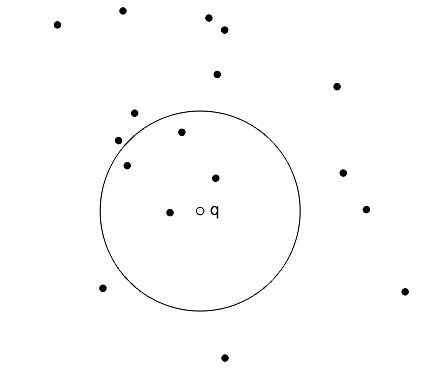
\includegraphics[width=.45\columnwidth]{gfx/range_query}} \quad
\subfloat[Nearest-Neighbour query] 
{\label{fig:nn_query}
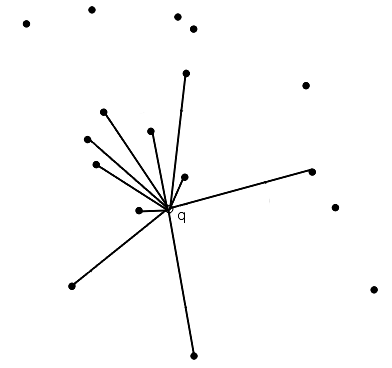
\includegraphics[width=.45\columnwidth]{gfx/nn_query}}
\caption[Range query and nearest-neighbours query in two dimensional Euclidean Space.]{Range query and nearest-neighbours query in two dimensional Euclidean Space.}
\end{figure}
%
\begin{mydef}
A nearest neighbour query is a function $NN:S \times \mathbb{Z}^+ \rightarrow S $ where $NN(q, k) = R \subseteq S$ such that $\forall x \in R, y \in S - R, d(q, x) < d(q,y) $ and $ |R| = k$.
\end{mydef}
%
%\begin{myexample}{Nearest Neighbour query example}
%\end{myexample}
% ********************** %
\section{Thesis outline}
% ********************** %
Having introduced the notion of similarity search in general terms, we now outline what follows in this thesis.  Part 1 introduces the mathematical preliminaries that underpin the work in subsequent parts.  It consists of a single chapter which covers aspects of distance, probability, and information theory that are pertinent.  This is followed in Part 2 with three chapters that deal with combining distance, probability and information theory. First, by introducing various methods of computing distance with information in chapter \ref{ch:information_distances}; Secondly, by narrowing the focus specifically to Structural Entropic Distance in chapter \ref{ch:multiway_structural_entropic_distance} and generalising it to the notion of multi-way distance; and thirdly, by exploring efficient means of evaluating Structural Entropic Distance.  After this, follows the final part, Part 3, which investigates the use of Structural Entropic Distance.  It consists three further chapters: Chapter \ref{ch:similarity_search}, investigates the performance of Structural Entropic Distance as a distance metric used with Similarity Search indexing techniques; chapter \ref{ch:information_retrieval}, explores a modification to Structural Entropic Distance to perform the traditional Information Retrieval task of searching for documents relevant to a set of keywords.  Finally, in chapter \ref{ch:clustering_classification_and_outlier_detection} we make use of the multi-way distance generalisation to perform classic data-mining techniques such as clustering, classification, and outlier detection.
%
\part{Mathematical Preliminaries}
%
%%************************************************
\chapter{Distance and Spaces}\label{ch:distance}
%************************************************


%
%************************************************
\chapter{Distance, Probability Spaces and Information Theory}\label{ch:distance_probability_spaces_and_information_theory}
%************************************************
%\begin{flushleft}{\slshape    
%    At the time, Nixon was normalizing relations with China.  
%    I figured that if he could normalize relations, then so could I} \\ \medskip
%    --- Edgar Codd
%\end{flushleft}
%
In this chapter we review the basics of information theory starting with a brief recap of probability, then introduce information, and finally derive entropy as defined by Shannon in his seminal work\cite{Shannon:1948} to serve as a foundation for later chapters.

\section{Distance}

% ********************* %
\subsection{Metric spaces}
% ********************* %
A metric space is simply a set of objects which have distances between them. Our own understanding of the physical world informs our intuition for the postulates of a metric -- there cannot be a negative distance; the distance between points is the same in both directions; if there is no distance between two objects they must be be at the same point (be the same object) -- likewise, there is no distance between two identical objects; and finally, there is no shorter distance between two objects by taking a detour through a third object.

These axioms are defined formally as follows:
%
\begin{mydef} 
A metric space $M$ is an ordered pair $(X,d)$ where $X$ is a set and $d: X \times X \rightarrow \mathbb{R}$ is a metric that defines the distance between elements in $X$. Furthermore, $d$ must satisfy the following properties:
 \begin{flalign*}
  &\quad \forall x,y \in X, 
  && d(x, y) \geq 0    \tag{positiveness}&\qquad &\\
  %
  &\quad\forall x,y \in X, 
  && d(x, y) = d(y, x) \tag{symmetry}&&\\
  %
  &\quad\forall x,y \in X, 
  && d(x, y) = 0  \Leftrightarrow  x = y \tag{reflexitivity}&&\\
  %
  &\quad\forall x,y,z \in X, 
  && d(x, z)  \leq d(x, y) + d(y, z) \tag{triangle inequality}&&
 \end{flalign*} 
\end{mydef}
% 
% ********************* %
\subsection{Vector spaces}
% ********************* %
Vector spaces are more specific than metric spaces, since they allow the elements of the space to be added or scaled to produce new elements.%\ToDo{Give more motivation for describing this}
\begin{mydef} 
A metric space $M = (V, d)$ is also a vector space if $V$ is closed under addition and multiplication operations.
%
Furthermore, the following axioms must hold for addition:
%
 \begin{flalign*}
  &\quad \forall \mathbf{x},\mathbf{y} \in V,  
  && \mathbf{x} + \mathbf{y} =  \mathbf{y} + \mathbf{x}  \tag{commutativity}&\qquad\qquad&\\
  %
  &\quad \forall \mathbf{x},\mathbf{y},\mathbf{z} \in V, 
  && (\mathbf{x}+\mathbf{y})+\mathbf{z}  = \mathbf{x}+(\mathbf{y}+\mathbf{z})  \tag{associativity}&&\\
  %
  &\quad \forall \mathbf{x} \in V, 
  && \mathbf{0} + \mathbf{x} = \mathbf{x}  \tag{identity}&&\\
  %
  &\quad \forall \mathbf{x} \in V,  
  &&\mathbf{x} + (-\mathbf{x}) = \mathbf{0} \tag{existence of additive inverse}&&
 \end{flalign*} 
%
The following axioms must hold for multiplication:
%
 \begin{flalign*}
  &\quad  \forall \mathbf{x} \in V, \forall a,b \in \mathbb{R}, 
  && a(b\mathbf{x}) = (ab)\mathbf{x}  \tag{associativity}&\qquad\qquad\qquad &\\
  %
  &\quad \forall \mathbf{x} \in V, 
  && 1\mathbf{x} = \mathbf{x}  \tag{identity}&&
 \end{flalign*} 
%
And the following laws of distributivity also:
%
 \begin{flalign*}
  &\quad \forall \mathbf{x} \in V, \forall a,b \in \mathbb{R},
  && (a+b)\mathbf{x} = a\mathbf{x} + b\mathbf{x}  \tag{scalar sums}&\qquad\qquad &\\
%  
  &\quad \forall \mathbf{x}, \mathbf{y} \in V,\forall a \in \mathbb{R},
  && a(\mathbf{x} +\mathbf{y}) = a\mathbf{x} + a\mathbf{y} \tag{vector sums}&&
 \end{flalign*} 
%
\end{mydef}
As a further refinement we now define a Normed Vector Space which adds the concept of magnitude to the elements of the space.%\ToDo{Give more motivation for describing this}
\begin{mydef} 
A normed vector space $N = (V, \|\cdot\|)$ where $V$ is a vector space and $\|\cdot\|: V \rightarrow \mathbb{R}$ a normalisation function.
%
Furthermore, the normalisation function must satisfy the following three properties:
\begin{flalign*}
  &\quad \forall \mathbf{x} \in V, 
  && \|\mathbf{x}\| > 0 \Leftrightarrow  \mathbf{x} \neq \mathbf{0} \tag{positivity}&\qquad\qquad\qquad &\\
%  
  &\quad \forall \mathbf{x} \in V,\forall a \in \mathbb{R}, 
  && \|a\mathbf{x}\| = |a|\|\mathbf{x}\| \tag{positive scalability}&&\\
%
  &\quad \forall \mathbf{x}, \mathbf{y} \in V,
  && \|\mathbf{x} + \mathbf{y} \| \leq \|\mathbf{x}\| + \|\mathbf{y}\| \tag{triangle inequality}&&
 \end{flalign*} 
\end{mydef}
As a final refinement to vector spaces, let us now add the concept of inner product.%\ToDo{Give more motivation for describing this}
%
\begin{mydef} 
A inner product space $I = (N, \langle\cdot, \cdot\rangle)$ where $N = (V, \|\cdot\|)$ is a normed vector space and $\langle \cdot, \cdot \rangle: V \times V \rightarrow \mathbb{R}$ an inner product function.
%
Furthermore, the inner product must satisfy the following three properties:
\begin{flalign*}
  &\quad \forall \mathbf{x}, \mathbf{y} \in V, 
  && \langle \mathbf{x}, \mathbf{y} \rangle 
  =\langle \mathbf{y}, \mathbf{x} \rangle  \tag{symmetry}&\qquad\qquad &\\
  %
  &\quad \forall \mathbf{x}, \mathbf{y} \in V,\forall a \in \mathbb{R}, 
  && \langle a\mathbf{x}, \mathbf{y} \rangle 
  = a\langle \mathbf{x}, \mathbf{y} \rangle \tag{scalar linearity}& &\\
  %
  &\quad \forall \mathbf{x}, \mathbf{y}, \mathbf{z} \in V, 
  && \langle \mathbf{x}+\mathbf{y}, \mathbf{z} \rangle 
  = \langle \mathbf{x}, \mathbf{z} \rangle + \langle \mathbf{y}, \mathbf{z} \rangle \tag{vector linearity}& &\\
  %  
  &\quad \forall \mathbf{x} \in V, 
  && \langle \mathbf{x}, \mathbf{x} \rangle 
  \geq  0 \tag{positive definiteness}& &
\end{flalign*}
\end{mydef}
\subsection{Distance Metrics}
%\ToDo{What is the motivation for describing all of these distance functions?}
Given these mathematical abstractions, we might ask what kind of distance functions exist that satisfy these axioms and what are they good for.  Let us start with a simple example, we would like to measure the similarity of two strings of characters.  This could be because we are building a spelling checker that might give suggestions of the most likely intended word.  It might also be required for a biologist working on DNA sequences that needs to find commonalities to identify some gene's function.
%\begin{myexample}{Edit Distance\ToDo{fix}}\label{dist:edit}
%\[
%d(x, y) = \begin{cases}
%            \max(i,j) &\mbox{if } \min(i,j) = 0 \\
%            \min \begin{cases} 
%                d(x-1, y) + 1\\
%                d(x, y-1) + 1\\
%                d(x-1, y-1) + [x \neq y]
%            \end{cases}&\mbox{otherwise} 
%\end{cases}
%\]
%\end{myexample}
%Example \ref{dist:edit} describes the edit distance or Levenshtein distance, this describes cost of a sequence of transformations that turns one string into another.
%%
%\begin{myexample}{Cosine Distance}
%\ToDo{Discuss}
%%
%\[
%  d_{\cos}(x,y) =  \cos^{-1}\left(\frac{x \cdot y}{|x| \cdot |y|}\right) \cdot \frac{2}{\pi} 
%\]
%\end{myexample}
%
%%
%\begin{myexample}{Minkowski Distances}
%\ToDo{Discuss}
%%
%Let $x, y \in \mathbb{R}^n$ 
%%
%\[ 
%  d_p(x, y) = \sqrt[p]{\sum_{i=1}^{n} | x_i - y_i |^p} 
%\]
%%
%\end{myexample}
%
%\begin{myexample}{Mahalanobis Distance}
%\ToDo{Discuss}
%%
%\[ 
%  d(x, y) = \sqrt{(x - y)M(x - y)^T} 
%\]
%\end{myexample}
%
%%
%\begin{myexample}{Jaccard Distance}
%\ToDo{Discuss}
%%
%\[ 
%  d(X,Y) = 1 - \frac{X \cap Y}{X \cup Y} 
%\]
%%
%\end{myexample}
%
%etc...
% ************************** %
\subsection{Space partitioning}
% ************************** %
As is typical with other types of storage system, partitioning the space allows for more efficient searching by excluding whole subsets from the search space, thus reducing effort required.  In contrast to other Spaces, (e.g. Vector Spaces), Metric Space and by implication the associated distance function contains very little information about the actual layout of the space.  It is, however, possible to use the properties of the metric, and in particular, triangle inequality to divide up the space in a principled way.  

\cite{Uhlmann:1991} introduced two techniques, \textit{Ball decomposition}, and \textit{Generalised Hyperplane decomposition} which have formed the basis of most index design to date; while \textit{Excluded Middle}, which extends \textit{Ball decomposition}, has been suggested by \cite{Yianilos:1999}.
%  
\subsubsection{Ball decomposition}
%
\begin{mydef}
Let $d_m$ be the median of $\{d(p, o_i), \forall o_i \in X\}$ for some pivot $p \in S \subseteq X$.  Partition $S$ into two subsets $S_1$ and $S_2$ such that $S_1 = \{o_j : d(p, o_j) \leq d_m\}$ and $S_2 = \{o_j : d(p, o_j) > d_m\}$
\end{mydef}
%
\begin{figure}
\centering
\subfloat[Ball Decomposition.] 
{\label{fig:ball_decomposition}
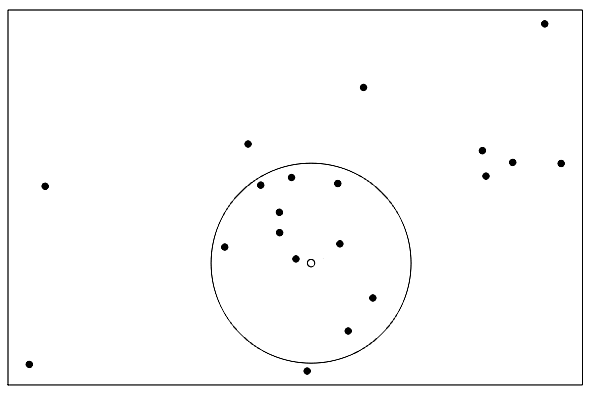
\includegraphics[width=.45\columnwidth]{gfx/ball_partition}} \quad
\subfloat[Generalised hyperplane Decomposition.] 
{\label{fig:hyperplane_decomposition}
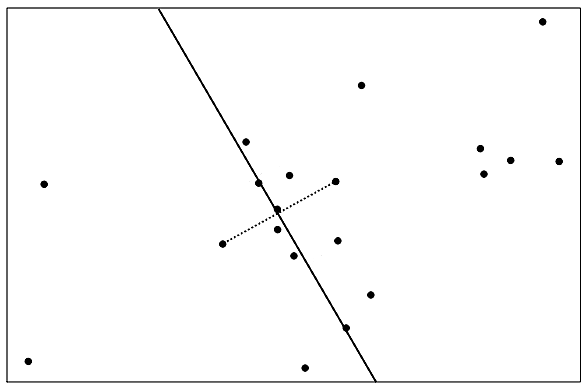
\includegraphics[width=.45\columnwidth]{gfx/hyperplane_partition}}
\caption[Ball Decomposition vs. Generalised hyperplane Decomposition]{Ball Decomposition -- the area inside the ball is one partition, the area outside is another.
Generalised hyperplane Decomposition -- those points nearest the first pivot form one partition, those nearest the other form another.}
\end{figure}
%
\subsubsection{Generalised hyperplane decomposition}
%
\begin{mydef}
Let $p_1$ and $p_2$ be two arbitary pivots selected from $S \subseteq X$.  Partition $S$ into two subsets $S_1$ and $S_2$ such that $S_1 = \{o_j : d(p_1, o_j) \leq d(p_2, o_j)\}$ and $S_2 = \{o_j : d(p_1, o_j) > d(p_2, o_j)\}$
\end{mydef}
% ********************** %
\subsection{Dimensionality}
% ********************** %
Bellman coined the term \textit{curse of dimensionality} referring to the exponential growth in the number of samples required to estimate a function with a given level of accuracy to its number of variables (or dimensions)\cite{Bellman:2003}.  This has a direct impact on similarity searching in that the number of points that must be visited to build the result of a query grows exponentially to the number of dimensions in the space.  In some cases, data may even be clustered together so tightly that the distance between the nearest neighbour and the farthest neighbour are the same, rendering any result meaningless.  In fact, it has been shown that these values converge as the number of dimensions increase%\cite{Indyk:1998}
%
\subsubsection{Measuring dimensionality}
Given the difficulty of indexing spaces with high dimensionality, a prudent approach would be to measure this. 
% [Here are the authors that have made a contribution, and what they have done]
%$d = \lim_{\epsilon \rightarrow 0} \frac{H_\epsilon(X)}{\log 1/\epsilon}$
%Intrinsic dimensionality
%
There is a great volume of work on the analysis of high-dimensional search spaces. Navarro gives a very elegant analysis of the history of this, along with some cogent insights into directions which could be usefully followed in the future, and bemoans the small volume of current research on the topic. 
%We follow his advice in that we attempt to find a general analysis rather than looking for reliance upon experiment or detailed analysis of particular data structures. Furthermore we also believe our analysis fulfils his longer-term goals of research in this domain which can underlie useful insight in the design of future techniques, rather than simply provide performance indicators.
%Other researchers also have advocated the analysis of performance based crucially upon the distribution of distances within the range of the metric over the objects of the space rather than on the data itself of the index structures, and we follow that lead.

%In \cite{}, a derivation for an exclusion probability e is given; this concept is technically equivalent to the probability pe we introduce in chapter \label{}, although we use a simplified version via the introduction of various assumptions. In spirit, this e is more similar to our IF , in that both are the probabilities of a pivoting operation failing to exclude some part of the data set from an exhaustive search.
%In the end, we deduce an outcome for the cost of a search in the order of (1 + IF ) ln n , rather than k + ne k , which is perhaps not inconsistent given that we use a much more restrictive indicative context.

%\subsection{Instrinsic Dimensionality}
%Our own work is more closely related to the description of Intrinsic Dimensionality as a performance predictor given in \cite{}. In particular it is applicable where the distance distribution strays from the ideal underlying Gaussian model, and where the fraction of data to be fetched is small.
%In common with \cite{}, the basis for measurement is only the set of distances produced by the metric with respect to the space, rather than the data itself, and our aim is to find a pragmatic measure of efficacy based only on the distribution of these distances. Both approaches allow for an automated assessment to be made only on presentation of a metric space with a random sampling mechanism.

The Intrinsic Dimensionality (IDIM) of a metric space is a measure defined over a distance histogram produced by the distance metric over the data. It is defined as
\[ 
\rho = \frac{\mu^2}{2\sigma^2}
\]
where $\mu$ is the expected distance and $\sigma^2$ is the variance of the range of the metric over the data collection. An IDIM of n corresponds roughly to the histogram of Euclidean distance over densely-populated n-dimensional Cartesian space. It is usually, but not always, the case that a higher value for IDIM leads to a worse performance of index structures for similarity search.

The authors give a lower bound for the cost of a pivoting operation as
\[ \left( \sqrt{\rho} - \frac{1}{\sqrt{2f}} \right)^2 \cdot \ln n\]
where $\rho$ is the IDIM, $f$ is the fraction of the data being returned, and $n$ is the size of the data. However this formula is valid only when $f > \frac{1}{2\rho}$, meaning that for large data sets, and therefore small values of $f$, it is of limited value.
The work uses an underlying assumption that the metric gives a Gaussian distribution of outcomes. 
%Figure 1 shows some distributions which are clearly not Gaussian; these are not artificially constructed, but show meaningful metrics in use over data sets within the SISAP collection [6].
More important, we believe, is that no metric distribution obeys a Gaussian distribution close to the origin as distances are by definition lower-bounded at zero, and we later show distributions very close to Gaussian where IDIM comparison is misleading as a predictor of performance.

In the discussion, the authors consider the same region of interest as here, the set of sampled distances which do not allow a median-centred pivot operation to successfully exclude any data from a search. 
%Our contributions over and above that are: (i) we note the fact that the distribution at the origin is crucially important in terms of selecting a value for the query threshold (t), and that the Gaussian model does not explain this; (ii) we note that the effect of t over the distribution is an effect of the standard deviation alone, and is unaffected by the value of the median, and (iii) by treating this region as a probability, by use of a probability density function rather than a histogram, we go on to calculate an actual indexing performance prediction based on a notional ball-pivot data structure.

%\subsubsection{Dimensionality reduction}
%Beyond simply measuring, some authors have approached the curse of dimensionality through a technique called dimensionality reduction. [Here are the authors that have made a contribution, and what they have done] 
%% *************** %
%\section{Summary}
%% *************** %
%In this chapter we have introduced the general concept of similarity search and justified its existence for types of data that do not lend themselves well to the existing methods of data storage.  We showed a useful mathematical abstraction called Metric Spaces, which allow us to reason about similarity in a way that produces efficient storage and retrieval.  Using the properties of Metric Spaces, we demonstrated the types of query that may be performed in such an abstraction, with emphasis placed on two in particular: range queries and nearest neighbour queries.  Next we quickly surveyed the principle metrics and data structures used in the storage and retrieval of data within the similarity search paradigm.  Finally we showed the limitations of using this abstraction, and in particular the curse of dimensionality with all of its negative implications.

% *************** %
\section{Probability \& Information Theory}
% *************** %
%\ToDo{Why are we looking at Probability?}
The frequentist view of probability is that there is a set of events that we assume occurs some number of times such that no two events can occur simultaneously. 
%
\begin{mydef}\label{prob}
let $E = \{ e_1, e_2, \ldots e_n \}$ be a sample space, some $F \subseteq E$ be an event space, and $P: E \rightarrow [0,1]$ a probability measure where $P$ satisfies the following axioms:
%
 \begin{align*}
  &P(F) \geq 0\\
  &P(E) = 1\\
  &P(\bigsqcup_{F \subseteq E} F) = \sum_{F \subseteq E} P(F)
 \end{align*}
%
\end{mydef} 
The probability must be positive, since a zero probability means it is certain not to happen you cannot be less certain of an event occurring than that.  The second axioms states that the probability that the next event occurring is from the set of all possible events is certain.  The third axiom states that the probability of an event occurring from the union of disjoint sets is the sum of probabilities from each of those disjoint sets. 
%
Furthermore the following derived properties also hold:
%
  \begin{align*}
  & P(\emptyset) = 0\\
  & P(F_1 \cup F_2) = P(F_1) + P(F_2) - P(F_1 \cap F_2)\\
  & P(E \setminus F) = 1 - P(F)
 \end{align*}
That is, the probability of an event occurring from the empty set is zero.  The probability of an event occurring from the union of two sets is the sum of  the probability of it coming from their respective sets minus the probability of the events that have been counted twice.  And the probability of an event occurring from outside a set is the probability of the sample space (which from the second axiom is 1) minus the probability of the event space.

A probability distribution assigns a probability to each subset.  
%Probabilities can be determined empirically as the number of times an event has occurred normalised by the total number of events.  
The proportion of times an event occurs relative to all events that have occurred is the probability of that event.

%\begin{myexample}
%Fair coin toss -- as is traditional when demonstrating probability.
%\end{myexample}
%
%\begin{myexample}
%Some other example
%\end{myexample}

% *************** %
\subsection{Information}
% *************** %
Suppose we have a probability function $P$, we can measure the information gained by observing an event based on the probability distribution of events.
%  
\begin{mydef}
Let $I: [0,1] \rightarrow \mathbb{R}$ be a monotonic function that measures the information gained by observing an event $e$ with probability $p = P(e)$, with the following axioms:
%
  \begin{align*}
  &\forall p, I(p) \geq 0\\
  & I(p) = 0 \Leftrightarrow p = 1\\
  & I(p_1 \cdot p_2) = I(p_1) + I(p_2)
  \end{align*} 
%
\end{mydef} 
%
The first axiom says that the information function must output a positive value;  it makes no sense to have lost information by witnessing an event.  The second says that there is no information to be gained by witnessing an event which we know is certain to occur.  The third says that the information gained after witnessing two events is the same as gaining the information from witnessing them separately.  A commonly used information function which obeys these axioms is $I(p) = -\log_b(p)$ for some base $b$.
%\begin{myexample}
%Some other example
%\end{myexample}
%\begin{myexample}
%Some other example
%\end{myexample} 
% *************** %
\subsection{Entropy}
% *************** %
%\ToDo{Why are we looking at Entropy?}
Given a stream of events whose probability is defined by the some function $P$ the average information gained per event is known as entropy.
%
\begin{mydef}
Let $S$ be some source emitting a stream of events from the set $E = \{e_1, e_2, \ldots, e_n\}$ with associated probabilities $P = \{p_1, p_2, \ldots, p_n\}$ respectively.

There are $N\cdot p_i$ occurrences of $e_i$ after $N$ observations, as $N$ approaches infinity.  So the total information gained is $I = \sum_{i = 1}^n (N \cdot p_i) \cdot I(p_i)$, and the average information per event is therefore:
\[ H(S) = \frac{I}{N} \]
Using $I(p_i) = -\log(p_i)$ gives,
\begin{align*}
H(S) &= \frac{1}{N} \cdot \sum_{i = 1}^n  (N \cdot p_i) \cdot -\log_b (p_i)\\
	 &= -\sum_{i = 1}^n  p_i \cdot \log_b (p_i)
\end{align*}  
\end{mydef}

%\begin{myexample}
%Some other example
%\end{myexample}
%\begin{myexample}
%Some other example
%\end{myexample}

\begin{mydef}
Let $S$ and $T$ be two sources emitting streams of events from the set $E = \{e_1, e_2, \ldots, e_n\}$.  Denote the probability of $S$ emitting $e_i$ and $T$ emitting $e_j$ as $p_{i,j}$.  Then the joint entropy of $S$ and $T$ is:
\[H(S, T) = -\sum_{i = 1}^n\sum_{j = 1}^n p_{i,j} \log_b (p_{i,j})\]
\end{mydef}

\subsection{Mutual Information}
\begin{mydef}
Let $S$ and $T$ be two sources emitting streams of events from the set $E = \{e_1, e_2, \ldots, e_n\}$. Then the mutual information between $S$ and $T$ is:
\[I(S,T) = H(S) + H(T) - H(S,T)\]
\end{mydef}

\subsection{Cross Entropy}
\begin{mydef}
Consider two sources, $S$ and $T$, emitting streams of events from the same set $E = \{e_1, e_2, \ldots, e_n\}$.  Let $S$ emit events with probability $P = \{p_1, p_2, \ldots, p_n\}$ and $T$ emit events with probability $Q = \{q_1, q_2, \ldots, q_n\}$.  If we model $S$ with $T$, $P$ is the true distribution and $Q$ is the model distribution. After $N$ observations, there are $N \cdot p_i$ occurrences of $e_i$, as $N$ approaches infinity, so the total information gained is $I = \sum_{i = 1}^n (N \cdot p_i) \cdot I(q_i)$, and the average information gained is:
\begin{align*}
H(S||T) 	&= \frac{I}{N}\\
	 	&= \frac{1}{N} \cdot \sum_{i = 1}^n  (N \cdot p_i) \cdot -\log_b (q_i)\\
	 	&= -\sum_{i = 1}^n  p_i \cdot \log_b (q_i)
\end{align*}  
\end{mydef}
This represents the average amount of surprise from observing an event when modelling a one distribution with another.
\subsection{Gibbs' inequality}
\begin{align*}
H(S||T) 	&\geq  H(S)\\
H(S||T) - H(S) &\geq 0\\
\end{align*}
The average amount of surprise when modelling one distribution with another is greater than if you had used the correct distribution.
\subsection{Relative Entropy}
This difference in entropies, $H(S||T) - H(S)$, is the relative entropy. Commonly known as K\"ullback-Liebler divegence; it is a measure of the divergence of information streams:
\begin{align*} 
KL(S||T)		&= H(S||T) - H(S)\\
			&= -\sum_{i = 1}^n  p_i \cdot \log_b (q_i) + \sum_{i = 1}^n  p_i \cdot \log_b (p_i)\\
			&= -\sum_{i = 1}^n  p_i \cdot (\log_b (q_i) - \log_b (p_i))\\
			&= -\sum_{i = 1}^n  p_i \cdot \log_b (\frac{q_i}{p_i})
\end{align*}
%The K\"ullback-Liebler divergence is derived directly from Shannon's original  definition of the entropy of a set of independent variables. Set in the context of a term-probability vector modelling a document $d$, the Shannon entropy is:
%%
%\[H_b(d) = - \sum_t \p(t|d) \log_b ( \p(t|d))\]

%In the context of the very sparse vectors used for the vector space model, it is worth explicitly noting that, for this purpose, the undefined term $0 \! \log(0)$ is normally taken as having a value of 0; this is reasonable as the term $\epsilon \log \epsilon \rightarrow 0$ as $\epsilon \rightarrow 0$.

%The meaning of the term $H_2(d)$ in our context is a theoretical lower bound for the mean number of bits%
%\footnote{From this point we will assume that all logs  are  base 2.}
% required to communicate each event in the stream generated by $\G^d$.

The information in event e for discrimination between distributions $P$ and $Q$, and the mean information for discrimination.
%For two generators $\G^v$ and $G^w$, then $KL(G^v,G^w)$ gives the extra  number of bits per event required to encode $G^w$ over $G^v$. This function is given by
%\[
%KL(v,w) = \sum_t  \p(t|v)  \log \! \left(\frac{\p(t|v)}{\p(t|w)}\right) 
%\]
As a general measure of difference, this function has a number of problems: it is asymmetric, unbounded, and undefined in the presence of zero values.

%The K\"ullback-Liebler divergence is derived directly from Shannon's original  definition of the entropy of a set of independent variables. For a  vector $v$ modelling a probability distribution, the Shannon entropy is:
%%
%\[H(v) = - \sum_{i} v_i \log ( v_i)\]

%In the context of the very sparse vectors used for the vector space model, it is worth explicitly noting that, for this purpose, the undefined term $0 \! \log(0)$ is normally taken as having a value of 0; this is reasonable as the term $\epsilon \log \epsilon \rightarrow 0$ as $\epsilon \rightarrow 0$.

%The meaning of the term $H(v)$ in our context is a theoretical lower bound for the mean number of bits%
%\footnote{if  base 2 logarithms are used}
% required to communicate each event in the stream of events corresponding to $v$.

%K\"ullback-Liebler is a measure of the divergence of information streams. For two probability vectors $v$ and $w$, then $KL(v,w)$ gives the extra  number of bits per event required to encode $w$ over the number required to encode  $v$. This function is given by
%\[
%KL(v,w) = \sum_i  v_i  \log \! \left(\frac{v_i}{w_i}\right) 
%\]
%As a general measure of vector difference, this function has a number of problems: it is asymmetric, unbounded, and undefined in the presence of zero values.

\subsection{Jensen-Shannon Divergence}
Lin \cite{Lin:1999}  further examined the $KL$ divergence and defined a modified function which shares the more desirable properties, and removes the undesirable ones.
\begin{mydef}
Consider two sources, $S$ and $T$, emitting streams of events from the same set $E = \{e_1, e_2, \ldots, e_n\}$.  Let $S$ emit events with probability $P = \{p_1, p_2, \ldots, p_n\}$ and $T$ emit events with probability $Q = \{q_1, q_2, \ldots, q_n\}$.  Consider a notional stream $U$ with probability distribution $R = \{r_1, r_2, \ldots, r_n\}$ for events in $E$ given by the function: 
\begin{equation*}
	P_R(e_i) = \frac{p_i + q_i}{2}
\end{equation*}

The Jensen-Shannon divergence is the average of the relative entropies, $KL(S||U)$ and $KL(T||U)$.
\begin{align*}
	JSD(S,T)		&= \frac{KL(S||U) + KL(T||U)}{2}\\
				&= \frac{-\sum_{i = 1}^n  p_i \cdot \log_b (\frac{r_i}{p_i}) -\sum_{i = 1}^n  q_i \cdot \log_b (\frac{r_i}{q_i})}{2}\\
				&= \frac{1}{2} \sum_{i = 1}^n	 p_i \cdot \log_b (\frac{p_i}{r_i}) + q_i \cdot \log_b (\frac{q_i}{r_i})
\end{align*}
\end{mydef}

%This function, generally known as Jensen-Shannon divergence, is given in its simplest form as
%\[
%JS(P,Q)  = KL(P,M) + KL(Q,M)
%\]
%where $M$ is the arithmetic  mean of $P$ and $Q$. 


%This function avoids the most problematic case, where the vectors $v$ and $w$ have a zero and a non-zero value respectively in the same dimension: as the vector $m$ is non-zero in that dimension, then  the $KL$ function is still well-defined%
%\footnote{division by zero is avoided but not $\log 0$; as both $\epsilon\log{\epsilon}$ and $\log \left(\frac{\epsilon}{\epsilon} \right)\cdot \epsilon \rightarrow 0$ as $\epsilon \rightarrow 0$ these terms are  taken as 0.}.

If base 2 logs are used, then the outcome is bounded in [0,1] with 0 meaning that the two distributions have equal probabilities for every event, and 2 meaning that for no event are both probabilities non-zero (see e.g. \cite{Lin:1999}). Despite being a simple derivation from K\"ullback-Liebler \cite{Lin:1999}, the Jensen-Shannon divergence is positive, symmetric, bounded and well-defined in all circumstances, and also has the identity property.

%There is a  form of Jensen-Shannon which is a proper distance metric. However, especially in the  context of sparse, high-dimensional vector spaces, even semantically close objects may have a significantly large threshold value. Intrinsic Dimensionality tends to be very high, even into the thousands; the combination makes the metric very poorly suited for metric search techniques.

Surprisingly recently, two authors \cite{endres:2003,OstVaj03} have independently established that the Jensen-Shannon divergence is the square of a proper metric. Since then, the metric has attracted some more interest in both statistics and information theory, and deeper analysis \cite{fuglede:paper} continues to show that the metric has some properties that, in short, should lend it to being, in many cases, the best possible semantic distance over any probabilistic generated form.
 
The fact that a form exists which is a proper metric immediately leads to the possibility of its use within metric indexing techniques. However any such excitement is short-lived in most cases; generative spaces are typically high-dimensional and sparse, and typical Intrinsic Dimensionality is very high -- possibly in the thousands -- excluding any possibility of successfully using metric indexing techniques.


%Kullback and Leibler describe the value $\log\frac{P_{x}(e)}{P_{y}(e)}$ as the information in event e for discrimination between distributions $x$ and $y$, and the mean information for discrimination -- nowadays known as the Kullback-Leibler divergence:
%\begin{align*}
%H(S) &= \frac{1}{N} \cdot \sum_{i = 1}^n  (N \cdot p_i) \cdot (\log_b (p_i) - \log_b(p_j))\\
%\end{align*} 
%
%
%\[
%KL(X,Y) = \sum_e P_{x}(e) \log\frac{P_{x}(e)}{P_{y}(e)}
%\]
%Jeffreys also used $\log\frac{P_{x}(e)}{P_{y}(e)}$ in %\cite{Jeffreys:1948} 
%but came up with a symmetrized version:
%\[
%J(X,Y) = \sum_e (P_{x}(e) - P_{y}(e)) \log\frac{P_{x}(e)}{P_{y}(e)}
%\]
%which turns out to have the value $KL(X,Y) + KL(Y,X)$.
%
%K\"ullback-Liebler divergence \cite{kullback_liebler} has been used to compare vector spaces in a number of different contexts. However it is of  limited use as a  general notion of dissimilarity: in particular, it is naturally asymmetric, unbounded, is not necessarily positive, and is undefined over any pair of distributions which contain zero probabilities. 

%Lin introduced the Jensen-Shannon divergence in \cite{Lin:1991} which is a symmetrized smoothed version of the Kullback-Leibler divergence:
%\begin{align}
%JSD(X,Y) &= \frac{KL(X,\frac{X+Y}{2}) + KL(Y,\frac{X+Y}{2})}{2}\notag\\
%&= \frac{\sum_e P_{x}(e) \log_2 \frac{P_{x}(e)}{P_{x \cup y}(e)} + \sum_e P_{y}(e) \log_2 \frac{P_{y}(e)}{P_{x \cup y}(e)}}{2}\notag\\
%&= \frac{1}{2}\sum_e P_{x}(e) \log_2 \frac{P_{x}(e)}{P_{x \cup y}(e)} + P_{y}(e) \log_2 \frac{P_{y}(e)}{P_{x \cup y}(e)}\label{eq:jsd}
%\end{align}


%Jensen-Shannon is the name commonly given to a divergence function first identified in \cite{Lin:1999}, in which some of the known deficiencies of the K\"ullback-Liebler divergence \cite{kullback_liebler} were investigated. We give a brief overview of the derivation.

%Lin \cite{Lin:1999}  further examined the $KL$ divergence  and defined a modified function which shares the more desirable properties, and removes the  undesirable ones. This function, generally known as Jensen-Shannon divergence, is given by
%\[
%JS(v,w)  = KL(v,m) + KL(w,m)
%\]
%where $m$ is the arithmetic  mean of $v$ and $w$. 

%This function avoids the most problematic case, where the vectors $v$ and $w$ have a zero and a non-zero value respectively in the same dimension: as the vector $m$ is non-zero in that dimension, then  the $KL$ function is still well-defined%
%\footnote{division by zero is avoided but not $\log 0$; as both $\epsilon\log{\epsilon}$ and $\log \left(\frac{\epsilon}{\epsilon} \right)\cdot \epsilon \rightarrow 0$ as $\epsilon \rightarrow 0$ these terms are  taken as 0.}.

%If base 2 logs are used and the result divided by two, then the outcome is bounded in [0,1] with 0 meaning that the two vectors have equal values in each dimension, and 1 meaning that for no dimension are both values non-zero \cite{Lin:1999}.
%% In this case, the function $D(v,w) = \sqrt{1 - JS(v,w)}$ is also a proper distance metric \cite{}.


% *************** %
\subsection{Kolmogorov Complexity}
% *************** %
Until now, we have discussed information in terms of random variables where entropy is average information.  Another approach instead  considers the actual information needed to specify strings of symbols.  The Kolmogorov complexity, $K(X)$, is the minimal length of any input which leads to the output $X$, for some fixed universal computer. The Kolmogorov complexity of the concatenation of two strings $X$ and $Y$, $K(XY)$, should be larger than $K(X)$ but cannot be larger than the sum $K(X)+K(Y)$
%\begin{quotation}\ToDo{paraphrase}
%In contrast to Shannon theory where the basic objects are random variables and entropies are average informations, algorithmic information theory deals with individual symbol strings and with the actual information needed to specify them. 
%To ``specify'' a sequence $X$ means here to give the necessary input to a universal computer $U$, such that $U$ prints $X$ on its output and stops. The analogon to entropy, called here usually the complexity $K(X)$ of $X$, is the minimal length of any input which leads to the output $X$, for fixed $U$. It depends on $U$, but it can be shown that this dependence is weak and can be neglected in the limit when $K(X)$ is large.
%
%Let us denote the concatenation of two strings $X$ and $Y$ as $XY$. Its complexity is $K(XY)$. It is intuitively clear that $K(XY)$ should be larger than $K(X)$ but cannot be larger than the sum $K(X)+K(Y)$. Even if $X$ and $Y$ are completely unrelated, so that one cannot learn anything about $Y$ by knowing $X$, $K(XY)$ is slightly smaller that $K(X) + K(Y)$. The reason is simply that the information needed to reconstruct $XY$ (which is measured by $K(XY)$) does not include the information about where $X$ ends and $Y$ starts (which is included of course in $K(X) + K(Y)$). The latter information increases logarithmically with the total length $N$ of the sequence $XY$. It is one of the sources for ubiquitous terms of order $\log(N)$ which become irrelevant in the limit $N \rightarrow \infty$, but make rigorous theorems in algorithmic information theory look unpleasant.
%\end{quotation}  
%
%\addtocontents{toc}{\protect\clearpage} % <--- just debug stuff, ignore
%
\cleardoublepage
%
\ctparttext{%
%
Information theory provides techniques for measuring the quantity of information contained within a given structure.  In this part, we introduce a new universal distance metric which is based upon the relative information content between two structures.  We show how this metric can be efficiently computed and how it compares to other algorithms in terms of relevance and accuracy.%
%
}
%
\part{Similarity with information theory}
%
%**********************************************************************************
\chapter{Information distances}\label{ch:information_distances}
%**********************************************************************************
%\begin{flushleft}{\slshape    
%    At the time, Nixon was normalizing relations with China.  
%    I figured that if he could normalize relations, then so could I} \\ \medskip
%    --- Edgar Codd
%\end{flushleft}
%
%SEE:\cite{Wong:1985, Lin:1991, Menendez:1997, Kullback:1951}\\
%--------------------------------------------------------------------------------------------------%
In this chapter, we explore the measurement of structural similarity in structured data.  Since increasingly more information is stored in semi-structured data formats such as XML, it makes sense not only to measure the similarity of the textual content (as in traditional information retrieval) but of its structural meta-data too. This can be very useful when, for example, extracting document types, integrating heterogeneous data sources, merging data while cleaning it, or query by example.
\section{Compression based distances}
%%%%%%%%%%%%%%%%%%%%%%%%
%\ToDo{Paraphrase All of this!}
%%%%%%%%%%%%%%%%%%%%%%%%
If Kolmogorov complexity measures the absolute information content of an object, a similarly defined measurement of information distance between two objects is the minimal information required to generate either from the other.  This measure is universal, covering all other alternative informational distances as special cases, and machine-independent.  This universality, however, prevents its computability.\cite{}

The information distance between $x$ and $y$ is the length of the shortest program to transform $x$ into $y$ and $y$ into $x$, and, up to a logarithmic additive term, is equal to the maximum of the conditional Kolmogorov complexities, which is the length of the shortest program with input $y$ that outputs $x$\cite{}.  Because it is asymmetric, the conditional complexity $K(y|x)$ alone is an unsuitable information distance, thus the algorithmic informational distance between x and y is the sum of the relative complexities, $K(y|x)+ K(x|y)$. This overestimates the information required to translate between $x$ and $y$ in case there is some redundancy between the information required to get from $x$ to $y$ and the information required to get from $y$ to $x$.

\subsection{Normalised Compression Distance}
Bennet et al. introduced an information metric between data objects in \cite{}, in which they defined information distance (ID) 
\begin{equation}
	ID(x, y) = \max \{K(x|y), K(y|x)\}
\end{equation}
and its normalized version (NID):
\begin{equation}
    NID(x, y) = \frac{\max \{K(x | y), K(y | x)\}}{\max \{K(x), K(y)\}}
\end{equation}
They also showed it to have, despite minor infringements, metric properties.  

Although, as we have discussed, Kolmogorov complexity is not computable, it can be viewed as the length of the best possible compression of $x$. The best compression, however, is also not computable, but it is approximated using standard compression algorithms. In \cite{}, Cilibrasi and Vitanyi defined a normalized compression distance (NCD), derived from NID, replacing the denominator $K(x)$ with $C(x)$, which is the length of the compressed x, and the numerator first to 
\begin{equation}
\max\{K(x, y) - K(x), K(x, y) - K(y)\}
\end{equation}
exploiting the additive property of Kolmogorov complexity \cite{}, then -- as it is easier to handle concatenation with compression -- to \begin{equation}
\min\{C(xy), C(yx)\} - \min\{C(x), C(y)\}
\end{equation} The symmetry of many compression algorithms allows a further simplification to 
\begin{equation}
C(xy) - \min\{C(x), C(y)\}
\end{equation}
arriving at the definition of NCD found in \cite{}
\begin{equation}
    NCD(x, y) = \frac{C(xy) - \min \{C(x), C(y)\}}{\max \{C(x), C(y)\}}
\end{equation}

\subsection{Crossparsing Distance}
Ziv and Merhav\cite{} showed that crossparsing two sources can be used to approximate the relative entropy (or KL-divergence) between them, in the same way that the Lempel-Ziv\cite{} showed self-parsing (compression) approximates the entropy of a single source.  In \cite{}, Helmer defined crossparsing distance (CPD) using a generalized definition of crossparsing to allow sequences of differing length. 

%\begin{myexample}{Crossparsing}
%Crossparsing a string $x$ with respect to string $y$ is defined as follows: First, find the longest prefix of $x$ that appears as a string in $y$, %i.e., find the largest integer $k$ such that $x_1, x_2, \ldots, x_k = y_i, y_{i+1}, \ldots, y_{i+k-1}$ for some $i$.  After determining the first %value for $k$, we find the longest prefix of $x$ starting with $x_{k+1}$ with respect to $y$. We continue doing so until we have parsed the whole %word $x$. The crossparsing of $x$ with respect to $y$ is the set of all resulting phrases of $x$ and is denoted with $s(x|y)$.  For example, the %crossparsing of word $x = abbbbcaabba$ with respect to word $y = baababaabba$ is the set of phrases $s(x|y) = \{abb, bb, c, aabba\}$. 
%\end{myexample}

They defined CPD by normalising and symmetrising as follows:  First, using the codebook $s(x|y)$ -- which is the multiset of phrases of $x$ resulting from the crossparsing of $x$ with respect to $y$ -- they normalize to $\frac{|s(x|y) \setminus {y}|}{|x|}$, by observing that there is at least one phrase if $x$ is found as a substring of $y$ and at most $|x|$ phrases, thus $1 \leq |s(x|y)| \leq |x|$. This gives the value 0 if $x = y$, and a maximum value of 1. Note that $s(x|y) \setminus {y}$ removes a single copy of $y$ from the multiset $s(x|y)$, even if multiple copies exist. Secondly, a symmetric distance arises by taking the mean of normalised crossparsing both ways:
\begin{equation}
CPD(x, y) = \frac{1}{2}\left(\frac{|s(x|y) \setminus {y}|}{|x|} + \frac{|s(y|x) \setminus {x}|}{|y|}\right)
\end{equation}

Helmer found CPD performed better than the NCD at clustering and classification tasks, showing the limitation of compression distance: there is only a certain window when the difference between two data objects is measured. The Gzip algorithm first builds a dictionary for $x$; the difference between $x$ and $y$ is only measured when $y$ is parsed, since at that point $y$ is encoded using a code created for $x$. As the parsing of $y$ continues, more of the encoding will rely on the parts of $y$ that has already been scanned and less from the dictionary for $x$. Puglisi et al. \cite{} interpret this as a process in which the compression algorithm learns how to encode $y$ and unlearns how to do so for $x$. CPD, however, does not display this effect, since $x$ is used to encode $y$ and vice versa, thus, avoiding the consideration of self-similarity when comparing objects.

The trouble with both CPD and NCD is that neither is a true metric.  CPD does not satisfy triangle inequality, and while NCD satisfies triangle inequality up to an additive constant, this is not very pragmatic for similarity search.
%--------------------------------------------------------------------------------------------------%
\section{Statistical distances}
%
Where Kolmogorov Complexity is the absolute information content of an object, entropy is its expected information content and a limit on its best possible compression\cite{}.  The compression distances above all rely on a string representation of the objects to compress and derive an approximate value for Kolmogorov Complexity; in the following, we consider the statistical properties of an object to derive its entropy directly. We calculate a form of structural complexity, which we use as the basis for a distance function.  Avoiding Kolmogorov complexity in this way allows a computable function that does not rely on approximation.

%The similarity of structures is quantified in terms of a relationship between their individual complexities and the complexity of a theoretical merge. 
\subsection{Structural entropic distance (SED)}
%
Recall that the Kolmogorov Complexity of a string is the size of the smallest program that generates that string.  We require structural complexity  to behave much the same way for structured objects: The joint complexity should equal the individual complexities when both structures are identical, and should equal the sum of the individual complexities when there is no common structure.  

Consider a structured object as a conceptual generator of a stream that represents all possible navigation operations.  Suppose an infinite process of random traversals gives the probability of a traversal; the collection of all traversals with associated probabilities is called an ensemble.  Let $X$ be the source emitting the stream of navigation events $E = \{ e_1, e_2, \ldots, e_n \}$ with associated probabilities $P = \{ p_1, p_2, \ldots, p_n\}$. Assuming each traversal is independent the entropy of the stream is:  
\begin{equation}
	H_b(X) = -\sum_i p_i \log_b p_i
\end{equation}
which is the average information of the events in the stream $E$.  To eliminate the dependence on the logarithmic base we define the structural complexity
\begin{equation}
	C(X) = b^{H_b(X)}
\end{equation} 

In Algorithmic information theory, joint complexity is the complexity of the concatenation of two strings\cite{}; with structured data, however, this approach would be undesirable, since concatenation does not represent a merge.  Instead we merge  the streams event by event, taking half from each.  Formally, let $X$ and $Y$ be the sources emitting the streams $E$ and $F$; let $Z$ be the notional source emitting the merged stream $G = \{g_1, g_2, \ldots, g_n\}$ where $E \subseteq G$ and $F \subseteq G$, then  
\begin{equation}
	P_Z(g_i) = \frac{P_X(g_i) + P_Y(g_i)}{2}
\end{equation}

We define structural entropic distance, notionally, as the ratio of the joint complexity to the geometric mean of individual complexities, normalised into the range $[0,1]$, which can now be defined concretely using structural complexity: 
\begin{equation}
SED(X,Y) = \frac{C(Z)}{\sqrt{C(X) \cdot C(Y)}} - 1
\end{equation}
This distance is guided by the requirements of having a distance based on the amount of overlap of structural similarity. 
\nociteown{Moss:2013,Connor:2013a,Connor:2013b,Connor:2012,Connor:2011,Connor:2011a}
\nociteothers{Moss:2013, Connor:2013a,Connor:2013b,Connor:2012,Connor:2011,Connor:2011a}
\subsection{Relationship to Jensen-Shannon divergence}
The above distance function turns out to have a great deal of commonality with the Jensen-Shannon divergence (JSD), as shown by Theorem \ref{proof:JS}, and is a semantically compelling metric; for any data type that can be characterised by an ensemble of event-probability pairs, the Jensen-Shannon similarity gives an estimate of the probability of that data's having been output by the same probabilistic generator.
\begin{mytheorem}{$SED(x,y) = b^{JSD(x,y)} - 1$}
\begin{proof}\label{proof:JS}\footnotesize
\begin{align}
SED(X,Y) &= \frac{C(Z)}{\sqrt{C(X) \cdot C(Y)}} - 1\\
%
&= \frac{b^{H_b(Z)}}{\sqrt{\strut b^{H_b(X)} \cdot b^{H_b(Y)}}} - 1\\
%
&= \frac{b^{H_b(X)}}{\strut b^{\frac{1}{2}(H_b(X) + H_b(Y))}} - 1\\
%
&= b^{H_b(Z) -\frac{1}{2}(H_b(X) + H_b(Y))} - 1
\end{align}
Consider now only the exponent:
\begin{equation}
H_b(Z) -\frac{1}{2}(H_b(X) + H_b(Y))
\end{equation}
Substituting in the definition of entropy:
\begin{equation}
-\frac{1}{2}\sum_e 2 \cdot P_{Z}(e) \log_b P_{Z}(e) - P_{X}(e) \log_b P_{X}(e) - P_{Y}(e) \log_b P_{Y}(e)
\end{equation}
and rewriting in the positive:
\begin{equation}
\frac{1}{2}\sum_e -2 \cdot P_{Z}(e) \log_b P_{Z}(e) + P_{X}(e) \log_b P_{X}(e) + P_{Y}(e) \log_b P_{Y}(e)
\end{equation}
and substituting in the definition of $P_{Z}(e)$
\begin{equation}
\frac{1}{2}\sum_e -(P_{X}(e) + P_{Y}(e)) \log_b P_{Z}(e) + P_{X}(e) \log_b P_{X}(e) + P_{Y}(e) \log_b P_{Y}(e)
\end{equation}
then simplifying
\begin{equation}
\frac{1}{2}\sum_e P_{X}(e)\cdot ( \log_b P_{X}(e) - \log_b P_{Z}(e)) + P_{Y}(e) \cdot ( \log_b P_{Y}(e) - \log_b P_{Z}(e))
\end{equation}
and combining logs gives:
\begin{equation}
\frac{1}{2}\sum_e P_{X}(e) \log_b \frac{P_{X}(e)}{P_{Z}(e)} + P_{Y}(e) \log_b \frac{P_{Y}(e)}{P_{Z}(e)}
\end{equation}
which as shown in equation \ref{eq:jsd} is the Jensen-Shannon divergence, thus,
\begin{equation}
SED(X,Y) = b^{JSD(X,Y)} - 1
\end{equation}

\end{proof}
\end{mytheorem}

In this context, the JSD is considered as an assessment of the difference of two independent probability distributions: that is, where a randomly sampled event has a number of different possible outcomes, each with its own assigned probability.

This probabilistic divergence model can be applied to many other data sets, essentially any set of data whose semantics can be usefully captured in a vector space model. For example, in Information Retrieval, the unigram generative model (see e.g. \cite{manning:book,rijsbergen:1979}) has long been successfully used as a basis of similarity estimation among documents. In this model, a document is essentially reduced to a probabilistic generator, generating the terms within the document with probabilities in ratio to the number of appearances of each. Any such probabilistic metric can then be applied over these probability distributions to give a measurement of document similarity.  We look at this further in chapter \ref{ch:ir}.  Many other contexts, for example the extraction of image features, can also be viewed as such a probabilistic generative process.
%--------------------------------------------------------------------------------------------------%
\section{Structured data}
Both compression-based and statistical distances require, for structural comparison, a representation of the structured object that excludes the content, leaving only the structural information.  With compression based distances only a string representation is required, so a traversal that outputs the structural data is sufficient.  Statistical distances, however, require a distribution of events to be constructed upon which a probabilistic model is built; this requires a series of random traversals, meanwhile keeping track of the frequency of structural events.

\subsection{String representations}
In his comparison of NCD and CPD, Helmer\cite{} used four different methods to extract structural information from XML documents
\begin{description}
\item[Tags] Strip XML documents of all content (e.g. text nodes and attribute values) and extract all other nodes in document order by outputting their tag names (both opening and closing) and possible attribute names.
\item[Pairwise] Remove all content from the XML document and keep the remaining structural nodes. For each node, however, prepend the name of the parent node to its name. Again the document order is maintained but no closing tags are output.
\item[Full Path] After removing the content, prepend node names to the full path from the root node to the current node.
\item[Family Order] Family Order traversal represents a compromise between breadth-first and depth-first traversal. All the children of a node are output en bloc. However, before doing so, all their descendants have to be processed. 
\end{description}

%One could argue that describing the structural information of an XML document in a breadth-first manner is as appropriate as traversing it in document order. However, breadth-first traversal is problematic due to its memory consumption: given an XML document of height h, breadth-first traversal may need space that is exponential in h, whereas depth-first traversal uses up space that is linear in h.  In this way we still manage to keep the sibling information intact without having to store whole levels of the tree during the traversal.
\subsection{Statistical representation}
Extracting structural information for Statistical distances require a little more treatment; using the tree as a conceptual generator of events, an event stream is output by a random walk of the tree.  These events collectively form an ensemble of event-probability pairs from which the entropy is calculated.
\begin{figure}\footnotesize
\trimbox{0mm 0mm 0mm -10mm}{\begin{tikzpicture}[level/.style={sibling distance=60mm/#1}, edge from parent/.style={draw,-latex}]
\node [draw] (z){People}
  child {node [draw] (a) {Person}
    child {node [draw] (b) {Name}
        child {node [draw] (d) {Firstname}}
        child {node [draw] (e) {Surname}}
    }
    child {node [draw] (g) {Age}
    }
  }
  child {node [draw] (j) {Person}
    child {node [draw] (l) {Name}
      child {node [draw] (o) {Firstname}}
      child {node [draw] (p) {Surname}}
    }
    child {node [draw] (k) {Age}}
};
\end{tikzpicture}
}\\
\trimbox{0mm 0mm 0mm -10mm}{\begin{tikzpicture}[edge from parent/.style={draw,-latex}]
\tikzstyle{level 1}=[sibling distance=70mm] 
\tikzstyle{level 2}=[sibling distance=22mm] 
\node [draw] (z){People}
  child {node [draw] (a) {Person}
    child {node [draw] (c) {Name}}
    child {node [draw] (d) {D.O.B}}
    child {node [draw] (e) {Organisation}}
  }
  child {node [draw] (b) {Person}
    child {node [draw] (f) {Name}}
    child {node [draw] (g) {D.O.B}}
    child {node [draw] (h) {Organisation}}
  };

\end{tikzpicture}
}\caption{Trees used to generate an ensemble of events}
\label{ex:tree}
\end{figure}

\begin{table}\footnotesize
\centering
\begin{tabular*}{\textwidth}{l @{\extracolsep{\fill}}lrrr}
\toprule
event $e$		&$P_X(e)$\		&$P_Y(e)$		&$P_{Z}(e)$\\
\midrule
/People & $\frac{1}{33}$ & $\frac{1}{23}$ & $\frac{56}{759}$\\
/People/Person & $\frac{2}{33}$ & $\frac{2}{23}$ & $\frac{112}{759}$\\	
/People/Person/Name & $\frac{2}{33}$ & $\frac{2}{23}$ & $\frac{112}{759}$\\	
/People/Person/Age & $\frac{2}{33}$ & 0 & $\frac{1}{33}$\\
/People/Person/D.O.B & 0 & $\frac{2}{23}$ & $\frac{1}{23}$\\	
/People/Person/Organisation & 0 & $\frac{2}{23}$ & $\frac{1}{23}$\\
/People/Person/Name/Firstname & $\frac{2}{33}$ & 0 & $\frac{1}{33}$\\
/People/Person/Name/Surname & $\frac{2}{33}$ & 0 & $\frac{1}{33}$\\
/Person & $\frac{2}{33}$ & $\frac{2}{23}$ & $\frac{112}{759}$\\
/Person/Name & $\frac{2}{33}$ & $\frac{2}{23}$ & $\frac{112}{759}$\\
/Person/Age & $\frac{2}{33}$ & 0 & $\frac{1}{33}$\\
/Person/D.O.B & 0 & $\frac{2}{23}$ & $\frac{1}{23}$\\
/Person/Organisation & 0 & $\frac{2}{23}$ & $\frac{1}{23}$\\
/Person/Name/Firstname & $\frac{2}{33}$ & 0 & $\frac{1}{33}$\\
/Person/Name/Surname & $\frac{2}{33}$ & 0 & $\frac{1}{33}$\\
/Name & $\frac{2}{33}$ & $\frac{2}{23}$ & $\frac{112}{759}$\\
/Name/Firstname & $\frac{2}{33}$ & 0 & $\frac{1}{33}$\\	
/Name/Surname & $\frac{2}{33}$ & 0 & $\frac{1}{33}$\\
/Age & $\frac{2}{33}$ & 0 & $\frac{1}{33}$\\	
/Firstname & $\frac{2}{33}$ & 0 & $\frac{1}{33}$\\	
/Surname & $\frac{2}{33}$ & 0 & $\frac{1}{33}$\\	
/D.O.B & 0 & $\frac{2}{23}$ & $\frac{1}{23}$\\	
/Organisation & 0 & $\frac{2}{23}$ & $\frac{1}{23}$\\	
\bottomrule
\end{tabular*}
\caption{all of the events generated by random walks and their probabilities}
\label{event_table}
\end{table}

Consider the two trees in example \ref{ex:tree}, a stream of events is generated by a \textit{random walk} markov process over the tree structure.  A start node is selected at random, then at each step either an edge is traversed or the process is exited. Once the process is exited the resultant path forms an event in the probability space. An equivalence relation is formed on paths that contain a sequence of nodes with identical labels, that is, two different paths may be considered an instance of the same event if their sequence of node labels are identical.  We can then calculate the probabilities of the events by simply enumerating all possible paths in the tree and counting the occurrences of each event.  Table \ref{event_table} shows the probabilities of each event in both trees, along with the probabilities of the merged stream.

\subsection{Mapping to a vector space}\label{vector_space}
Many important similarity applications make use of the vector space model, where data objects can be represented as points in a space (for more information consult chapter \ref{ch:distance}).  The compression based distances do not lend themselves to this kind of treatment, not least because they do not satisfy Triangle Inequality.  The statistical distances do, however.

Using this mapping, tree structured data can easily be adapted to existing similarity applications.  We can, furthermore, now treat trees simply as vectors in a vector space and benefit from the abstraction knowing that any mathematical treatment applies to the whole domain, and indeed any other.  We now show the mapping from a frequency table of events to a vector space, and the calculation of JSD for vectors in $\mathrm{R}^n$.

Consider an inner product space over $\mathrm{R}^n$, where each dimension $x_i$ corresponds to a count of event $e_i$.  We use the norm: 
\begin{align}
    \|\mathbf{x}\|_1 &= \sum_{i=1}^{n} |x_i|
\intertext{to produce the unit vector:}
    \hat{\mathbf{x}} &= \frac{\mathbf{x}}{\|\mathbf{x}\|_1}
\intertext{where each $\hat{x}_i$ corresponds to the probability of observing event $e_i$.  Now, let the information vector of $\mathbf{x}$ be:}
    \mathbf{i}_x &= -\log_b(\hat{\mathbf{x}})
\intertext{where each $i_j$ is the amount of information gained by observing event $e_j$.  We can use the inner product:}
\langle \mathbf{x}, \mathbf{y}\rangle &= \sum_{i=1}^n x_i y_i
\intertext{to calculate the entropy as the inner product of the unit vector $\hat{\mathbf{x}}$ and the information vector $\mathbf{i}_x$:}
    H_b(\mathbf{x}) &= \langle \hat{\mathbf{x}} , \mathbf{i}_x\rangle
\intertext{which is the total information in the vector $\mathbf{x}$.	  And finally calculate the Jensen-Shannon divergence as,} 
	JSD(\mathbf{x}, \mathbf{y}) &= H_b(\mathbf{z}) - \frac{1}{2}(H_b(\mathbf{x}) + H_b(\mathbf{y}))
\end{align}
where $\mathbf{z} = \frac{\hat{\mathbf{x}} + \hat{\mathbf{y}}}{2}$ is the centroid of the unit vectors.
\begin{figure}
  \centering
  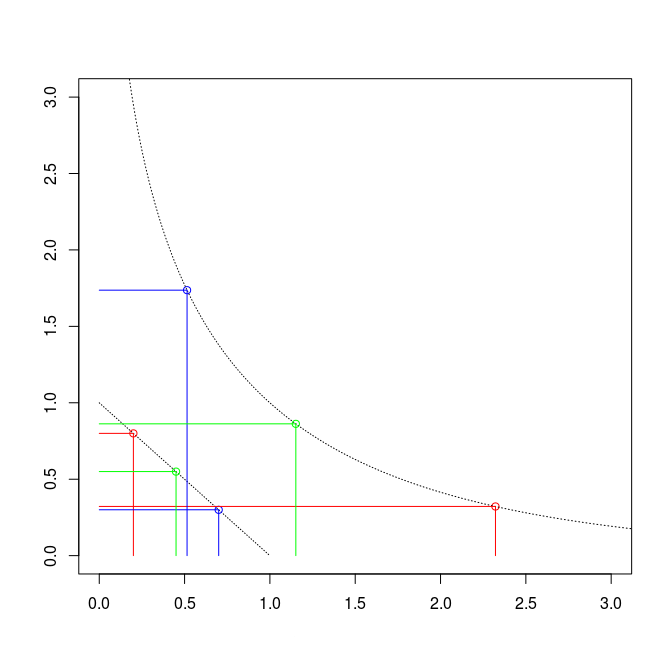
\includegraphics[width=4in]{gfx/sed_vector}
  \caption[Calculating distance]
   {In two dimensions -- The unit vectors $\hat{\mathbf{x}}$ (red), $\hat{\mathbf{y}}$ (blue), and $\hat{\mathbf{z}} = \frac{\hat{\mathbf{x}} + \hat{\mathbf{y}}}{2}$ (green) are on the $L^1$ norm; and the information vectors (using base 2), $\mathbf{i}_x$, $\mathbf{i}_y$, $\mathbf{i}_z$ are on the curved line.  The entropy is the dot product of the unit vector and information vector.  As the unit vector moves to the extremes in one direction the }
   \label{fig:entropic_space}
\end{figure}

Plotting some of these vectors in two-dimensional spaces gives us some intuition for how this function behaves.  As figure \ref{fig:entropic_space} demonstrates, the highest entropies occur when the normalised points lie at the extreme ends of the norm; by implication distances are far larger at the extremes than its Euclidean representation might suggest.  When a point has one dimension that is very low, it pushes that point much further away from other points that do not.  And this is, in fact, desirable behaviour for many similarity applications, such as clustering.  
%--------------------------------------------------------------------------------------------------%

%--------------------------------------------------------------------------------------------------%
\section{Conclusion}
This chapter has shown that existing information theoretic measures of structural distance based upon compression may not be suitable for similarity search.  We have produced an alternative, SED, that uses entropy at its core, which in turn has many commonalities with Jensen-Shannon Divergence.  

The transformation of JSD for use with metric searching prohibitively increases its dimensionality.  We have shown that SED, however, which can be used in its raw form for tree structured data, allows for much greater pruning opportunities with a metric index.  Furthermore, through algebraic manipulation, it can be calculated efficiently; by using an inverted index data structure, and, for range queries, early termination, this saving is as much as two orders of magnitude.

%

%************************************************
\chapter{Multiway Structural Entropic Distance}\label{ch:multiway_structural_entropic_distance}
%************************************************
%\begin{flushleft}{\slshape    
%    At the time, Nixon was normalizing relations with China.  
%    I figured that if he could normalize relations, then so could I} \\ \medskip
%    --- Edgar Codd
%\end{flushleft}
%
Much of the research on similarity search focuses on the similarity (or distance) between two objects.  For many situations, however, ascertaining the mutual similarity of a set of objects would be useful. Applications could be, for example, similarity joins, clustering, cluster analysis, and potentially many more that are dependent upon these techniques.

The calculation of density, or multi-way divergence as the analogue to distance, has been rarely used and is typically calculated through some compound function over the set of pair-wise distances within the set of objects: for example, the mean inter-set distance or the mean distance from each object to a centroid.  
%If the divergence function is used frequently, a large number of calls may be required of the, typically expensive, distance metric, making this type of operation prohibitively expensive.

In this chapter, we derive a function to calculate the divergence of a set of objects that is based on the structural entropic distance discussed in chapter \ref{ch:sim_structured_data}.  This new metric, which is grounded in information theory, avoids the problem of repeated calls to the distance metric through a direct, calculable notion of multi-way divergence without relying on approximation.  It reuses the notion of complexity offered in the definition of the original distance metric and reverts to this definition when the size of the set is two.  It is bounded, giving a maximum value when there is no commonality, allowing absolute comparisons to be made.  And finally, it is only a little more expensive than a single distance to evaluate.

We show that multi-way divergence offers a cheaper alternative to compound functions whilst giving similar, or better, semantic properties.  We believe it could be applied usefully to construct new metric indices or to execute more complex queries, such as similarity joins, efficiently. 
\section{Multiway distances}
The notion of a multi-way distance metric is not new,  motivation coming from geometry and topology.  Recently a few papers have  analysed the generalisation to multi-way for any existing metric\cite{Warrens2009, Warrens2010, Deza2000797}.  They consider whether various axioms are observed in these generalisations. For example, a metric space with a simple dyadic metric has the following axioms:
%
\begin{equation*}
\begin{aligned}
    d(x, y) &= 0 \Leftrightarrow x = y \\
    d(x, y) &= d(y, x) \\
    d(x, y) &\leq d(x, z) + d(y, z)
\end{aligned}
\end{equation*}
%
The first of these, is simply generalised to $D(x_1, \ldots, x_n) = 0$ if and only if all $x_i$ are equal; the second to $D(x_{\pi(1)}, \ldots, x_{\pi(n)}) = D(x_1, \ldots, x_n)$ for every permutation $\pi$ of $\{1, 2, \ldots, n\}$; while the third, triangle inequality, has been generalised in numerous ways\cite{Warrens2010}, such as polyhedron inequality:
%
\begin{equation*}
    (n - 1) \cdot D(x_1, \ldots, x_n) \leq \sum_{i = 1}^n D(x_1, \ldots, x_{i-1}, x_{i + 1},\ldots, x_{n+1})
\end{equation*}
%

These generalised axioms are interesting in their own right, and the first two  are desirable properties of a multi-way divergence function, but it is not clear if polyhedron inequality aids similarity search at this stage.
\subsection{Compound metrics} 
Deza and Rosenberg introduced the multi-way extension of the star distance in \cite{Deza2000797}, while perimeter distance\cite{Warrens2010} gives a geometrical ``average distance''.  Both of these, however, are compound functions and do not fundamentally look at generalising any specific metric.


\subsection{Multiway structural entropic distance (MSED)}

Let $X_1, \ldots X_n$ be the sources emitting the streams $E_1, \ldots E_n$; let $Y$ be the notional source emitting the merged stream $F = \{f_1, f_2, \ldots, f_m\}$ where $\forall E_i,  E_i \subseteq F$, then  
\begin{equation}
	P_Y(f_i) = \frac{\sum_{j=1}^n P_{X_j}(f_i)}{n}
\end{equation}
Recall from chapter \ref{ch:sim_structured_data} that the complexity of a source $X_i$ is given by the logarithmic base $b$ raised to the power of the entropy $H_b(X_i) = -\sum_{e \in E_i} P_{X_i}(e) \log_b P_{X_i}(e)$ of that source, $C(X_i) = b^{H_b(X_i)}$.  

Using the same principle as before of applying the ratio of the complexity of the merged stream to the geometric mean of individual complexities, we arrive at the ratio 
\begin{equation}
\frac{C(Y)}{\sqrt[n]{\prod_{i=1}^n C(X_i)}}
\end{equation}
which gives a value in the range $[1, n]$; we scale this to $[0,1]$ to give the multiway structural entropic distance:

\begin{equation}
MSED(X_1, \ldots X_n) = \frac{1}{n - 1} \cdot \left(\frac{C(Y)}{\sqrt[n]{\prod_{i=1}^n C(X_i)}} - 1\right)
\end{equation}

As it should, the joint complexity equals the individual complexities when all structures are identical, and equals the sum of the individual
complexities when there is no common structure.

Using the same mapping to vector spaces as before, this generalised function remains a ratio of the complexity of a centroid to the geometric mean of its neighbours' complexities, and has the following properties:  
\begin{itemize}
\item If all vectors are identical it gives 0
\item If all vectors are different it gives 1
\item All other inputs give a value between these bounds
\end{itemize}

Consider now the metric space axioms described at the beginning of this section; we have stated that the lower bound is achieved when all elements are the same, so the first axiom holds.  Since all operations involved in both the numerator and denominator are associative, total symmetry holds too. We do not yet know whether polyhedron inequality holds. 
\subsection{Relationship to Jensen-Shannon divergence}
As we saw in the last chapter, SED is related to Jensen-Shannon.  A similar relationship exists between the two multi-way versions.  Recall that Jensen-Shannon may be expressed in vector notation as:
\begin{equation}
JSD(\mathbf{x}, \mathbf{y}) = H_b(\frac{1}{2} (\mathbf{x} + \mathbf{y})) - \frac{1}{2}(H_b(\mathbf{x}) + H_b(\mathbf{y}))
\end{equation}

When defining Jensen-Shannon divergence, Lin\cite{} also described a multi-way generalisation:
\begin{equation}
JSD(\mathbf{x^{(1)}},\ldots, \mathbf{x^{(n)}}) = H_b(\frac{1}{n}\sum_{i = 1}^n \mathbf{x^{(i)}}) - \frac{1}{n} \sum_{i = 1}^n H_b(\mathbf{x^{(i)}})
\end{equation}
\begin{mytheorem}{$MSED(\mathbf{x^{(1)}},\ldots, \mathbf{x^{(n)}}) = \frac{b^{JSD(\mathbf{x^{(1)}},\ldots, \mathbf{x^{(n)}})} - 1}{n - 1}$}
\begin{proof}\label{proof:JS}
\begin{align}
MSED(\mathbf{x^{(1)}},\ldots, \mathbf{x^{(n)}}) &= \frac{1}{n - 1} \cdot \left(\frac{C(\frac{1}{n}\sum_{i = 1}^n \mathbf{x^{(i)}})}{\sqrt[n]{\prod_{i=1}^n \strut C(\mathbf{x^{(i)}})}} - 1\right)\\
&= \frac{1}{n - 1} \cdot \left(\frac{b^{H_b(\frac{1}{n}\sum_{i = 1}^n \mathbf{x^{(i)}})}}{\sqrt[n]{\prod_{i=1}^n \strut b^{H_b(\mathbf{x^{(i)}})}}} - 1\right)\\
&= \frac{1}{n - 1} \cdot \left(\frac{b^{H_b(\frac{1}{n}\sum_{i = 1}^n \mathbf{x^{(i)}})}}{b^{\frac{1}{n} \sum_{i=1}^n H_b(\mathbf{x^{(i)}})}} - 1\right)\\
%
&= \frac{1}{n - 1} \cdot (b^{H_b(\frac{1}{n}\sum_{i = 1}^n \mathbf{x^{(i)}}) -\frac{1}{n}\sum_{i=1}^n H_b(\mathbf{x^{(i)}})} - 1)\\
&= \frac{b^{JSD(\mathbf{x^{(1)}},\ldots, \mathbf{x^{(n)}})} - 1}{n - 1}
\end{align}
\end{proof}
\end{mytheorem}

%\subsection{old-Generalisation}
%Consider the algebraic rewrite of SED introduced in chapter 3 which culminates with final equation:
%
%\begin{myMaths}
%d(X,Y) = 2 \cdot \left( \prod_{e \in X \cap Y} 
%\left(u_e^{u_e} \cdot v_e^{v_e} \right)^{w}\right) - 1
%\end{myMaths}
%
%The product term itself is composed of three elements -- $u_e$, $v_e$, and $w_e$. $u_e$ and $v_e$ can be thought of themselves as relative frequencies of the particular frequency of term $e$, and $u_e + v_e = 1$. While $w_e$ is the mean of the relative frequencies of $e$.  
%
%With these two points in mind, the formula generalises to more than two variables (i.e. $d(X_1, \ldots, X_n)$) as follows.  First, since $u_e$ and $v_e$ may be thought of as relative frequencies, replace these with $u_{ie} = \frac{f_{X_i}(e)}  {\sum_{X} f_{X}(e)}$.  Then likewise with $w_e$, the mean, replace with $w_e = \frac{\sum_{X} f_{X}(e)}{n}$.  Now the product term can be written as
%
%\begin{myMaths}  
%\prod_{e \in \bigcap X}  \prod_{i = 1}^{n} u_{ie}^{u_{ie}w_e}   
%\end{myMaths}
%Next, notice that this product term is now in the range $[\frac{1}{n}, 1]$ and thus requires scaling to the range $[0,1]$ as before, giving the generalised multivariate distance function:
%
%\begin{myMaths} d(X_1, \ldots, X_n) = \frac{n \cdot \left(\prod_{e \in \bigcap X}  \prod_{i = 1}^{n} u_{ie}^{u_{ie}w_e}\right) - 1 }{n - 1}
%\end{myMaths}

\section{Correlations}
\begin{figure}
        \centering
        \subfloat[triples with mean structural entropic distance]{
				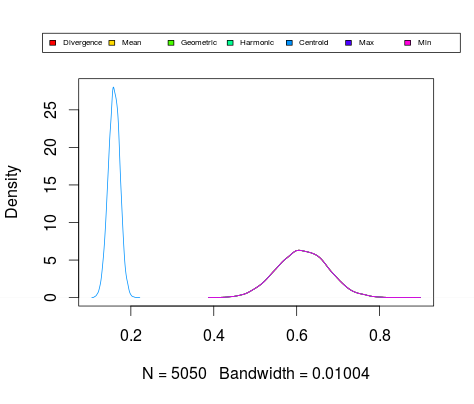
\includegraphics[width=0.5\textwidth]{gfx/correlations/2.png}
                \label{fig:triples}
        }%
        ~ %add desired spacing between images, e. g. ~, \quad, \qquad etc.
          %(or a blank line to force the subfigure onto a new line)
        \subfloat[5-tuples with mean euclidean distance to a centroid]{
                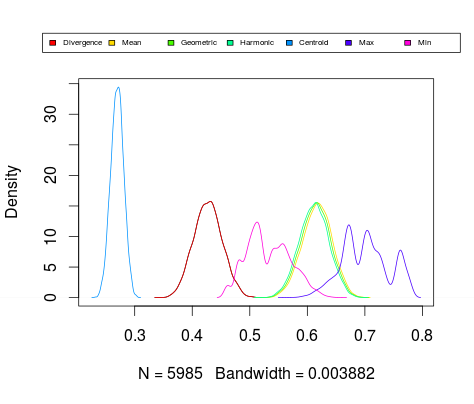
\includegraphics[width=0.5\textwidth]{gfx/correlations/4.png}
                \label{fig:5-tuples}
        }
        
        \subfloat[5-tuples with mean euclidean distance to a centroid]{
                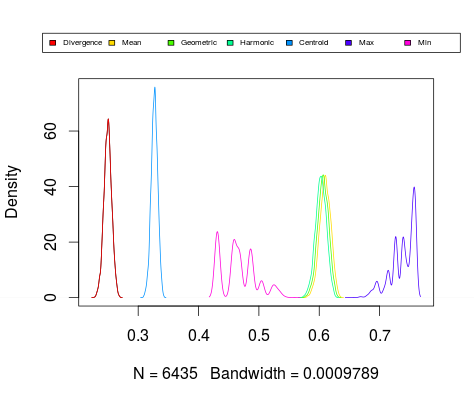
\includegraphics[width=0.5\textwidth]{gfx/correlations/8.png}
                \label{fig:5-tuples}
        }
        ~
        \subfloat[5-tuples with mean euclidean distance to a centroid]{
                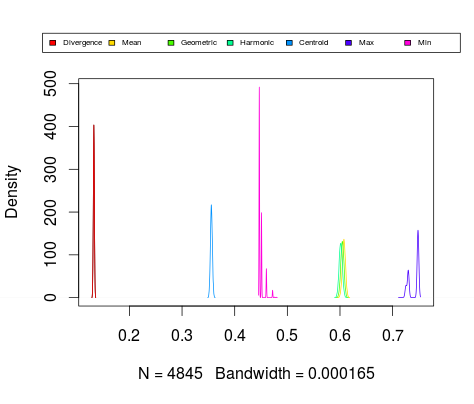
\includegraphics[width=0.5\textwidth]{gfx/correlations/16.png}
                \label{fig:5-tuples}
        }

        \caption[Correlation with divergence in 15-dimensional space]{Correlation with divergence in 15-dimensional space}\label{fig:corr-mean}
\end{figure}
%We compared our function to three other measures of multi-way divergence, based both on the SED metric and also on Euclidean distance. Set sizes of 3, 4 and 5 were chosen over randomly generated 5 and 15 dimensional probability vectors.  
%\begin{table}
% 
%\centering
%\begin{tabularx}{0.95\linewidth}{X l l l}
%\toprule
%\multicolumn{3}{r}{PCC} \\
%\cmidrule(r){2-4}
%5 dimension Structural entropic distance	& 3-tuple 	& 4-tuple 	& 5-tuple\\
%\midrule
%mean intra-cluster distance		& 0.991285		& 0.9918386		& 0.9943856\\
%mean distance to a centroid		& 0.9950909		& 0.9952373		& 0.9959319\\
%max intra-cluster distance		& 0.9365853		& 0.9027764		& 0.9021573\\	
%\midrule
%\multicolumn{3}{l}{5 dimension Euclidean distance} \\
%\midrule
%mean intra-cluster distance		& 0.9482936		& 0.9584011		& 0.9669735\\
%mean distance to a centroid		& 0.9478603		& 0.9565286		& 0.9634166\\
%max intra-cluster distance		& 0.9059921		& 0.8853846		& 0.8865668\\	
%\midrule
%\multicolumn{3}{l}{15 dimension Structural entropic distance} \\
%\midrule
%mean intra-cluster distance		& 0.9924866		& 0.990572		& 0.9915913\\
%mean distance to a centroid		& 0.9958805		& 0.9950946		& 0.9956354\\
%max intra-cluster distance		& 0.9166376		& 0.854482		& 0.8198081\\	
%\midrule
%\multicolumn{3}{l}{15 dimension Euclidean distance} \\
%\midrule
%mean intra-cluster distance		& 0.9645352		& 0.9657067		& 0.9677485\\
%mean distance to a centroid		& 0.964599		& 0.9649238		& 0.9662083\\
%max intra-cluster distance		& 0.8966909		& 0.8426229		& 0.8024388\\	
%\bottomrule
%\end{tabularx}
%\caption{Pearson's correlation coefficients for multi-way divergence}
%\label{term_table}
%\end{table}%
%The maximum distance within each cluster is taken by running through all pair-wise combinations and selecting the largest.  

The best correlation comes with the mean distance to a centroid.  This method is calculated by making a centroid using the mean vector then averaging all distances in the cluster to it.  Since multi-way divergence is a ratio of the complexity of a centroid to the geometric mean of individual complexities, there is much more in common with this definition.  Even when the comparison distance metric is Euclidean distance, a very strong correlation exists (figure \ref{fig:5-tuples}).

The mean intra-cluster distance also correlates well with multi-way divergence.  Figure \ref{fig:triples} shows the correlation with the mean intra-cluster distance, which appears to be strongest at the, more commonly used, lower end.  

Multi-way divergence correlates --  less strongly than the other methods -- with both SED and Euclidean maximum intra-cluster distance, and the correlation drops as the cluster size increases.  Rather than assessing the mutual similarity, the maximum distance simply describes the two farthest points in the cluster.  These two points must lie on the cluster perimeter and describe the spread of points across the space. Using only two points, however, fails to account for the spread in other dimensions, further verified by the drop in correlation in the higher dimensional space.
%\begin{figure}
%        \centering
%        \begin{subfigure}[b]{0.3\textwidth}
%                \centering
%				\includegraphics[width=\textwidth]{images/triples-max.png}
%                \caption{triples}
%                \label{fig:triples}
%        \end{subfigure}%
%        ~ %add desired spacing between images, e. g. ~, \quad, \qquad etc.
%          %(or a blank line to force the subfigure onto a new line)
%        \begin{subfigure}[b]{0.3\textwidth}
%                \centering
%                \includegraphics[width=\textwidth]{images/4-tuples-max.png}
%                \caption{4-tuples}
%                \label{fig:4-tuples}
%        \end{subfigure}
%        ~ %add desired spacing between images, e. g. ~, \quad, \qquad etc.
%          %(or a blank line to force the subfigure onto a new line)
%        \begin{subfigure}[b]{0.3\textwidth}
%                \centering
%                \includegraphics[width=\textwidth]{images/5-tuples-max.png}
%                \caption{5-tuples}
%                \label{fig:5-tuples}
%        \end{subfigure}
%        \caption{Correlations with maximum inter-cluster distance joining 15-dimensional spaces}\label{fig:corr-max}
%\end{figure}
\begin{figure}
        \centering
        \subfloat[triples with mean structural entropic distance]{
				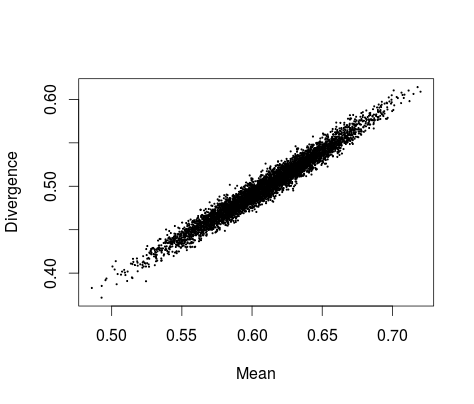
\includegraphics[width=0.5\textwidth]{gfx/correlations/3_mean.png}
                \label{fig:triples}
        }%
        ~ %add desired spacing between images, e. g. ~, \quad, \qquad etc.
          %(or a blank line to force the subfigure onto a new line)
        \subfloat[5-tuples with mean euclidean distance to a centroid]{
                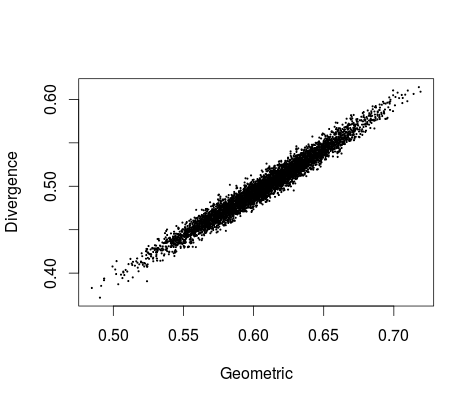
\includegraphics[width=0.5\textwidth]{gfx/correlations/3_geometric.png}
                \label{fig:5-tuples}
        }
        
        \subfloat[5-tuples with mean euclidean distance to a centroid]{
                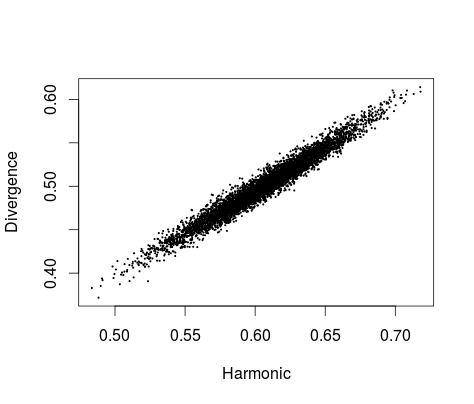
\includegraphics[width=0.5\textwidth]{gfx/correlations/3_harmonic.png}
                \label{fig:5-tuples}
        }
        ~
        \subfloat[5-tuples with mean euclidean distance to a centroid]{
                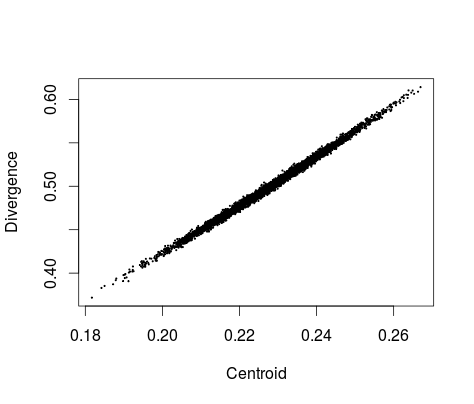
\includegraphics[width=0.5\textwidth]{gfx/correlations/3_centroid.png}
                \label{fig:5-tuples}
        }
                
        \subfloat[5-tuples with mean euclidean distance to a centroid]{
                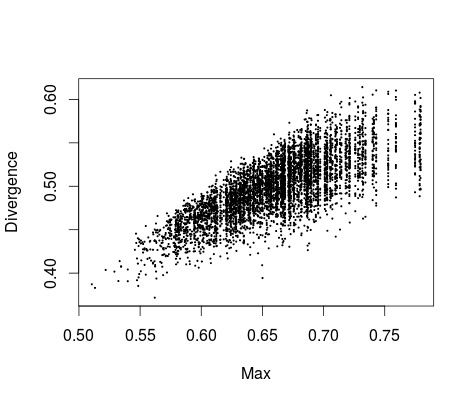
\includegraphics[width=0.5\textwidth]{gfx/correlations/3_max.png}
                \label{fig:5-tuples}
        }
        ~
        \subfloat[5-tuples with mean euclidean distance to a centroid]{
                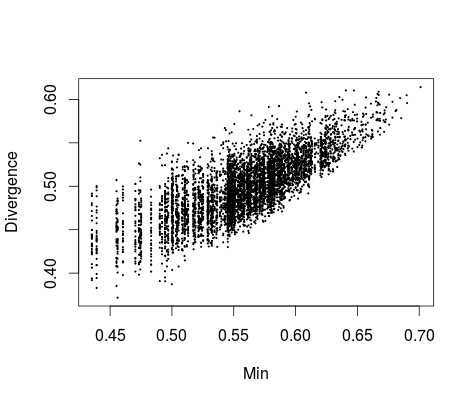
\includegraphics[width=0.5\textwidth]{gfx/correlations/3_min.png}
                \label{fig:5-tuples}
        }

        \caption[Correlation with divergence in 15-dimensional space]{Correlation with divergence in 15-dimensional space}\label{fig:corr-mean}
\end{figure}

\begin{figure}
        \centering
        \subfloat[triples with mean structural entropic distance]{
				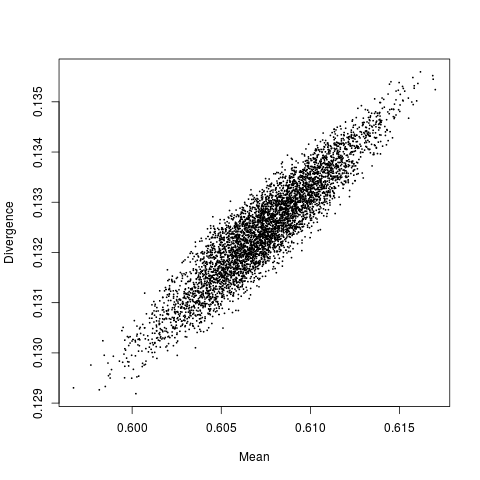
\includegraphics[width=0.5\textwidth]{gfx/correlations/16_Mean.png}
                \label{fig:triples}
        }%
        ~ %add desired spacing between images, e. g. ~, \quad, \qquad etc.
          %(or a blank line to force the subfigure onto a new line)
        \subfloat[5-tuples with mean euclidean distance to a centroid]{
                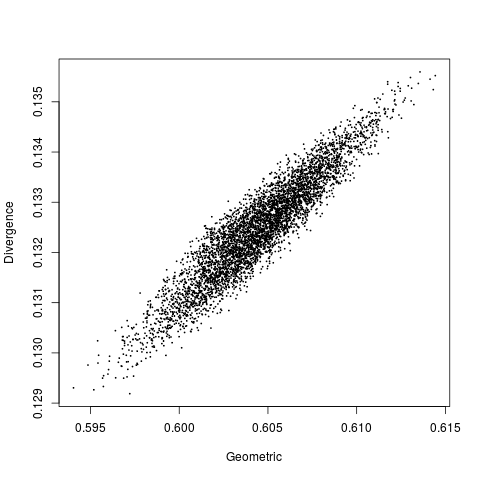
\includegraphics[width=0.5\textwidth]{gfx/correlations/16_Geometric.png}
                \label{fig:5-tuples}
        }
        
        \subfloat[5-tuples with mean euclidean distance to a centroid]{
                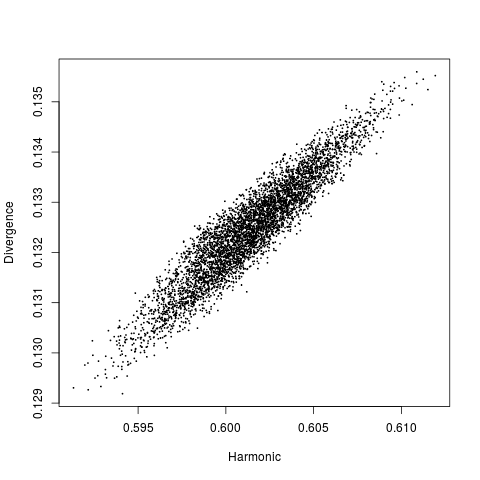
\includegraphics[width=0.5\textwidth]{gfx/correlations/16_Harmonic.png}
                \label{fig:5-tuples}
        }
        ~
        \subfloat[5-tuples with mean euclidean distance to a centroid]{
                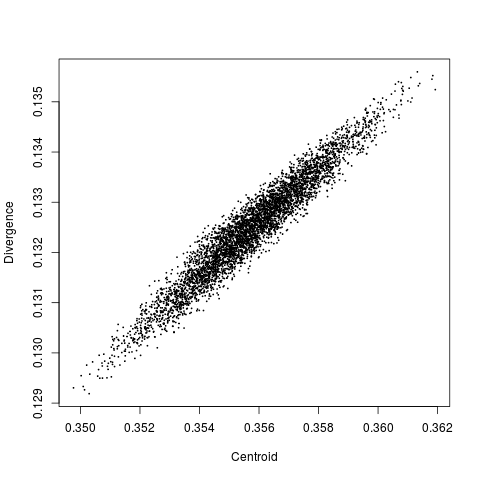
\includegraphics[width=0.5\textwidth]{gfx/correlations/16_Centroid.png}
                \label{fig:5-tuples}
        }
                
        \subfloat[5-tuples with mean euclidean distance to a centroid]{
                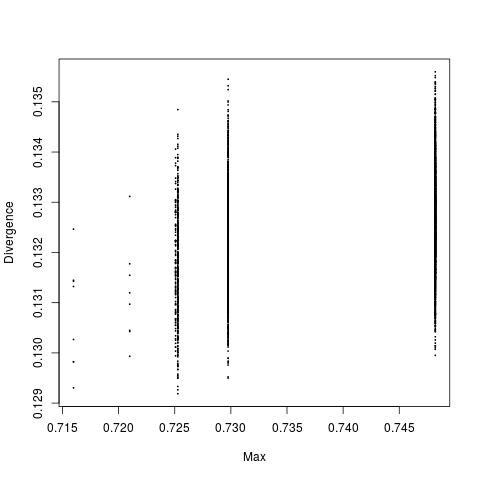
\includegraphics[width=0.5\textwidth]{gfx/correlations/16_Max.png}
                \label{fig:5-tuples}
        }
        ~
        \subfloat[5-tuples with mean euclidean distance to a centroid]{
                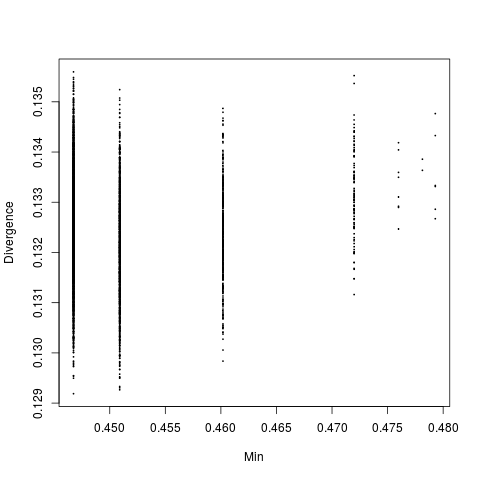
\includegraphics[width=0.5\textwidth]{gfx/correlations/16_Min.png}
                \label{fig:5-tuples}
        }

        \caption[Correlation with divergence in 15-dimensional space]{Correlation with divergence in 15-dimensional space}\label{fig:corr-mean}
\end{figure}

\begin{figure}
        \centering
        \subfloat[triples with mean structural entropic distance]{
				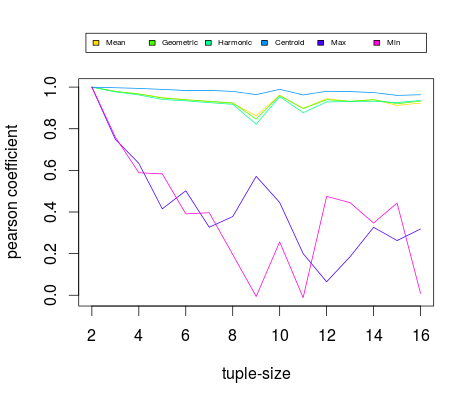
\includegraphics[width=0.5\textwidth]{gfx/correlations/pearson.png}
                \label{fig:triples}
        }%
        ~ %add desired spacing between images, e. g. ~, \quad, \qquad etc.
          %(or a blank line to force the subfigure onto a new line)
        \subfloat[5-tuples with mean euclidean distance to a centroid]{
                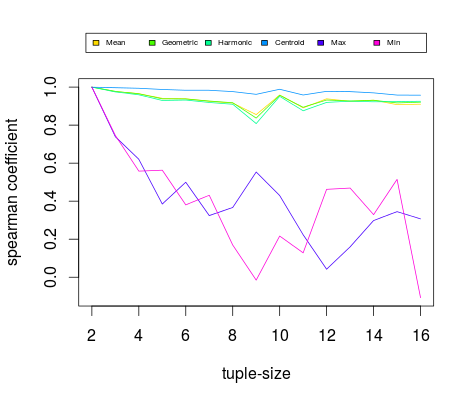
\includegraphics[width=0.5\textwidth]{gfx/correlations/spearman.png}
                \label{fig:5-tuples}
        }
        
        \subfloat[5-tuples with mean euclidean distance to a centroid]{
                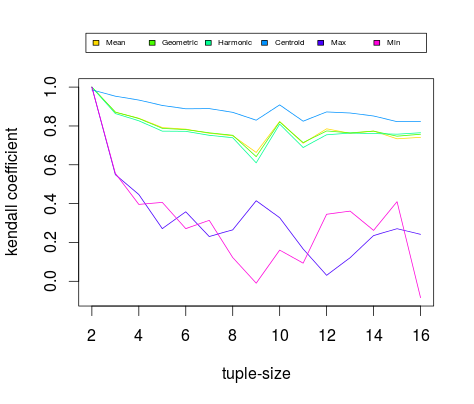
\includegraphics[width=0.5\textwidth]{gfx/correlations/kendall.png}
                \label{fig:5-tuples}
        }

        \caption[Correlation with divergence in 15-dimensional space]{Correlation with divergence in 15-dimensional space}\label{fig:corr-mean}
\end{figure}

%\section{Performance}
%When many calculations are performed over a given metric space, the complexity of individual vectors need only be calculated once and stored for later use, thus amortising the  cost of the calculation when multiple calls to divergence are required. The only calculation required is the complexity of the centroid, followed by some simple arithmetic, making the calculation really quite cheap.
%
%The performance of all the metrics depends on the number of distance calls required: divergence is constant, mean distance to centroid is linear, and mean distance is quadratic. We measured this to see the practical impact, Figure \ref{fig:performance} shows the time in nanoseconds to evaluate each function.  The mean inter-cluster distance is an order of magnitude slower than divergence when the set size is just 5. 

%\begin{figure}
%        \centering
%        \subfloat[Performance vs SED]{
%				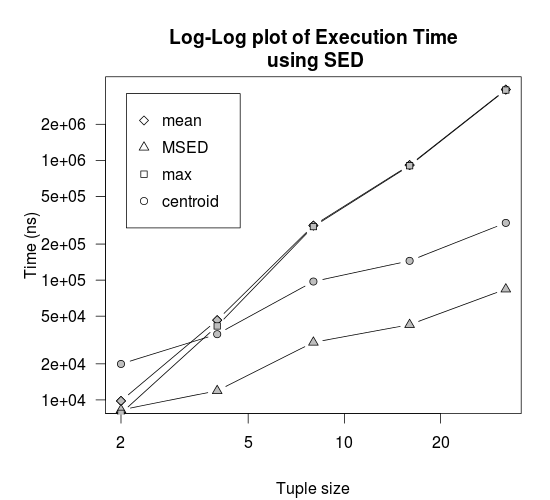
\includegraphics[width=0.5\textwidth]{gfx/sed_times.png}
%                \label{fig:triples}
%        }%
%        ~ %add desired spacing between images, e. g. ~, \quad, \qquad etc.
%          %(or a blank line to force the subfigure onto a new line)
%        \subfloat[Performance vs Euclidean Distance]{
%                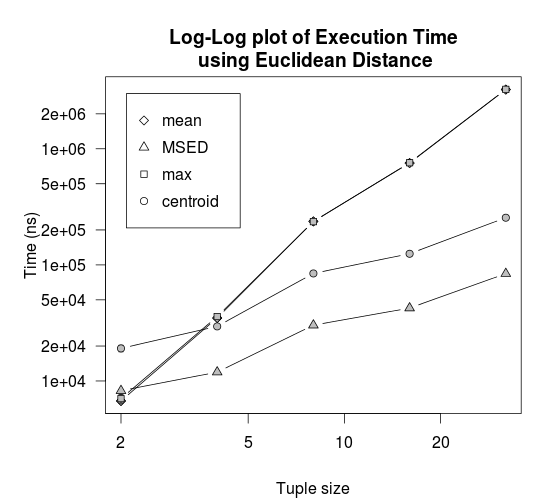
\includegraphics[width=0.5\textwidth]{gfx/euc_times.png}
%                \label{fig:5-tuples}
%        }
%
%        \caption[Performance]{Performance}\label{fig:msed_performance}
%\end{figure}

%We have recently made the observation that the function we had derived as a  distance function $d$ can be logically generalised to a definition over multiple operands; that is, it is a special case of a more general  function $D$ over a set of ensembles, such that $d(e_1,e_2) = D(\{e_1,e_2\})$.
%
%Our original ensemble distance is defined in terms of complexity and merge functions  ($C$ and $M$ respectively) over ensembles as follows:
%\[
%d(e_1,e_2) = \frac{C(M(e_1,e_2))}{\sqrt{C(e_1) \cdot C(e_2)}} - 1
%\]
%%
%The notional merge operator%
%\footnote{the name derives from ensembles used to model structured data}  is  an averaging operation over  ensembles:  $M(e_1,e_2)$ forms a new ensemble, with events drawn from $e_1 \cup e_2$, each assigned the  mean  probability of that event in $e_1$ and $e_2$. The complexity function $C(e)$ is $x^{H_x(e)}$ where $H_x(e)$ is the Shannon entropy \cite{}%
%\footnote{\cite{} gives much deeper mathematical insight of great value in this context} of the ensemble $e$ using base $x$ logarithms.  
%
%Our primary observation is that the semantics underlying the derivation of this form can be generalised to a set $E$ of ensembles, with $n$ elements denoted by $e_i$:
%%
%\[
%D(E) = \left(\frac{C(M'(E))}{\sqrt[n]{ \prod_i {C(e_i) }}} - 1\right) \cdot \frac{1}{n-1}
%\]
%%
%from which  it can be seen how the special case of $n=2$ reverts to the original distance function.
\section{Summary}
%
%************************************************
\chapter{Efficient Evaluation}\label{ch:efficient_evaluation}
%************************************************

In this chapter, we derive an equivalent metric first with the standard two-way SED using only intersecting 
dimensions to significantly reduce its cost, and secondly, generalising to the multi-way MSED whereby if there are $n$ input vectors we only need to consider dimensions that are non-zero in $> 1$ of the input vectors, avoiding the cost of calculating logs.  

We evaluate over both sparse vectors and inverted indices which allow parallel evaluation over large data spaces.  We show that a lower bound can be efficiently maintained during calculation so that the calculation may be eagerly abandoned.
\section{Avoiding calculation of the mean}
We consider the efficient evaluation of JSD, since it can be used in the calculation of MSED.  In particular, we are interested in an incremental evaluation since evaluation over large collections can be achieved through the use of an inverted index data structure, saving space.
\subsection{2-way case}
Although it appears that JSD requires the construction of a new vector $\mathbf{z}$, in fact, $\mathbf{z}$ does not need to be constructed.  Working with the vector notation from section \ref{vector_space} we can see this as follows
\begin{align}
    JSD(\mathbf{x}, \mathbf{y}) &= H_b(\mathbf{z}) - \frac{1}{2}(H_b(\mathbf{x}) + H_b(\mathbf{y}))\\
    &= -\sum_i z_i \log_b z_i - \frac{1}{2}(-\sum_i  x_i \log_b x_i - \sum_i  y_i \log_b y_i)\\
    &= -\frac{1}{2}\sum_i 2 \cdot z_i \log_b z_i - (x_i \log_b x_i + y_i \log_b y_i)\\
    &= \frac{1}{2}\sum_i  x_i \log_b x_i + y_i \log_b y_i  - (x_i+y_i) \log_b \frac{(x_i+y_i)}{2}
\end{align}  
%
avoiding the construction of $\mathbf{z}$.

Using base 2 logs allows the elimination of yet more terms:
%
\begin{align}
JSD(\mathbf{x}, \mathbf{y}) &= \frac{1}{2}\sum_i  x_i \log_2 x_i + y_i \log_2 y_i - (x_i+y_i)(\log_2 (x_i+y_i) - 1)\\
 &= \frac{1}{2}\sum_i  x_i \log_2 y_i  + x_i \log_2 y_i - (x_i+y_i) \log_2 (x_i+y_i) + x_i+y_i
\intertext{and, since $\sum_i x_i = \sum_i y_i=1$,}
JSD(\mathbf{x}, \mathbf{y}) &= 1 + \frac{1}{2}\sum_i  x_i \log_2 x_i + y_i \log_2 y_i - (x_i+y_i) \log_2 (x_i+y_i)
\intertext{Since we are interested in the incremental evaluation, we negate the summand function and name it:}
\F(x,y) &= (x+y) \log_2 (x+y) - x \log_2 x  - y \log_2 y
\intertext{giving:}
JSD(\mathbf{x}, \mathbf{y}) &= 1 - \frac{1}{2}\sum_i  \F(x_i,y_i)
\end{align}
where if either (or both) of $x_i$ or $y_i$ is equal to zero then so is $\F(x_i,y_i)$, thus only the non-zero intersection is required; that is, $\F(x_i,y_i)$ need only be evaluated when $x_i \neq 0$ and $y_i \neq 0$. 
%Evaluation over large collections can be achieved through the use of an inverted index data structure, saving space as well.
\begin{figure}
  \centering
  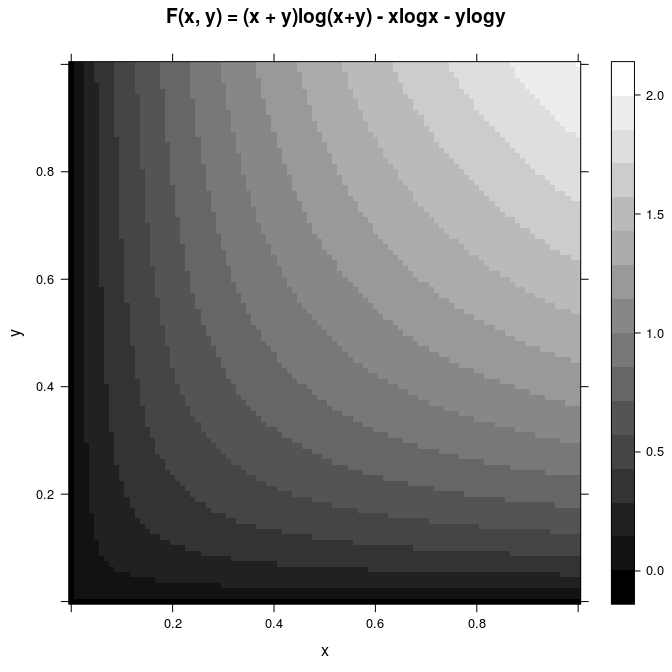
\includegraphics[width=4in]{gfx/F(x,y)}
  \caption[The function $\F$ on all possible inputs]
   {The function $\F$ on all possible inputs}
   \label{fig:F}
\end{figure}

\subsection{multi-way case}
In the multi-way case we follow the same reasoning.  Starting with the definition of $JSD$ we avoid the construction of $\mathbf{z}$ as follows:
%Although it appears that JSD requires the construction of a new vector $\mathbf{z}$, in fact, $\mathbf{z}$ does not need to be constructed.  Working with the vector notation from section \ref{vector_space} we can see this as follows
\begin{align}
    JSD(\mathbf{x}^{(1)}, \ldots, \mathbf{x}^{(n)}) &= H_b(\mathbf{z}) - \frac{1}{n}(\sum_j H_b(\mathbf{x}^{(j)}))\\
    &= -\sum_i z_i \log_b z_i - \frac{1}{n}(\sum_j -\sum_i  x^{(j)}_i \log_b x^{(j)}_i)\\
    &= -\frac{1}{n}\sum_i n \cdot z_i \log_b z_i - (\sum_j x^{(j)}_i \log_b x^{(j)}_i )\\
    &= \frac{1}{n}\sum_i  (\sum_j x^{(j)}_i \log_b x^{(j)}_i )  - (\sum_j x^{(j)}_i) \log_b \frac{(\sum_j x^{(j)}_i)}{n}
\end{align}  
%

This time using base $n$ logs allows the elimination of extra terms:
%
\begin{align}
JSD(\mathbf{x}^{(1)}, \ldots, \mathbf{x}^{(n)}) &= \frac{1}{n}\sum_i   (\sum_j x^{(j)}_i \log_n x^{(j)}_i ) - (\sum_j x^{(j)}_i) (\log_n \sum_j x^{(j)}_i - 1)\\
 &= \frac{1}{n}\sum_i (\sum_j x^{(j)}_i \log_n x^{(j)}_i ) - (\sum_j x^{(j)}_i) \log_n (\sum_j x^{(j)}_i) + (\sum_j x^{(j)}_i)
\intertext{and, since $\sum_i x^{(j)}_i = \sum_i x^{(k)}_i=1$, for any j, k}
JSD(\mathbf{x}^{(1)}, \ldots, \mathbf{x}^{(n)}) &= 1 + \frac{1}{n}\sum_i  (\sum_j x^{(j)}_i \log_n x^{(j)}_i ) -  (\sum_j x^{(j)}_i) \log_n (\sum_j x^{(j)}_i)
\intertext{again, we are interested in the incremental evaluation, so we generalise the $\F$ function from the 2-way case:}
\F(x^{(1)}, \ldots, x^{(n)}) &= (\sum_j x^{(j)}) \log_n (\sum_j x^{(j)}) - (\sum_j x^{(j)} \log_n x^{(j)})
\intertext{giving:}
JSD(\mathbf{x}^{(1)}, \ldots, \mathbf{x}^{(n)}) &= 1 - \frac{1}{n}\sum_i  \F(x^{(1)}_i,\ldots,x^{(n)}_i)
\end{align}
As before, we notice that $\F$ is equal to zero when $n - 1$ or more of the $n$ input values is zero.  Thus, we can avoid the expensive calculation of the logs and replace it with the cheaper count of zeros.
\section{Early termination}
%
The outcome of the metric, with range queries in similarity search, is of no interest if it is greater than the threshold $r$. We now show a way of optimising the calculation further.

The threshold requirement is written
\begin{align}
&&            &\frac{n^{1 - \frac{1}{n}\sum_{i = 1}^n  \F(x^{(1)}_i,\ldots, x^{(n)}_i)} - 1}{n - 1}   & \leq & & &r\\
&\Rightarrow& &n^{1 - \frac{1}{n}\sum_{i = 1}^n  \F(x^{(1)}_i,\ldots, x^{(n)}_i)} - 1   & \leq & & &(n - 1)r\\
&\Rightarrow& &1 - \frac{1}{n} \sum_{i = 1}^n  \F(x^{(1)}_i,\ldots, x^{(n)}_i)          & \leq & & &\log_n((n - 1)r + 1)\\
&\Rightarrow& &- \frac{1}{n} \sum_{i = 1}^n  \F(x^{(1)}_i,\ldots, x^{(n)}_i)          & \leq & & &\log_n((n - 1)r + 1) - 1\\	
&\Rightarrow& &\sum_{i = 1}^n  \F(x^{(1)}_i,\ldots, x^{(n)}_i)                          & \geq & & &n -  n\log_n((n - 1)r + 1)	
\end{align}
$\F$ can be seen as a similarity accumulator, and the term $n\log_n((n - 1)r + 1)$ as the maximum shortfall that may occur in order for the threshold $r$ not to be exceeded. 

If, at any point of the iterative calculation, we can determine that it is impossible for the value of $\sum_{i = 1}^n  \F(x^{(i)},\ldots, x^{(n)})$ to reach the threshold of $n -  n\log_n((n - 1)r + 1)$, then the calculation may be abandoned.

\begin{figure}
  \centering
  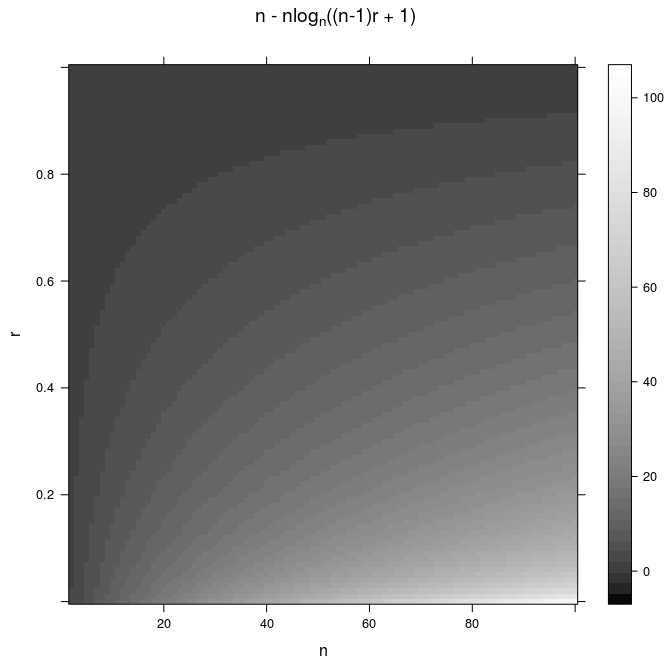
\includegraphics[width=4in]{gfx/threshold}
  \caption[Similarity lower bounds]
   {Similarity lower bounds}
   \label{fig:threshold}
\end{figure}

We calculate an upper bound for $\sum_{i = 1}^n  \F(x^{(i)},\ldots, x^{(n)})$ after $k$ stages of the iteration by consideration of the sum of terms:
\begin{equation}
\sum_{i = 1}^n  \F(x^{(i)},\ldots, x^{(n)}) = \sum_{i = 1}^k  \F(x^{(i)},\ldots, x^{(n)}) + \sum_{i = k+1}^n  \F(x^{(i)},\ldots, x^{(n)})
\end{equation}
At stage $k$, the value of the left hand term is known, and using the Jensen inequality we can calculate an upper bound for the right-hand term:
\begin{align}\label{equation_threshold}
&& &\sum_{i=k+1}^n  \F(x^{(i)},\ldots, x^{(n)}) & \le & &  &\F\left(\sum_{i=k+1}^n x^{(1)}_i,\ldots,\sum_{i=k+1}^n x^{(n)}_i\right)\\
&\Rightarrow& &\sum_{i=k+1}^n  \F(x^{(i)},\ldots, x^{(n)}) & \le & & &\F\left(1 - \sum_{i=1}^k x^{(1)}_i,\ldots, 1 - \sum_{i=1}^k x^{(n)}_i \right)
\end{align}
without knowledge of even the number of dimensions still to be computed.

Thus if at any stage $k$ the inequality
\begin{equation}
\sum_{i = 1}^k  \F(x^{(i)},\ldots, x^{(n)}) + \F\left(1 - \sum_{i=1}^k x^{(1)}_i,\ldots, 1 - \sum_{i=1}^k x^{(n)}_i \right) < n -  n\log_n((n - 1)r + 1)
\end{equation}
becomes true the calculation may be terminated early with the knowledge that the distance falls out with the range of the query.

Whether the optimisation based on this observation is worth applying or not depends entirely on the context of the calculation; it requires the calculation of an extra application of $\F$ and, if applied at each stage of the calculation, would only be cost-effective if a saving equivalent to half the number of stages was achieved. This is not to say that the observation is of no use, and in particular there may be circumstances where an I/O saving can be achieved.

%--------------------------------------------------------------------------------------------------%	
\section{Evaluation}
\label{section_evaluation}
Based on the above algebraic observations, we implemented five different methods of evaluating the metric, as follows.  All of which avoided the calculation of the mean vector:

\begin{singlespace*} 
\begin{description}\item[Inverted Index] Using an inverted index (skipping dimensions where > n-1 values are 0);
\item[Inverted Index ET] using an inverted index with early termination (skipping dimensions where > n-1 values are 0).
\item[Sparse Vectors] All dimensions of the vectors being compared are accessed;
\item[Sparse Vectors 2] skipping dimensions where > n-1 values are 0;
\item[Sparse Vectors 3] skipping dimensions where > n-1 values are 0, with early termination;
\end{description}
\end{singlespace*}
\begin{figure}[h!]
\centering
\subfloat[Simple Vector Representation] 
{\label{fig:simple_vector_representation}
%%
% Dense vectors
%%
\begin{tikzpicture}
\node[rotate=90] at (-0.75, 1.5) {Vector Id};
\node [left] at (-0.1, 2) {0};
\node [left] at (-0.1, 1.5) {1};
\node [left] at (-0.1, 1) {2};

\node at (2.75, 3.5){Dimension};
\node at (2, 3) {0};
\node at (2.5, 3) {1};
\node at (3, 3) {2};
\node at (3.5, 3) {3};

\draw [help lines, step=0.5,xshift=0cm,yshift=0.75cm] (0,0) grid (0.5,1.5);
\draw[thick,->] (0.5,1) -- (1.75,0.5);
\draw[thick,->] (0.5,1.5) -- (1.75,1.5);
\draw[thick,->] (0.5,2) -- (1.75,2.5);

\draw [help lines, step=0.5,xshift=-0.25cm,yshift=0.25cm] (2 - 0.002, 2 - 0.002) grid +(2.002,0.5+0.002);
\foreach \x/\y/\z in {2/2.5/0.3, 2.5/2.5/0, 3/2.5/0, 3.5/2.5/0.7}
	\node[font=\small] at (\x, \y) {\z};

\draw [help lines, step=0.5,xshift=-0.25cm,yshift=-0.75cm] (2 - 0.002, 2 - 0.002) grid +(2.002,0.5+0.002);
\foreach \x/\y/\z in {2/1.5/0, 2.5/1.5/0.1, 3/1.5/0, 3.5/1.5/0.9}
	\node[font=\small] at (\x, \y) {\z};
	
\draw [help lines, step=0.5,xshift=-0.25cm,yshift=-1.75cm] (2 - 0.002, 2 - 0.002) grid +(2.002,0.5+0.002);
\foreach \x/\y/\z in {2/0.5/0.4, 2.5/0.5/0.6, 3/0.5/0, 3.5/0.5/0}
	\node[font=\small] at (\x, \y) {\z};
\end{tikzpicture}
} \quad
\subfloat[Sparse Vector Representation] 
{\label{fig:sparse_vector_representation}
%%
% Sparse vectors
%%
\begin{tikzpicture}
\node[rotate=90] at (-0.75, 1.5) {Vector Id};
\node [left] at (-0.1, 2) {0};
\node [left] at (-0.1, 1.5) {1};
\node [left] at (-0.1, 1) {2};

\node at (2.75, 3.5){Dimension Id / Value};

\draw [help lines, step=0.5,xshift=0cm,yshift=0.75cm] (0,0) grid (0.5,1.5);
\draw[thick,->] (0.5,1) -- (1.75,0.25);
\draw[thick,->] (0.5,1.5) -- (1.75,1.5);
\draw[thick,->] (0.5,2) -- (1.75,2.75);

\draw [help lines, step=1,xshift=-0.25cm,yshift=0.25cm] (2 - 0.002, 2 - 0.002) grid +(2.002,1+0.002);
\draw [help lines, step=0.5,xshift=-0.25cm,yshift=0.5cm] (2 - 0.002, 2 - 0.002) grid +(2.002,0.5+0.002);
\foreach \x/\y/\z in {2/2.75/0, 2.5/2.75/0.3, 3/2.75/3, 3.5/2.75/0.7}
	\node[font=\small] at (\x, \y) {\z};

\draw [help lines, step=1,xshift=-0.25cm,yshift=-1cm] (2 - 0.002, 2 - 0.002) grid +(2.002,1+0.002);
\draw [help lines, step=0.5,xshift=-0.25cm,yshift=-0.75cm] (2 - 0.002, 2 - 0.002) grid +(2.002,0.5+0.002);
\foreach \x/\y/\z in {2/1.5/1, 2.5/1.5/0.1, 3/1.5/3, 3.5/1.5/0.9}
	\node[font=\small] at (\x, \y) {\z};
	
\draw [help lines, step=1,xshift=-0.25cm,yshift=-2.25cm] (2 - 0.002, 2 - 0.002) grid +(2.002,1+0.002);
\draw [help lines, step=0.5,xshift=-0.25cm,yshift=-2cm] (2 - 0.002, 2 - 0.002) grid +(2.002,0.5+0.002);
\foreach \x/\y/\z in {2/0.25/0, 2.5/0.25/0.4, 3/0.25/1, 3.5/0.25/0.6}
	\node[font=\small] at (\x, \y) {\z};
\end{tikzpicture}
} \quad
\subfloat[Inverted Index Representation] 
{\label{fig:inverted_index_representation}

%%
% Inverted Index
%%
\begin{tikzpicture}
\node[rotate=90] at (-0.3, 1.5) {Dimension Id};
\node [left] at (0.5, 2.5) {0};
\node [left] at (0.5, 1.5) {1};
\node [left] at (0.5, 0.5) {3};

\node at (3, 3.5){Vector Id / Value};

\draw [help lines, step=1,xshift=0cm,yshift=0cm] (0,0) grid (1,3);
\draw [help lines, step=0.5,xshift=0cm,yshift=0.25cm] (0,0) grid (1,0.5);
\draw [help lines, step=0.5,xshift=0cm,yshift=1.25cm] (0,0) grid (1,0.5);
\draw [help lines, step=0.5,xshift=0cm,yshift=2.25cm] (0,0) grid (1,0.5);
\draw[thick,->] (1,0.5) -- (2.25,0.25);
\draw[thick,->] (1,1.5) -- (2.25,1.5);
\draw[thick,->] (1,2.5) -- (2.25,2.75);

\draw [help lines, step=1,xshift=0.25cm,yshift=0.25cm] (2 - 0.002, 2 - 0.002) grid +(2.002,1+0.002);
\draw [help lines, step=0.5,xshift=0.25cm,yshift=0.5cm] (2 - 0.002, 2 - 0.002) grid +(2.002,0.5+0.002);
\foreach \x/\y/\z in {2/2.75/0, 2.5/2.75/0.3, 3/2.75/3, 3.5/2.75/0.4}
	\node[font=\small,xshift=0.5cm] at (\x, \y) {\z};

\draw [help lines, step=1,xshift=0.25cm,yshift=-1cm] (2 - 0.002, 2 - 0.002) grid +(2.002,1+0.002);
\draw [help lines, step=0.5,xshift=0.25cm,yshift=-0.75cm] (2 - 0.002, 2 - 0.002) grid +(2.002,0.5+0.002);
\foreach \x/\y/\z in {2/1.5/1, 2.5/1.5/0.1, 3/1.5/3, 3.5/1.5/0.6}
	\node[font=\small,xshift=0.5cm] at (\x, \y) {\z};
	
\draw [help lines, step=1,xshift=0.25cm,yshift=-2.25cm] (2 - 0.002, 2 - 0.002) grid +(2.002,1+0.002);
\draw [help lines, step=0.5,xshift=0.25cm,yshift=-2cm] (2 - 0.002, 2 - 0.002) grid +(2.002,0.5+0.002);
\foreach \x/\y/\z in {2/0.25/0, 2.5/0.25/0.7, 3/0.25/3, 3.5/0.25/0.9}
	\node[font=\small,xshift=0.5cm] at (\x, \y) {\z};
\end{tikzpicture}
}
\caption[]{}
\end{figure}
A number of generated spaces were used to test the mechanisms.  The generator was set to populate sparse spaces of 50, 100, 200, 400, 800, 1600 and 3200 dimensions: 50 dimensions being populated in each.  We used two types of generator, which produced what we call either shuffled or unshuffled vectors.  In the unshuffled vectors, the generator populated the first 50 dimensions of each vector; in the shuffled vectors, the generator evenly distributed the populated dimensions among the $n$ dimensions by randomly shuffling the unshuffled vectors' dimensions. Search thresholds to return $10^{-4}$ of the data were then calculated for each space.
%For 50 dense dimensions, IDIM: x, with median distance of x. 
%\begin{figure}[h]
%\centering
%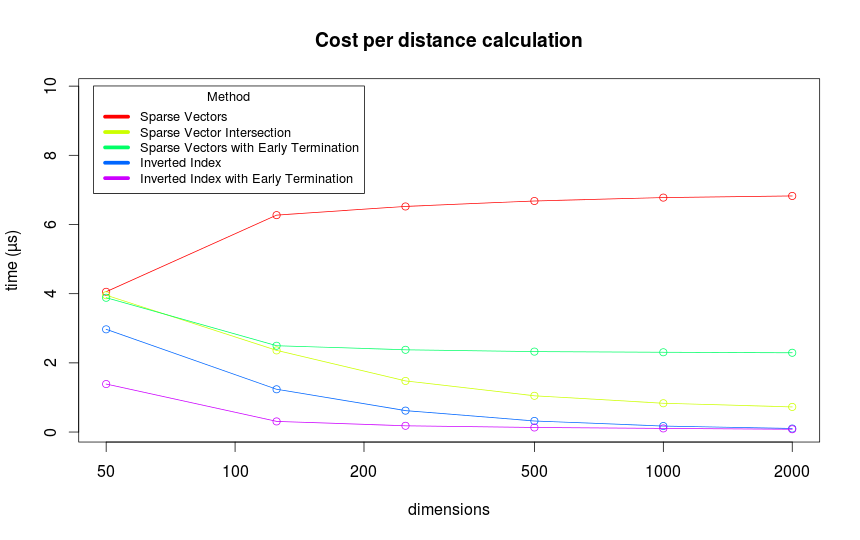
\includegraphics[width=0.9\columnwidth]{gfx/speedup_sed}
%\caption[Efficiency techniques]{distance times showing how the different techniques perform on increasingly sparse vectors}
%\label{fig:speedup_sed}
%\end{figure}

A metric index structure achieves no significant cost saving in these spaces; the space with 50 dense dimensions has an IDIM of x, with median distance of x.  IDIM increases, furthermore, with both the number of dimensions in the space and the relative sparsity.

Figure \ref{fig:sed_timings_shuffled} shows the effect of increasing the sparsity on shuffled vectors.  Initially, the sparse vectors are much quicker than the inverted index, but as the sparsity increases the inverted index becomes more efficient than the sparse vectors; this gap narrows, however, as the tuple size increases.  In all cases, the cost of maintaining the threshold invariant outweighs the saving from early termination.

\begin{figure}
        \centering
        \subfloat[2-tuple]{
				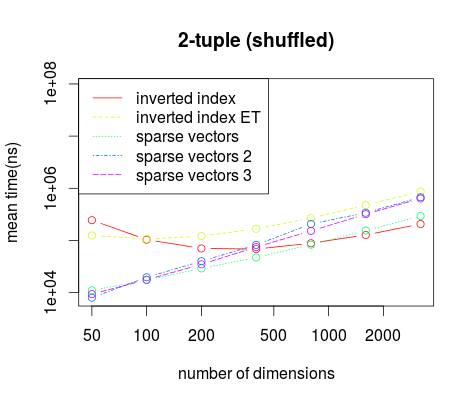
\includegraphics[width=0.35\textwidth]{gfx/times/shuffled/02.png}
                \label{fig:shuffled_02}
        }%
        ~ 
        \subfloat[4-tuple]{
				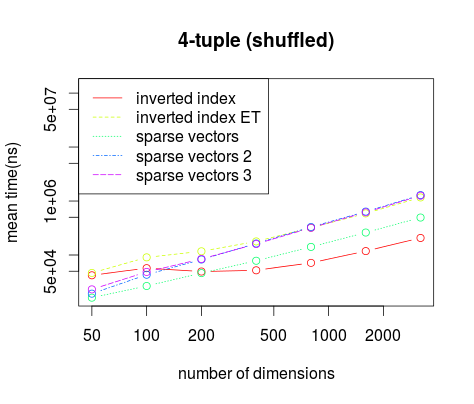
\includegraphics[width=0.35\textwidth]{gfx/times/shuffled/04.png}
                \label{fig:shuffled_04}
        }
        
         
        \subfloat[8-tuple]{
				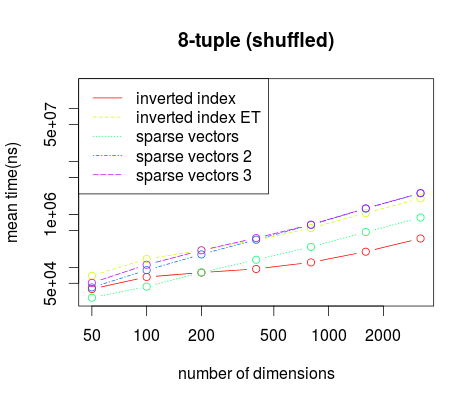
\includegraphics[width=0.35\textwidth]{gfx/times/shuffled/08.png}
                \label{fig:shuffled_08}
        }
        ~ 
        \subfloat[16-tuple]{
				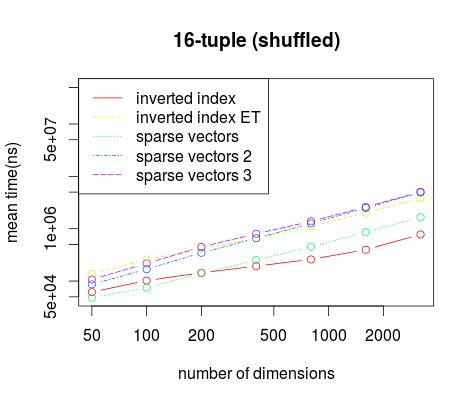
\includegraphics[width=0.35\textwidth]{gfx/times/shuffled/16.png}
                \label{fig:shuffled_16}
        }
    
        \caption[Comparison of evaluation techniques on the shuffled dataset over increasing sparsity]{Comparison of evaluation techniques on the shuffled datasets over increasing sparsity}\label{fig:sed_timings_shuffled}
\end{figure}

Figure \ref{fig:sed_timings_unshuffled} shows the effect of increasing the sparsity on unshuffled vectors.  With the 2-tuples shown in \ref{fig:unshuffled_02}, an inverted index is slower than the sparse vector representations, but benefits from using early termination.  The sparse vectors, also however, benefit significantly both from skipping dimensions and early termination.  As the tuple size is increased, the difference between sparse vectors and the inverted index narrows, and the inverted index even runs more efficiently beyond a certain point of sparsity.  Again, the higher tuple size show an impressive saving from early termination both in the inverted index and sparse vectors.   
\begin{figure}
        \centering
        \subfloat[2-tuple]{
				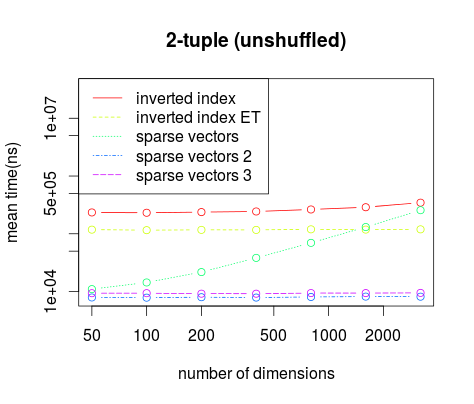
\includegraphics[width=0.35\textwidth]{gfx/times/unshuffled/02.png}
                \label{fig:unshuffled_02}
        }%
        ~ 
        \subfloat[4-tuple]{
				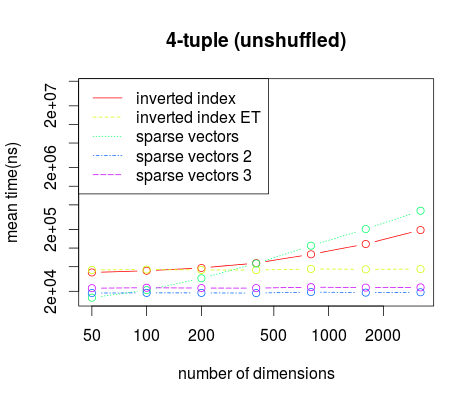
\includegraphics[width=0.35\textwidth]{gfx/times/unshuffled/04.png}
                \label{fig:unshuffled_04}
        }
        
         
        \subfloat[8-tuple]{
				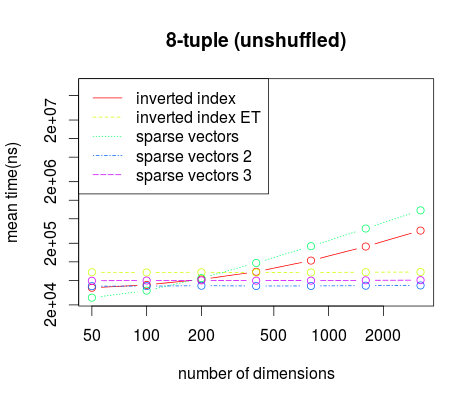
\includegraphics[width=0.35\textwidth]{gfx/times/unshuffled/08.png}
                \label{fig:unshuffled_08}
        }
        ~ 
        \subfloat[16-tuple]{
				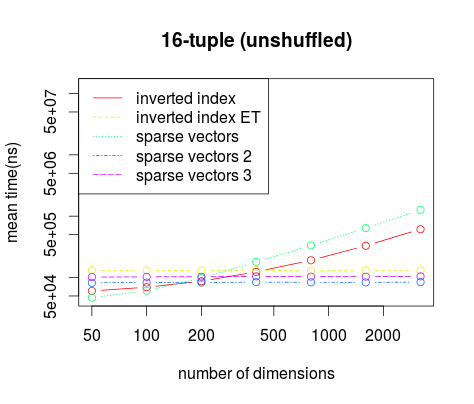
\includegraphics[width=0.35\textwidth]{gfx/times/unshuffled/16.png}
                \label{fig:unshuffled_16}
        }
    
        \caption[Comparison of evaluation techniques on the unshuffled dataset over increasing sparsity]{Comparison of evaluation techniques on the unshuffled datasets over increasing sparsity}\label{fig:sed_timings_unshuffled}
\end{figure}
% ------------------------------------------------------------------------------------------------------------------

Figure \ref{fig:sed_timings_techniques_shuffled} shows the growth of each mechanism on the shuffled data.  The growth of pattern is the same for all mechanisms: dense spaces show no extra cost when increasing the tuple size, but as the sparsity increases so does the rate of growth.
\begin{figure}
        \centering
        \subfloat[Inverted Index]{
				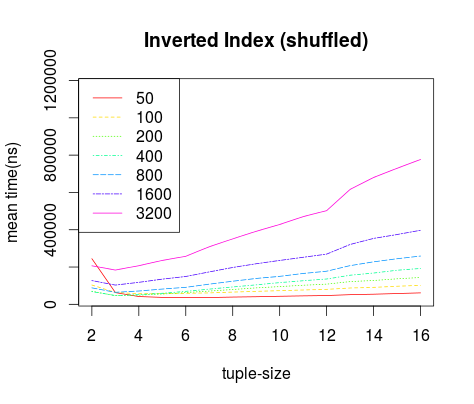
\includegraphics[width=0.35\textwidth]{gfx/times/shuffled/inverted_index.png}
                \label{fig:shuffled_inverted_index}
        }%
        ~ 
        \subfloat[Inverted Index ET]{
				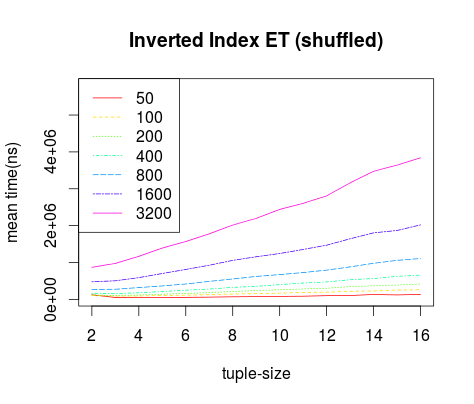
\includegraphics[width=0.35\textwidth]{gfx/times/shuffled/inverted_index_et.png}
                \label{fig:shuffled_inverted_index_et}
        }
        
         
        \subfloat[Sparse Vectors]{
				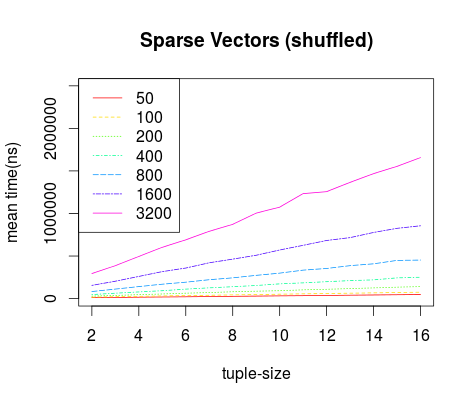
\includegraphics[width=0.35\textwidth]{gfx/times/shuffled/sparse_vectors.png}
                \label{fig:shuffled_sparse_vectors}
        }
        ~ 
        \subfloat[Sparse Vectors 2]{
				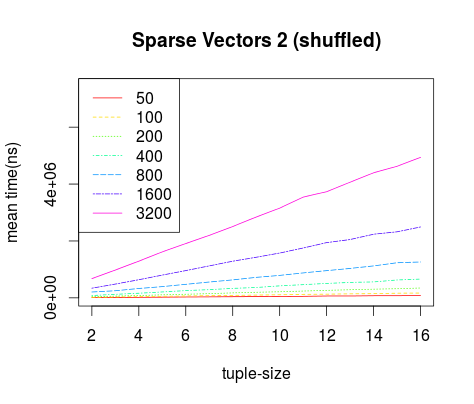
\includegraphics[width=0.35\textwidth]{gfx/times/shuffled/sparse_vectors_2.png}
                \label{fig:shuffled_sparse_vectors_2}
        }
        
        
        \subfloat[Sparse Vectors 3]{
				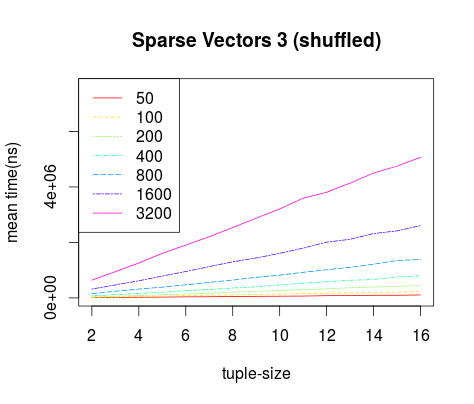
\includegraphics[width=0.35\textwidth]{gfx/times/shuffled/sparse_vectors_3.png}
                \label{fig:shuffled_sparse_vectors_3}
        }
    
        \caption[Effect of tuple size on the shuffled datasets for each of the evaluation techniques]{Effect of tuple size on the shuffled datasets for each of the evaluation techniques}\label{fig:sed_timings_techniques_shuffled}
\end{figure}

Figure \ref{fig:sed_timings_techniques_unshuffled} shows the growth of each mechanism on the unshuffled data.  The effect of early termination makes all levels of sparsity behave the same.  Whereas without early termination, the growth is larger for more sparse vectors.
\begin{figure}
        \centering
        \subfloat[Inverted Index]{
				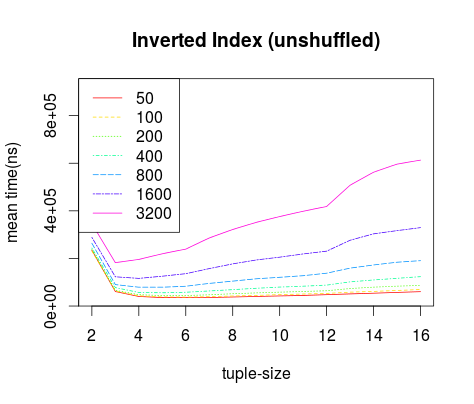
\includegraphics[width=0.35\textwidth]{gfx/times/unshuffled/inverted_index.png}
                \label{fig:unshuffled_inverted_index}
        }%
        ~ 
        \subfloat[Inverted Index ET]{
				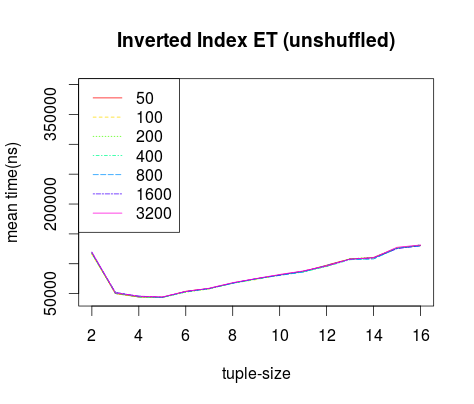
\includegraphics[width=0.35\textwidth]{gfx/times/unshuffled/inverted_index_et.png}
                \label{fig:unshuffled_inverted_index_et}
        }
        
         
        \subfloat[Sparse Vectors]{
				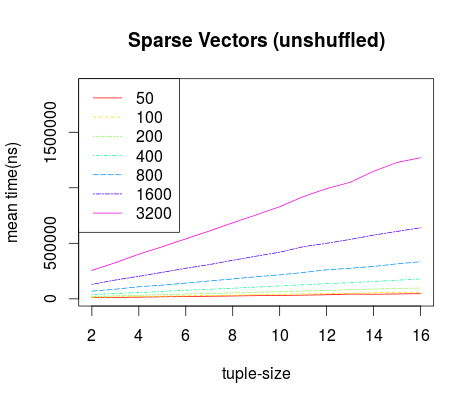
\includegraphics[width=0.35\textwidth]{gfx/times/unshuffled/sparse_vectors.png}
                \label{fig:unshuffled_sparse_vectors}
        }
        ~ 
        \subfloat[Sparse Vectors 2]{
				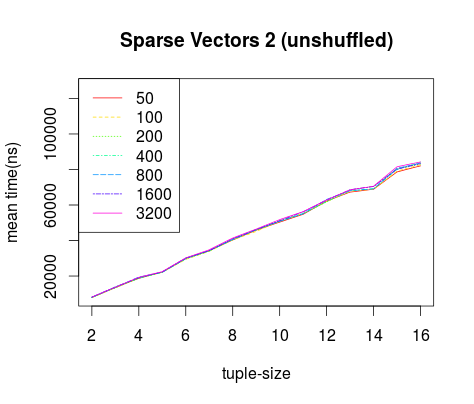
\includegraphics[width=0.35\textwidth]{gfx/times/unshuffled/sparse_vectors_2.png}
                \label{fig:unshuffled_sparse_vectors_2}
        }
        
        \subfloat[Sparse Vectors 3]{
				\includegraphics[width=0.35\textwidth]{gfx/times/unshuffled/sparse_vectors_3.png}
                \label{fig:unshuffled_sparse_vectors_3}
        }
    
        \caption[Effect of tuple size on the unshuffled datasets for each of the evaluation techniques]{Effect of tuple size on the unshuffled datasets for each of the evaluation techniques}\label{fig:sed_timings_techniques_unshuffled}
\end{figure}

% ------------------------------------------------------------------------------------------------------------------
Figure \ref{fig:sed_timings_dims_shuffled} compares the growth associated with increasing tuple size of each mechanism on the shuffled data.  On all levels of sparseness, using early termination increases the growth of cost associated with increasing the tuple size.
\begin{figure}
        \centering
        \subfloat[50 dims]{
				\includegraphics[width=0.35\textwidth]{gfx/times/shuffled/0050.png}
                \label{fig:shuffled_0050}
        }%
        ~ 
        \subfloat[100 dims]{
				\includegraphics[width=0.35\textwidth]{gfx/times/shuffled/0100.png}
                \label{fig:shuffled_0100}
        }
        
         
        \subfloat[200 dims]{
				\includegraphics[width=0.35\textwidth]{gfx/times/shuffled/0200.png}
                \label{fig:shuffled_0200}
        }
        ~ 
        \subfloat[400 dims]{
				\includegraphics[width=0.35\textwidth]{gfx/times/shuffled/0400.png}
                \label{fig:shuffled_0400}
        }
        
        
        \subfloat[800 dims]{
				\includegraphics[width=0.35\textwidth]{gfx/times/shuffled/0800.png}
                \label{fig:shuffled_0800}
        }
         ~ 
        \subfloat[1600 dims]{
				\includegraphics[width=0.35\textwidth]{gfx/times/shuffled/1600.png}
                \label{fig:shuffled_1600}
        }
        
        
        \subfloat[3200 dims]{
				\includegraphics[width=0.35\textwidth]{gfx/times/shuffled/3200.png}
                \label{fig:shuffled_3200}
        }
    
        \caption[shuffled]{Shuffled}\label{fig:sed_timings_dims_shuffled}
\end{figure}

Figure \ref{fig:sed_timings_dims_unshuffled} compares the growth associated with increasing the tuple size of each mechanism on unshuffled data.  In this case we see that early termination has a positive effect.  Those with early termination grow more quickly.
\begin{figure}
        \centering
        \subfloat[50 dims]{
				\includegraphics[width=0.35\textwidth]{gfx/times/unshuffled/0050.png}
                \label{fig:unshuffled_0050}
        }%
        ~ 
        \subfloat[100 dims]{
				\includegraphics[width=0.35\textwidth]{gfx/times/unshuffled/0100.png}
                \label{fig:unshuffled_0100}
        }
        
         
        \subfloat[200 dims]{
				\includegraphics[width=0.35\textwidth]{gfx/times/unshuffled/0200.png}
                \label{fig:unshuffled_0200}
        }
        ~ 
        \subfloat[400 dims]{
				\includegraphics[width=0.35\textwidth]{gfx/times/unshuffled/0400.png}
                \label{fig:unshuffled_0400}
        }
        
        \subfloat[800 dims]{
				\includegraphics[width=0.35\textwidth]{gfx/times/unshuffled/0800.png}
                \label{fig:unshuffled_0800}
        }
        ~ 
        \subfloat[1600 dims]{
				\includegraphics[width=0.35\textwidth]{gfx/times/unshuffled/1600.png}
                \label{fig:unshuffled_1600}
        }
        
        \subfloat[3200 dims]{
				\includegraphics[width=0.35\textwidth]{gfx/times/unshuffled/3200.png}
                \label{fig:unshuffled_3200}
        }    
        \caption[Unshuffled]{Unshuffled}\label{fig:sed_timings_dims_unshuffled}
\end{figure}
%IDIM and threshold values may not be useful characteristics of the space. 
%With 95\% sparsity, the data is likely unevenly distributed in the space; threshold search values may not be significantly greater than those in the dense space. Real data sets bear out this intuition: similar objects are still similar in absolute terms independent of the dimensions for which they have no value.

%\begin{figure}[h]
%\centering
%\includegraphics[width=0.9\columnwidth]{gfx/early_termination_thresholds}
%\caption[Early termination]{Cost of distance using early termination with thresholds $10^{-5}$ and $10^{-6}$}
%\label{fig:speedup_sed}
%\end{figure}

%For the dense benchmark set, definitions A, B and C gave almost the same times, which is unsurprising given there were no zero values. Exactly the same calculations took place in definitions A and B, while definition C produced a minor cost saving. This was further improved by the smaller threshold.  The saving by definition C was insignificant since the overhead of calculating the threshold values was almost as great.
%
%Definitions D and E gave a substantial saving, which is unexpected; definition D performed exactly the same set of calculations as definitions A and B. The only difference is the order in which the calculations were performed.  It may be the manner in which the data are fetched from slower to faster memory; inverted indices optimise this movement by moving the values in bigger chunks, allowing hardware optimisations to be used. While the movement here is between main and cache memory, the same principles apply with very large data sets between disk and main memory.
%
%Figure \ref{fig:speedup_sed} shows the threshold calculation of definition E was much more valuable in this context than its use in definition C. 
%While some of the calculation was amortised by the single traversal along the query vector; we do not fully understand the magnitude of the extra cost saving.
%
%%The trends as the overall dimensionality of the space increases fully vindicates our rationale. 
%As the overall dimensionality of the space was increased, definition A's times grew with the number of dimensions: first, the amount of data being moved through the processor memory increased; secondly, the rise in dimensions that have zero values in both operands yielded no extra saving.  As the size of the non-zero intersection diminished with increased sparsity, fewer calculations were performed by definition B, while the saving observed for definition C was lost; the cost of maintaining the threshold calculation outweighed the saving of early termination.  
%
%Although the same set of calculations were performed by definitions B and D, with definition D the volume of data passed though the processor cache decreased. The cost of maintaining the threshold calculation of Definition E, however, becomes proportionally greater, and since its advantage is increased with higher dimensionality, its relative advantage was lost.  It is still worth noting that, even at 2,000 dimensions, there was still a significant cost saving from this technique.
%
%Over the highest dimensions, a cost saving of almost two orders of magnitude was achieved, and the reasons for this should be maintained over very large data sets which are resident on disk rather than in memory.
\section{Conclusion}
The benefit associated with early termination and skipping dimensions clearly depends on the dataset being considered.  We examined the two extremes: when all the data have the same dimensions occupied and when they are populated randomly.  In the first instance, early termination clearly helped to reduce the cost of the calculation, but in the second the cost of maintaining the threshold calculation outweighed any saving.  In reality, most datasets will lie somewhere between these extremes, and may require some analysis to determine whether it would be appropriate to use these mechanisms.


\cleardoublepage
%
\ctparttext{%
%
Having explored the various properties of structural entropic distance we now shift our attention to the more practical aspect of applying it to common problems involving distance.%
%
}
%
\part{Applications of SED}
%
%************************************************
\chapter{Similarity Search}\label{ch:similarity_search}
%************************************************
\section{The cost of similarity search}
Having established the link between JSD and SED, we should now like to compare them.  Since both give the same ordering, we must examine efficiency.  We will compare them using intrinsic dimensionality (IDIM) and a probabilistic analysis designed to measure the cost and general notion of the tractability of similarity search techniques over high-dimensional metric spaces.  

Intrinsic dimensionality has been introduced as a tractability measure\cite{}, and a lower bound for index cost has been established. In practice, however, we have found different approximately-Gaussian distance distributions with the same IDIM may have very different probability densities close to the origin, and this has a far greater implication on performance than the IDIM. IDIM is really meaningful only within the context of a close-to-perfect Gaussian distribution, to which many metric/data combinations do not conform.

To address these limitations, we have constructed a methodology to perform a probabilistic analysis over metric spaces. Like IDIM, it is based
only on the distances over data, rather than the data itself. According to probability densities at both the median, and close to the origin. We show how this can be used to estimate the cost of a search operation over a given size of data.  It can be calculated via random sampling over a data set, and we have assessed performance predictions against measured performances on various data sets and found to be useful.

Many metric spaces over which similarity search is desirable suffer from the so-called curse of dimensionality. In the domain of Similarity Search, this refers to the effect whereby, as the number of dimensions increases, the distance between any two arbitrarily selected points is increasingly less likely to be relatively either small or large, and ever more distances become close to the median. As most measured distances become closer, any indexing mechanism becomes less effective.

As similarity search matures, ever more data collections and distance metrics become subject to these techniques; the question of whether a given combination of data and metric is likely to lead to tractable searching is therefore an important one.

Much research into the cost of search-based query is in the domain of complexity analysis, and does not take dimensionality into account. Our approach is more akin to abstract interpretation, with the intent of giving a realistic measurement of efficacy which can take into account issues such as the data size, the semantic effectiveness of the metric, and the query threshold chosen as an implication of these. Although independent of any particular indexing mechanism, the resulting measurement does seem to give a good indication of realistic query cost as measured against a number of different index structures.

In outline, our method for performing an estimate of effectiveness comprises:
\begin{itemize}
\item First, a probability density function $f(x)$ for the metric space $M = (X, d)$  is established by the repeated application of $d$ over object pairs randomly sampled from $X$;
\item Using $f$, the magnitude of the collection $|X|$, and the semantic accuracy of the metric $d$, a likely query threshold $t$ is determined;
\item Using $f$ and $t$, the probability $p$ of a successful pivot operation around the median distance is established;
\item Using $|X|$ and $p$, a pragmatic upper bound of the likely number of distance calculations required at query time is established.
\end{itemize}
We will then show with a number of different datasets which distance metrics have the lowest upper bound cost for searching using a typical metric index.
\subsection{Indexing, pivoting and probabilities}
The majority of metric space indexing techniques rely upon the notion of pivoting, which in turn relies upon the triangle inequality property of the metric in question. To understand how well a given metric and data collection will perform, it is necessary to understand the probability of an indexing mechanism performing a successful prune of the search space at each step.

With respect to a pivot object p, a query object q, a query radius $r$, a pivot covering radius $\mu$:
\begin{itemize}
\item if $d(p,q) - r > \mu$, then those points known to be within $\mu$ of $p$ cannot be within $r$ of $q$
\item if $d(p,q) + r \leq \mu$, then those points known to be outside $\mu$ of $p$ cannot be within $r$ of $q$
\end{itemize}

The efficacy of any index structure built using these principles depend upon the probability of each of these two events. These probabilities are defined here as $p(e)$, the exclusion probability, and $p(i)$, the inclusion probability, respectively. From the structure of their definitions it is clear that both events are mutually exclusive, and so the probability of either one occurring can be expressed as $p(e) + p(i)$. Further, this sum is $\leq$ 1, with the sum being 1 if and only if $r = 0$; thus, if the search is for the query object itself, or those within the same equivalence class, then the pivoting mechanism turns into a deterministic fetch. More commonly $r$ will not be $0$, in which case it is clear that smaller it is, the closer $p(e) + p(i)$ will be to 1, giving better query performance.

\subsection{Probability density functions and pivoting}
Probability density functions are mathematically quite different from histograms; a very good approximation to a pdf, however, can be obtained experimentally by constructing a fine-granularity histogram over a large number of sample measurements, dividing each count by the total number of measurements over the granularity of the histogram, and using interpolation to treat the outcome as a continuous function. 

With respect to a probability density function $f(x)$ of a given distance metric over a data collection, the exclusion probability $p(e)$ can be quantified as:
\begin{equation}
	p(e) = \int_{\mu + r}^1 f(x)
\end{equation}
and similarly the inclusion probability:
\begin{equation}
	p(i) = \int_0^{\mu - r} f(x)
\end{equation}
As $\int_0^1 f(x) = 1$ and the exclusion and inclusion events are mutually exclusive, the probability of either occurring is
\begin{equation}
	p(e) + p(i) = 1 - \int_{\mu - r}^{\mu + r} f(x)
\end{equation}
If the covering radius $\mu$ is chosen to be the median, this probability represents the likelihood of excluding half of the objects covered by that pivot.

For a distance function and data collection whose pdf approximates to Gaussian, this probability depends only on the standard deviation and query threshold; it is worth noting that it is independent of the actual value of the median, and therefore to a degree independent of the IDIM.
It is very likely that the IDIM will be strongly related to the requirement for a given query threshold, a greater IDIM usually implying a greater threshold. It is, however, clear that the query threshold is the predominant factor with respect to the performance of any mechanism relying upon these probabilities.

\subsection{Query thresholds and PDFs}
While a Gaussian distribution is often a very good overall approximation for the probability of distance for a pair of random points drawn from a large space, it is never a good approximation for small distances. The reason is that Gaussian distributions are defined in the range $-\infty$ to $\infty$, but the outcome of a distance metric always has a probability of zero for values less than zero.

This distinction is important; even metrics that show very close correlation with Gaussian distributions across most of the range show markedly different behaviours close to the origin. A threshold distance for a large data collection for example may well be set so that one-millionth of the data is likely to be returned; that threshold may vary widely with different metrics that have the same median and standard deviation, and the Gaussian model is likely to place it to the left of the origin.

%\subsection{Fractions and Thresholds}
%The left hand graph in Figure 3 gives a good indication of where a threshold would need to be set in order to extract a given fraction of the data. For example, with a data set of 10 9 objects, conforming to these probabilities, the threshold 0.034 is required to fetch an average of 1000 neighbours for metric A, and a threshold of 0.0051 is required for the other metrics.
%These figures can now be used to quantify Equation 1, giving the probabilities shown in Table 1 for a successful prune at each pivot check. As a general rule, an outcome of much greater than 0.5 is likely to lead to quite successful indexing performance, and one of much less than 0.5 is likely to lead to quite bad indexing performance. While it can be seen that the outcomes given here do correspond with IDIM, they also give a much finer-grained insight into the likely performance at different thresholds. To show that the correspondence with IDIM is not always close we also include figures for another metric D 4 , which can be seen to have a higher IDIM than A but gives significantly better predicted outcomes.
%In Section 4, we further quantify how these probabilities are likely to translate into performance of an index structure.

For analysis, we consider a balanced Vantage Point Tree structure constructed around the median distance of the metric space.
A Vantage Point tree over the metric space $M = (X, d)$ is a binary tree where each node holds a single element of $X$. For every node holding a point $x_i$ , every node (if any) within the left-hand subtree contains a point $x_j$ such that $d(x_i, x_j) < \mu$  (where $\mu$ is the median of the range of $d$ over $X$), and every node within the right-hand subtree contains a point $x_j$ such that $d(x_i , x_j ) > \mu$.

A VP-tree can be created by the following algorithm:
\begin{itemize}
\item A point added to an empty tree results in a single node containing that point.
\item A point $x_j$ added to an existing node containing point $x_i$ at its head results in a new tree with that point added to the left branch if $d(x_i, x_j) < \mu$, and with that point added to the right branch otherwise.
\end{itemize}

A VP-tree for collection $X$ is then constructed by taking all the points of $X$ in an arbitrary order and adding them to an empty tree.
To allow analysis, we make the following assumptions:
\begin{itemize}
\item The tree is perfectly balanced, i.e. the size of $X$ is $2n - 1$, for some n, and every branch from root to leaf is the same length.
\item Every node of the tree is constructed with respect to the same pivot value 
\item No further mechanism or strategy exists to optimise the tree or its indexing.
\item For any three arbitrarily selected objects $x_i, x_j$ and $x_k$, then $d(x_i, x_j), d(x_j, x_k)$ and $d(x_i, x_k)$ are all probabilistically independent of each other.
\end{itemize}

Given the probabilities $p(e)$ and $p(i)$ defined above, and a perfectly-behaved Vantage Point Tree, it is possible to derive a cost estimate for querying data collections of different sizes.

\subsection{Number of distance calculations}
The method of construction of the tree in conjunction with the triangle inequality property of allows the search space to be pruned in the manner given. To consider the quantification of this process, we consider the complements of the exclusion and inclusion probabilities defined above, $q(e)$ and $q(i)$, representing respectively the probability that the left and right subtrees will be visited by the search algorithm.

Now consider the probability of visiting each node in the tree. The probability of visiting the root node is 1, that of the left hand subtree is $q(e)$ and that of the right hand subtree is $q(i)$. More generally, for any node $n$, if the probability of visiting node N is $p(n)$, then the probability of visiting its left subtree is $p(n)q(e)$ and that of visiting its right subtree is $p(n)q(i)$.
For the four nodes at level 2 of the tree, considered from left to right, the probability of visiting each is therefore: $q(e)^2$, $q(e)q(i)$, $q(i)q(e)$ and $q(i)^2$ respectively. Over many uses of this tree to perform a search, it is therefore the case that the mean number of nodes visited at this level will be 
\begin{equation}
q(e)^2 + 2q(e)q(i) + q(i)^2
\end{equation}

At the third level of the tree this mean figure is 
\begin{equation}
q(e)^3 + 3q(e)^2q(i) +3q(e)q(i)^2 + q(i)^3
\end{equation}
It can be seen that these sums respectively represent $(q(e) + q(i))^2$  and $(q(e) + q(i))^3$.

By induction over the tree structure, the mean number of nodes to be visited at depth d is $(q(e) + q(i))^d$, and for a perfectly balanced tree of depth $d$ the mean number of nodes to be visited for a whole traversal is therefore
\begin{equation}
	\sum_{i=0}^d (q(e) + q(i))^i
\end{equation}
which can now be written succinctly as a function over a metric space $M = (X, d)$:
Let $f(x)$ be the probability density function of $d$ over $X$, with median $\mu$;  let $h$ be the height of a perfectly balanced VP tree containing $X$. Then for a query threshold $r$, let the query cost estimator C be defined as

\begin{align}
	C & = \sum_{i = 0}^h (q(e) + q(i))^i\\
	  & = \frac{(q(e) + q(i))^{h+1} - 1}{q(e) + q(i) - 1}\\
	  & = \frac{\left( \int_0^{\mu+r} f(x) + \int_{\mu - r}^1 f(x) \right)^{h+1} - 1}{\left( \int_0^{\mu+r} f(x) + \int_{\mu - r}^1 f(x) \right) - 1}\\	  
	  & = \frac{\left(1 + \int_{\mu - r}^{\mu+r} f(x)  \right)^{h+1} - 1}{\int_{\mu - r}^{\mu+r} f(x)}
\end{align}
The importance of the effect of $r$ on the calculation is clearly highlighted, given that $h$ is likely to be in the region of 20 - 30 for many applications of similarity search.

For a space with $n$ nodes the maximum height $h$ of a binary tree is $\log_2(n + 1) - 1$. 
\subsection{Verification of the cost function}
Experiment with Vantage point tree to show that this is a reasonable cost function.
\section{Comparison of distance metrics}
A central requirement of metric space indexing structures is that the distance metric has the triangle inequality property. In their definitional form none of NCD, CPD, SED nor Jensen-Shannon divergence obeys triangle inequality, and are thus not proper distance metrics. 
% Using the method of extracting paths from trees described above, however, leads to vectors that do not exhibit the pathological cases violating triangle inequality for SED; 
Raising SED to the power of 0.48 achieves triangle inequality for vectors not generated in this manner.  Recently, \cite{} have shown that the square root of Jensen-Shannon divergence is also a proper metric.  We know of no transformation to NCD or CPD to allow their use in a metric space indexing structure and thus exclude them from the following comparison.

We applied the cost function described above on both generated and real-world data to compare the techniques described in this chapter.

%\ToDo{Run these experiments}
%
\begin{table}[h]
  \centering
\begin{tabular*}{\textwidth}{l @{\extracolsep{\fill}}rlrrrrrr}
\toprule
			    &IDIM		&              	& 1\%		& 2\%		& 3\%		& 4\%		& 5\%\\
\midrule
$SED^{0.48}$	&8.49854	&	threshold	&0.1517 	&0.1613 	&0.1683 	&0.1737 	&0.1800 \\
				&			&	cost		&33504	 	&39886	 	&45346	 	&49983	 	&55714\\
$JS^{0.5}$		&8.50651	&	threshold	&0.1676 	&0.1786	 	&0.1866 	&0.1927 	&0.1999 \\
				&			&	cost		&32851	 	&39060	 	&44441	 	&49026	 	&54709 \\

\bottomrule
\end{tabular*}
\caption{Generated Tree data, depth 4, branching-factor 10}
\label{tab:uniform_tree_cost}
\end{table}
%Table \ref{tab:uniform_tree_cost} shows a the results of applying this cost function.  Since these data were generated trees, it was possible to use SED in its raw form.  This gave a clear advantage over JSD, which had to be square rooted to gain the triangle inequality property. Notice that the cost is several orders of magnitude lower.  Enforcing triangle inequality on SED by raising it to the power 0.48 gave a very similar result to JSD, and in practice we would not expect to be able to distinguish between them.

Not all datasets are as uniform as this, however. The next dataset, also generated, allowed much greater variation among the data points.  Figure \ref{fig:random_trees_cost} gives a more holistic view of these data. Looking at the entire distribution at once, first, the probability density function allows the calculation of the IDIM, and allows us to gauge the dimensionality visually; secondly, the cumulative density function allows us to see what proportion of the data fall below a certain distance, giving us the opportunity to pick a threshold distance for a range query; thirdly, we can calculate the cost function in terms of query radius; then finally, we can perform a reverse lookup on the CDF to find what query radius will return what proportion of the data, then apply this to the cost function to view it in terms of expected return set size.  This allows a fair comparison between metrics, since the absolute values of the distances cannot be used to perform a comparison.


%\begin{figure}[h!]
%\centering
%\includegraphics[width=0.9\columnwidth]{gfx/random_trees_cost}
%\caption[Metric Search Cost -- Non-uniform Generated Trees]{Generated tree data, showing the predictive costs of searching a metric index from a sample of distance.  Top left is the probability density function, top right is the cumulative density function, bottom left is estimated cost of searching with a particular query radius, and bottom right is the estimated cost of performing a query that is expected to return a given proportion of the data in the index}
%\label{fig:random_trees_cost}
%\end{figure}

%These results again exemplify the benefit of not having to enforce triangle inequality on SED.  Once again, however, there is little to choose between JSD and SED raised to the power 0.48; this time, SED performed slightly better.  This graphical view also demonstrates an important point about this dataset: beyond a very small threshold, raising both metrics to their respective powers had the effect of making searching perform no better than a linear scan. 

Our final dataset was a set of 112,544 color histograms (112-dimensional vectors) from an image database available from SISAP\footnote{http://www.sisap.org}.  Figure \ref{fig:colors_cost} displays the same process as the last dataset.  This time SED was required to have triangle inequality enforced.
\begin{figure}
        \centering
        \subfloat[colors pdf]{
				\includegraphics[width=0.35\textwidth]{gfx/cost/colors_pdf.png}
                \label{fig:cost_colors_pdf}
        }%
        ~ 
        \subfloat[colors cdf]{
				\includegraphics[width=0.35\textwidth]{gfx/cost/colors_cdf.png}
                \label{fig:cost_colors_cdf}
        }
        
         
        \subfloat[colors threshold cost]{
				\includegraphics[width=0.35\textwidth]{gfx/cost/colors_threshold_cost.png}
                \label{fig:cost_colors_threshold}
        }
        ~ 
        \subfloat[colors proportion cost]{
				\includegraphics[width=0.35\textwidth]{gfx/cost/colors_proportion_cost.png}
                \label{fig:cost_colors_proportion}
        }
\caption[Metric Search Cost -- Colors dataset]{Colors dataset, showing the predictive costs of searching a metric index from a sample of distance.  Top left is the probability density function, top right is the cumulative density function, bottom left is estimated cost of searching with a particular query radius, and bottom right is the estimated cost of performing a query that is expected to return a given proportion of the data in the index}
\end{figure}
%\begin{figure}[h!]
%\centering
%\includegraphics[width=0.9\columnwidth]{gfx/colors_cost}
%\caption[Metric Search Cost -- Colors dataset]{Colors dataset, showing the predictive costs of searching a metric index from a sample of distance.  Top left is the probability density function, top right is the cumulative density function, bottom left is estimated cost of searching with a particular query radius, and bottom right is the estimated cost of performing a query that is expected to return a given proportion of the data in the index}
%\label{fig:colors_cost}
%\end{figure}

In this real-world dataset, there was a clear benefit to using SED over JSD; the cost function grew at a substantially slower rate.  And in general, SED is a better choice for metric search.  
%This is especially true in the domain of trees, where there is no requirement to enforce triangle inequality, since no violations occur.  Where this requirement does exist SED is at least as good as JSD, and as we have found can even be better.

\begin{figure}
        \centering
        \subfloat[SED]{
				\includegraphics[width=0.5\textwidth]{gfx/cost/shuffled_sed.png}
                \label{fig:shuffled_02}
        }%
        ~ 
        \subfloat[JSD]{
				\includegraphics[width=0.5\textwidth]{gfx/cost/shuffled_jsd.png}
                \label{fig:shuffled_04}
        }
\caption[Metric Search Cost -- Generated vectors]{Metric Search Cost -- Generated vectors}
%\label{fig:random_trees_cost}\label{fig:sed_timings_shuffled}
\end{figure}
%
%************************************************
\chapter{Information Retrieval}\label{ch:information_retrieval}
%************************************************
%\begin{flushleft}{\slshape    
%    At the time, Nixon was normalizing relations with China.  
%    I figured that if he could normalize relations, then so could I} \\ \medskip
%    --- Edgar Codd
%\end{flushleft}
%
\begin{itemize}
\item IR ranks documents in descending order relevance to an information need
\item expressed as a short keyword-based query~\cite{robertson:1997}
\item models define a scoring function
\item should be based on retrieval model that formalises relevance
\item Good empirical performance comes from heuristic modifications to the model
\item Most successful models all utilise a combination of common heuristics -- IDF, document length normalisation, parameters for each collection
\item We introduce an un-parameterised ranking model based purely on term frequencies
\item Concept of probabilistic document generators, and a function that estimates the probability that a given document was produced by a given generator. 
\item ``Subject-free" generator, based on the frequency of terms within a corpus
\item ``subject-based" generator, where a subject is defined by a set of key terms
\item Documents relevant to a subject are measurably more likely to have been generated by the generator for that subject than by the ``subject-free" generator
\item Rank documents according to the difference between these probability  estimates
\end{itemize}
 
\section{Ranking models}
\subsection{Vector space model}
The cosine of the angle between vectors is often used as a similarity function: 
\begin{align}
Sim(\mathbf{d}, \mathbf{q}) &= \frac{\langle\mathbf{d}, \mathbf{q} \rangle}{\|\mathbf{d}\|_2\|\mathbf{q}\|_2}\\
&= \frac{\sum_{t \in d \cup q} tf_{t, d}\cdot tf_{t, q}}{\sqrt{\sum_{t \in d} tf_{t, d}^2}\cdot\sqrt{\sum_{t \in q} tf_{t, q}^2} }
\end{align}
where $tf_{t, d}$ and $tf_{t, q}$ are the count of occurrences of $t$ in document $d$ and query $q$, known as term frequencies.  Term weights are usually adjusted by multiplying each term frequency by the Inverse Document Frequency (IDF) of the term, where IDF is calculated as 
\begin{equation}
IDF(t) = -log(df_t / N)
\end{equation} 
$N$ is the number of documents in the corpus and $df_t$ is the number of documents containing term $t$.  $IDF(t)$ is therefore the information gained by observing a document containing term $t$; if the term appears in a most documents there is very little information gained from observing it.

\subsection{Probabilistic model}
Under the probalistic model, the probability of a document being relevant given the need expressed by the query is the value of interest\cite{robertson:1997}. Binary Independence Model (BIM), achieves this by ranking documents by $P(Relevant | \mathbf{d}, \mathbf{q})$; through algebraic manipulation, the same ordering is produced by the easier calculation, 
\begin{equation}
R(\mathbf{d}, \mathbf{q}) = \sum_{t \in d \cap q} \log \frac{p_t}{1 - p_t} - \log\frac{u_t}{1 - u_t}
\end{equation}
where $p_t$ is the probability of a term $t$ appearing in a document relevant to the query, and $u_t$ the probability of $t$ appearing in a non-relevant document; that is, if $s$ is the number of relevant documents containing term $t$, and $S$ is the total number of relevant documents, then \begin{equation}
p_t = \frac{s}{S} \quad\text{and}\quad
u_t = \frac{df_t - s}{N - S}
\end{equation}  
In information theoretic terms:
\begin{equation}
\sum_t I(1 - p_t) + I(u_t) + I(1 - u_t) - I(p_t)
\end{equation}
The total information gained from observing a term $t$ is the information gained when $d$ is relevant but does not contain $t$, plus the information gained when $d$ non-relevant but contains $t$, plus the information gained when $d$ is non-relevant and does not contain $t$, minus the information gained when $d$ is relevant and contains $t$. 

In practice, these probabilities are problematic to calculate: under the assumption that the number of relevant documents is a very small proportion of the corpus, $u_t$ is estimated as $\frac{df_t}{N}$; whereas, empirically, $\frac{1}{3} + \frac{2}{3}\cdot\frac{df_t}{N}$ has been found to be a plausible estimate of $p_t$.  

The BM25 model \cite{robertson:1994} is essentially the sum of $TF \times IDF$ values, with the term frequency weighted as follows: 
\begin{equation}
BM25 = \sum_{t \in q} IDF(t) \cdot \frac{(k_1 + 1) tf_d}{k_1\alpha(b) + tf_d}\cdot \frac{(k_3 + 1)tf_q}{k_3 + tf_q} 
\end{equation}
where $k_1$ and $k_3$ are positive tuning parameters that calibrate the document and query term frequency scaling; the function
\begin{equation}
 \alpha(b) = 1 - b(1 + \frac{L_d}{L_{ave}})
\end{equation}
corresponds to document length normalisation, where $0 \leq b \leq 1$; $L_d$ is the length of $d$, and $L_{ave}$ is the average document length in the corpus. Full length normalisation is applied when $b = 1$ and none is applied when $b = 0$. 
\subsection{Language model}
Query Likelihood Language Models (LM) have a much more principled basis and are able to perform well compared to TFIDF and BM25. These assume that the query is drawn randomly according to the LM of a document and therefore seek to determine the likelihood that the query was generated given the LM of each document, i.e. 
\begin{equation}
Score(q|d) = P(q|\theta_d) 
\end{equation}
where $\theta_d$ is the LM of document $d$ \cite{hiemstra:1999, ponte:1998, crestani:1998}. 

The LM for each document is usually calculated as the maximum likelihood (ML) estimate of the probability $P(t|d)$ of a vocabulary term $t$ given the document $d$, which is simply the count of term $t$ in the document divided by the length of the $d$. In order for these models to function correctly (to avoid 0 probabilities), however, it is necessary to introduce smoothing to the ML estimates \cite{zhai:2004} thereby giving non-zero probability to unseen words. Various smoothing methods have been proposed, the most successful of these assumes a Dirichlet prior distribution over the document LM multinomials, and is therefore referred to as Dirichlet smoothing:
\begin{equation}
P(q|d) = \prod_{t \in q}\frac{tf_{t, d} + \alpha \frac{cf_t}{T}}{L_d + \alpha}
\end{equation}
%\subsection{Divergence from randomness}
%The idea of the DFR models is to infer the importance of a query term in a document by measuring the divergence of the term's distribution in the document from randomness.  In the PL2 model, the randomness is modelled by an approximation to the Poisson distribution with the use of the Laplace succession to normalise the relevance score. Using the PL2 model, the relevance score of a document d for a query $q$ is given by:
%\begin{align}
%score(d, q) = \sum_{t \in q} tw_{t, q} \cdot& \frac{1}{tfn_{t, d} + 1}\bigg(tfn_{t, d} \cdot log_2 \frac{tfn_{t, d}}{\lambda}\nonumber\\
%                             &\quad+ (\lambda - tfn_{t, d})\log_2 e + 0.5\log_2(2\pi\cdot tfn_{t, d})\bigg)
%\end{align}
%where $\lambda$ is the mean and variance of a Poisson distribution. It is given by $\lambda = F/N$. $F$ is the frequency of the query term in the collection and $N$ is the number of documents in the collection. The query term weight $tw_{t, q}$ is given by $\frac{tf_{t, q}}{\max tf_q}$.
%$tf_{t, q}$ is the query term frequency. $\max tf_q$ is the maximum query term frequency among the query terms.
%The normalized term frequency $tfn_{t, d}$ is given by the so-called normalization 2:
%\begin{equation}
%tfn_{t, d} = tf_{t, d} \cdot \log_2\left(1 + c \cdot \frac{L_{ave}}{L_d}\right)
%\end{equation}
%where $L_d$ is the document length and $L_{ave}$ is the average document length in the whole collection. $tf_{t, d}$ is the original term frequency. $c$ is the hyper-parameter of normalization 2. Its default setting is $c = 7$ for short queries and $c = 1 $for long queries [Amati and Van Rijsbergen 2002].
%\subsection{Divergence from independence}
\section{Hybrid vector-language model}
From document $d$ we construct a language model $\theta_d$ where $P(t|\theta_d)$ denotes the probability of term $t$ occurring in document $d$, given by the maximum likelihood estimate $P(t|\theta_d) = \frac{tf_{t, d}}{L_d}$. We build a language model $\theta_c$ for the entire corpus too in a similar fashion; the probability of $t$ occurring in the corpus $P(t|\theta_c) = \frac{cf_t}{T}$.

A notional document $g$ of length $n$ is constructed by making $n$ successive calls to a term generator $\G$, driven by the language model $\theta_g$, where $\G$ randomly returns a term $t$ with probability $P(t|\theta_g)$. 
%We denote the set of all documents of length $n$ deriving from generator $\G^P$ as $\G^P(n)$. 

\subsection{Probability Estimation}

Consider a similarity function over term vectors; this may be used to compare pairs of actual or generated documents, and also 
%to compare individual documents with the term vectors used to construct generators. In the latter case, 
as an estimate of the probability $P(d|\theta_g)$ that a generator $\G$ was used to produce document $d$. This will allow us to meaningfully compare a document against different generators in order to find the one most likely to have generated it.

Consider now a notional set of documents $N$, which are not relevant to \emph{any} particular subject, we will refer to these as \emph{null} documents.  The terms of such documents are modelled by the language model $\theta_c$.
%The terms of such documents are most likely to be drawn from the terms of the language with probabilities in proportion to $P_c$.

\subsection{Documents, Topics and Key Terms}
In documents relevant to one or more particular subject, each subject will be related to a set of key terms within the corpus; the relative frequency of terms appearing within each such document is greater than that of the same term within the corpus.

Such documents are thus characterisable by key terms $K = \{k_1, \ldots, k_n \}$, where each $k_i$ is a term in the corpus that acts as a keyword for the subject. The relative frequency of these terms increases over and above its relative frequency within the corpus: for example, a document about \emph{red aardvark}s may well have extra instances of that phrase, but a significantly longer document is likely to have the terms in other contexts as well.

All other terms in the document have a decreased relative frequency, although this would be a much less obvious effect especially in long documents; this is, in some sense, related to van Rijsbergen's cluster hypothesis \cite{rijsbergen:1979}. We assume terms to be distributed differently in relevant and non-relevant documents as a consequence of the existence of topics. We do not, however, assume that documents that are similar to each other have high likelihood of being relevant to the same queries. 
\subsection{Relative Probability Ranking}
For a subject described by a set of key terms $K$, any document $d$ about a subject characterised by $K$ will likely be more similar to a generated document $g$ than to a null document $n$: 
\begin{equation}
 Sim(d, g) > Sim(d, n)
\end{equation}
whereas, if document $d$ is about a different subject, with no overlapping key terms, then it is more likely to be more similar to $n$ than $g$.  As a corollary, consider the function
   \begin{equation}
       R(d,g) = Sim(d, g) -  Sim(d, n)
   \end{equation}
to be a ranking function. 
%
%\subsection{Non-key terms and noise}
For all terms in each document that are \emph{not} stated as key terms in a search, we assume that the term frequency is in ratio with the corpus term frequency. This self-same assumption is made in other probabilistic models such as the BIM model \cite{zhai:2008}. Thus, we consider notional document vectors that maintain their term frequencies for terms in the query, but otherwise effectively lose all other information. 
Our comparison to find the more relevant document has now become the higher value of $R(d_1, g)$ and $R(d_2, g)$.
%\subsection{Jensen-Shannon}

We use the statistical distances as the basis of this ranking function as follows:
\begin{equation}
SED(d,g) = 2^{JSD(d,g)} - 1
\end{equation}
where, if we recall from chapter \ref{ch:sim_structured_data}, JSD can be efficiently computed as:
\begin{equation}
JSD(d,g) = 1 - \frac{1}{2}\sum_{t \in \C} \F(P(t|\theta_d),P(t|\theta_g))
\end{equation}
and
\begin{equation}
\F(x,y) = (x+y) \log_2 (x+y) - x \log_2 x  - y \log_2 y
\end{equation}
Since they have no effect on the ordering produced by the ranking function, we remove all constants, giving
\begin{equation}
D(d,g) = -\sum_{t \in \C} \F(P(t|\theta_d),P(t|\theta_g))
\end{equation}
and $1 - D(d, g)$ as an estimate of the probability that $d$ was generated by $G$.  Thus we use the similarity function, 
\begin{equation}
Sim(d, g) = \sum_{t \in \C} \F(P(t|\theta_d),P(t|\theta_g))
\end{equation}
and the ranking function becomes
\begin{equation}
R(d, g) = \sum_{t \in K} \F(P(t|\theta_d), P(t|\theta_g)) - \F(P(t|\theta_d), P(t|\theta_c)))
\end{equation}
For each term in the query, we require only the term frequency in the corpus, from which the term frequency in the notional subject generator is calculated, and the term frequency in the document. As no global parameter such as document length is required per document, this equation is actually slightly more space-efficient than many other methods, although the run-time calculation is a little more expensive.

If an absolute  value is required, to allow comparisons of different queries, then the residual terms can also be calculated without greatly increasing the run-time cost.

\section{Retrieval performance}

\subsection{Collections and Models}
To evaluate our model against standard IR baselines we used 3 test collections from the Text REtrieval Conference (TREC), the first of which was the Text Research Collection Volumes 4 \& 5, which includes material from the Financial Times Limited (1991, 1992, 1993, 1994), the Congressional Record of the 103rd Congress (1993), the Federal Register (1994), the Foreign Broadcast Information Service (1996) and the Los Angeles Times (1989, 1990). The second was the WT10G collection, which is a general Web crawl and the third was the Blogs06 collection, a large collection of over 100,000 blogs.  For the first we used topics 301-400 from TREC-6 and TREC-7, for the second we used topics 501-550 from the TREC Web track and for the third topics 851-900 from the blog track. These collections were chosen as they are standard in IR and are quite different from one another. Having results from all 3 collections gives us insights into how generalisable a retrieval function might be.

Each topic provides three fields.  A title, a description, and a narrative; we used short queries (where only the title was used) and long queries (where all three fields were used).

All of our experiments were carried out using the Terrier IR platform~\cite{terrier}, which provides out-of-the-box implementations of our comparison metrics: TF/IDF with Robertson's TF (TFIDF), BM25, and LM with Bayesian smoothing and Dirichlet prior (DirichLM). We used default parameters for each of the models found in the literature, which are generally quite well optimised for TREC experimentation; BM25 $k_1=1.2$, $k_2=8$, $b=0.75$; Robertson TF/IDF $k_1=1.2$, $b=0.75$; Dirichlet LM $\mu=2500$. Although these values may not give strictly optimal retrieval performance they provide a fairer comparison with our parameterless function. We refer to the proposed model as Unified Probability Model (UPM) throughout.

The Terrier platform returns a ranked list of the top 1000 documents for each query with its associated score. Using supplied relevance judgements we were able to determine which of these documents were relevant.

\subsection{Results}
\begin{table}[h]
  \centering
\begin{tabular*}{\textwidth}{l @{\extracolsep{\fill}}lrrrrrr}
\toprule
& \multicolumn{3}{c}{Trec 6-7} &  \multicolumn{3}{c}{Trec 6-7 Long}\\
\cmidrule(r){2-4}
\cmidrule(r){5-7}
Metric                    & mAP    & mRR    & nDCG  & mAP    & mRR   & nDCG \\
\midrule
BM25		          		 & 0.292  & 0.603  & 0.621  & 0.237  & 0.677  & 0.587 \\
DirichLM                  & 0.275  & 0.543  & 0.597  & 0.196  & 0.536  & 0.543 \\
UPM                       & 0.280  & 0.575  & 0.603  & 0.219  & 0.626  & 0.560 \\
TFIDF                     & 0.294  & 0.604  & 0.623  & 0.232  & 0.672  & 0.582 \\
\\
& \multicolumn{3}{c}{WT10G} &  \multicolumn{3}{c}{WT10G Long}\\
 \cmidrule(r){2-4} \cmidrule(r){5-7}
BM25		          		 & 0.250  & 0.584  & 0.596  & 0.184  & 0.553 & 0.522 \\
DirichLM                  & 0.249  & 0.632  & 0.597  & 0.144  & 0.460 & 0.474 \\
UPM                       & 0.189  & 0.468  & 0.539  & 0.156  & 0.486 & 0.480 \\
TFIDF                     & 0.248  & 0.578  & 0.594  & 0.178  & 0.535 & 0.512 \\
\\
& \multicolumn{3}{c}{BLOG06} &  \multicolumn{3}{c}{BLOG06 Long}\\
 \cmidrule(r){2-4} \cmidrule(r){5-7}
BM25		         		 & 0.429  & 0.695  & 0.793  & 0.362  & 0.770 & 0.747 \\
DirichLM                  & 0.457  & 0.720  & 0.802  & 0.302  & 0.729 & 0.711 \\
UPM                       & 0.318  & 0.413  & 0.713  & 0.306  & 0.687 & 0.704 \\
TFIDF                     & 0.430  & 0.695  & 0.793  & 0.356  & 0.768 & 0.740 \\
\bottomrule
\end{tabular*}
\caption{Performance of models over TREC 6 and 7, WT10G and Blogs06 collections.  First, using short queries and secondly, using long queries}
\label{tab:queries}
\end{table}

\begin{figure}[h]
\centering
%\epsfig{file=results/short/pr/Trec_6_7_pr.png,  width=3.2in}
\caption{Precision/recall, short queries, Trec6-7}
\label{fig:trecshort}
\end{figure}

\begin{figure}[h]
\centering
%\epsfig{file=results/long/pr/Trec_6_7_Long_pr.png,  width=3.2in}
\caption{Precision/recall, long queries, Trec6-7}
\label{fig:treclong}
\end{figure}

\begin{figure}[h]
\centering
%\epsfig{file=results/long/pr/WT10G_Long_pr.png,  width=3.2in}
\caption{Precision/recall, long queries, WT-10G}
\end{figure}


\begin{figure}[h]
\centering
%\epsfig{file=results/ROC_TREC_long.png,  width=3.2in}
\caption{ROC Curve, long queries, Trec6-7}
\label{fig:treclongroc}
\end{figure}

Table~\ref{tab:queries} gives an overview of the performance of all of the models over the 3 collections for both short and long queries. We use 3 standard metrics in IR to determine the relative performance of the competing models: mean average precision (mAP), mean reciprocal rank (mRR), and mean normalised discounted cumulative gain (nDCG).

Considering the short queries, the UPM model performs well on Trec6-7, clearly outperforming DirichLM and approaching the performance of the other models. Performance is worse on the WT10G collection, where the 3 other models return similar performance figures, and especially poor on the Blogs06 collection. However, when looking at the long queries we find that UPM is able to significantly outperform DirichLM for the first 2 collections and achieves similar performance for the Blogs06 collection. These results suggest that UPM is able to perform best in situations where both the documents in the collection and the queries are quite long. 

The new model performs poorly on the Blogs06 collection where the documents are generally much shorter and more variant. This is likely because the other models all include some form of document length normalisation, preventing shorter documents from being penalised. In addition to this the smoothing of terms, which is explicit in the LM and implicit in the others, is particularly important in the case of short documents and less so for longer ones. In comparison with DirichLM, UPM returns particularly good mRR scores, indicating that it is able to more consistently rank relevant documents higher in the ranked list. Figures~\ref{fig:trecshort} and \ref{fig:treclong} depict this performance difference with UPM achieving much higher precision values over the early ranks.

The ROC curve for long Trec6-7 queries (Figure~\ref{fig:treclongroc}) shows very little discrimination between all four models, indicating that each is as capable as the other at correctly classifying relevant documents. The curves for the other test collections are similar and not included for the sake of brevity%
\footnote{but will be available via URL}.

\subsection{Comparison with Base Models}

As mentioned, the ranking we have tested here is the pure form of the concept, before any heuristics or normalising factors have been applied. At time of writing these have not yet been investigated, but there is no reason to suppose that they do not exist. It is worth noting the huge improvement that has been made over the other pure forms of ranking functions through intensive investigation over, in some cases, decades. 

To check the validity of the UPM base model, we compared it against the corresponding base models of the other ranking functions before heuristics are applied. For TF-IDF this is (essentially) cosine distance; for BM25 we used the term frequency multiplied by the IDF component derived from the Binary Independence Model, and for LM we summed the relative term frequencies.

Figure \ref{fig:trecshortbase} shows the PR chart for these outcomes over the Trec6-7 short queries, which gives a taste of how much better the pure form of UPM is over the others. This is by no means the most favourable comparison; UPM still acts relatively better over the long queries, and in fact is by far the best ranking over all the query sets with the exception of short queries over the BLOG06 collection, where TF-IDF and BM25 still outperform it.

\begin{figure}[h]
\centering
%\epsfig{file=results/base/TREC6_7_BASE_PR.png,  width=3.2in}
\caption{Precision/recall base functions, short queries, Trec6-7}
\label{fig:trecshortbase}
\end{figure}


\section{Conclusions and Future Work}

In this work we have described a new retrieval model for ad hoc ranking tasks based on a probabilistic semantics and have shown that its performance is comparable to 3 highly competitive baselines. Most notably, the model was shown to outperform the frequently-used Language Model with Dirichlet smoothing in 4 out of 6 test collections. The performance of the new model is particularly strong for long queries and long documents. While the model is not able to conclusively out-perform all baselines, its performance is extremely encouraging, given that it has not been extensively adapted to the ad hoc ranking task and a number of standard IR heuristics have not yet been applied to it. This is an important point since the other ranking models have been refined over many years, particularly in order to yield good results for the TREC collection, resulting in their current form. The model is based on a simple intuitive idea and in its current form is completely unadulterated, unlike the other retrieval models which often diverge significantly from their initial theoretical base. A second key contribution of this work paper is a demonstration of how the Jensen-Shannon metric can be calculated efficiently using inverted indices, allowing it to be used for ranking tasks where data is almost always extremely sparse.

It is interesting to compare the underlying hypothesis of the UPM model with the LM model; the former is based on the probability of query terms occurring within different documents, while the latter is based directly on the probability of a query being relevant to a document. This would imply directly that UPM may be a better model over longer documents and queries, and that the LM may be better over shorter documents and queries. Our results strongly suggest that this is indeed the case and we would therefore expect that UPM would be an excellent model for tasks such as patent retrieval, where the queries are often entire documents.

In particular we believe the following to be potential avenues for future work:
\begin{itemize}
\item Introduction of common techniques used to improve IR performance. For example, investigation of the application of different values of $\epsilon$ or $\delta$, in particular where $\delta_t$ is some function of $\p(t|\C)$ as in LM smoothing functions. Furthermore the inclusion of document length normalisation may yield a significant performance improvement as it has been shown to be a key component of good IR models. We hypothesise that the lack of these adaptations in the UPM model is likely responsible for the degradation in its performance for short documents.
\item Although shown here as a ranking function, absolute values can also be calculated allowing the relevance of different queries to be compared with each other. Similarly, if similarity values are absolute then they can be used to weight terms in candidate documents for purposes such as Pseudo Relevance Feedback.
\item As the ranking is based on a similarity metric, there is a smooth progression between simple short keyword searches and a document similarity metric, achieved by increasing the number of terms being considered. The experiments we performed suggest that this model would perform well on even longer queries and may therefore be an excellent choice for tasks such as patent retrieval.
\end{itemize}
%************************************************
\chapter{Clustering, classification and outlier detection}\label{ch:clustering_classification_and_outlier_detection}
%************************************************
%\begin{flushleft}{\slshape    
%    At the time, Nixon was normalizing relations with China.  
%    I figured that if he could normalize relations, then so could I} \\ \medskip
%    --- Edgar Codd
%\end{flushleft}
%%
%In this chapter we describe a new clustering algorithm based on the multiway structural entropic distance described in chapter \ref{ch:msed}.  We compare it to other information theoretic approaches to clustering blah blah blah.
%\section{Clustering algorithms}
%The fundamental goal of a clustering algorithm is to group a set of objects together into subsets such that objects in one subset should be as similar as possible to each other and be as dissimilar as possible to objects in the other subsets.
%\subsection{Flat clustering methods}
%Flat clustering operates without a structure that relates clusters.
%\begin{myexample}{k-means}
%\end{myexample}
%\subsection{Hierarchical clustering methods}
%An alternative to flat clustering is to create a hierarchy of clusters.  There are two basic approaches to hierarchical clustering, top-down or bottom-up.  
%\begin{myexample}{Single-linkage}
%\end{myexample}
%
%\begin{myexample}{Complete-linkage}
%\end{myexample}
%\section{Hierarchical clustering with MSED}
%\begin{algorithm}\ToDo{Write the clustering algorithm}
% \SetAlgoLined
% \KwData{this text}
% \KwResult{how to write algorithm with \LaTeX2e }
% initialization\;
% \While{not at end of this document}{
%  read current\;
%  \eIf{understand}{
%   go to next section\;
%   current section becomes this one\;
%   }{
%   go back to the beginning of current section\;
%  }
% }
% \caption{How to write algorithms}
%\end{algorithm}
In cluster analysis, a vector space is partitioned into groups of vectors called clusters that are mutually similar.  
We focus on two categories of algorithms to achieve this task that have a strong resemblance to indexing mechanisms used for similarity search:  agglomerative and partitional.  
In particular, we look at the clusterings produced with Structural Entropic Distance (SED)\cite{Connor:2011} as the distance metric, and how the multi-way generalisation (MSED)\cite{Moss:2013} can be used to produce clusters that are farther apart and whose elements are more mutually similar.

In the sections that follow, we devise an algorithm for hierarchical clustering based on MSED; an algorithm for selecting the seeds to the KMeans algorithm using MSED; and a cluster validity measure based on MSED.  
We show that hierarchical clusterings produced by our algorithm form more dense clusters that are farther apart than those produced by other hierarchical algorithms, using both existing cluster validity measures and our own.  
We also show that the seeds produced by our selection algorithm are more divergent than existing mechanisms employed by KMeans, although whether this actually helps the KMeans algorithm depends on the properties of the data.

Producing tight clusterings that are clearly separated is useful for metric indexing since it allows greater pruning opportunity.
%\section{Multi-way divergence}
%SED is a distance metric based on information theory that was originally conceived as a metric for comparing tree structures.  It was later redefined as a vector distance metric in \cite{Connor:2012}.  In this paper, we are interested in the clusterings produced by SED, and in particular how its generalisation MSED can be used.  MSED operates over probability vectors or vectors that have been scaled such that each component is positive and their sum equals 1. It is defined, both its standard two-way form and generalised $n$-way form, as a ratio of the complexity of the centroid to the geometric mean of complexities of individual vectors:
%\[
%	\delta(\mathbf{x_1}, \ldots, \mathbf{x_n}) = \frac{C(\frac{1}{n}\sum_{i = 1}^n \mathbf{x_i})}{\sqrt[n]{\prod_{i = 1}^n C(\mathbf{x_i})}}\\
%\]
%where the complexity, $C(\mathbf{x})$ is a function of Shannon entropy, $H_b(\mathbf{x}) = -\sum x_i \log_b x_i$:
%\[
%	C(\mathbf{x}) = b^{H_b(\mathbf{x})}
%\]
%This value is then scaled into [0,1] to make different input sizes comparable:
%\[
%	MSED(\mathbf{x_1}, \ldots, \mathbf{x_n}) = \frac{\delta(\mathbf{x_1}, \ldots, \mathbf{x_n}) - 1}{n - 1}
%\]
%
%MSED was shown to correlate highly with both the mean intra-cluster distance and the mean distance to the centroid of a cluster\cite{Moss:2013}, instead giving a more direct measure of mutual similarity.
\section{Clustering Techniques}
Two forms of clustering are of particular interest because of their likeness to metric indexes: agglomerative methods and partitional methods.  In this section we introduce a new agglomerative algorithm, a seed selection algorithm for partitional methods and an internal cluster validity measure all of which use MSED at their core.
\subsection{Agglomerative Methods}
Agglomerative methods are bottom up, each point starts in its own cluster and pairs of clusters $(A, B)$ are merged in a greedy fashion according to some merge criterion to produce a new cluster.  The clustering ends when the required number of clusters exist or continues until all points are in the same cluster, at which point a tree can be produced showing a hierarchy of clusters.  Table \ref{tab:merge} shows the most commonly used merge criteria for hierarchical clustering.
\begin{table}
\caption{Merge criteria for different hierarchical algorithms}\label{tab:merge}
\begin{tabularx}{\textwidth}{Xlll}
\hline
method & merge criterion\\
\hline
Single-Linkage & $\argmin_{(A, B)}\{ d(a, b) : a \in A, b \in B \}$\\
Average-Linkage & $\argmin_{(A, B)}\left\lbrace\frac{1}{|A||B|} \sum_{a \in A}\sum_{b \in B} d(a, b)\right\rbrace$\\
Complete-Linkage & $\argmin_{(A, B)}\left\lbrace\max\{ d(a, b) : a \in A, b \in B \}\right\rbrace$\\
Centroid-linkage & $\argmin_{(A, B)}\left\lbrace d(c_a, c_b) : c_a =  \frac{\sum_{a \in A} a}{|A|}, c_b =  \frac{\sum_{b \in B} b}{|B|}\right\rbrace$\\
Ward's Method & $\argmin_{(A, B)}\left\lbrace d^2(c_a, c_b)\frac{|A||B|}{|A| +|B|} : c_a =  \frac{\sum_{a \in A} a}{|A|}, c_b =  \frac{\sum_{b \in B} b}{|B|}\right\rbrace$\\
\hline
\end{tabularx}
\end{table}

MSED can be used to produce another clustering criterion in the same vein:
\[
\argmin_{(A, B)} \left\lbrace MSED(A \cup B) \right\rbrace
\]
which joins the two clusters whose union has the smallest divergence.  Intuitively, this makes sense, we want to keep the clusters as tight as possible.  Given the fact that MSED correlates highly with mean intra-cluster distance, it would appear to be a faster version of Average-Linkage, but there is a subtle difference: Average-Linkage does not consider the mean distance in the union of candidate clusters, rather it considers the mean distance on the Cartesian product of the two candidate clusters.
\subsection{Partition Methods}
Partition methods divide up the space into partitions using hyperplanes.  A set of seeds are selected initially and for each seed a cluster is defined consisting of all points that are closer to that seed than any other.

The KMeans algorithm is one such method.  It begins in the usual way by selecting seeds, then partitioning the space by assigning each remaining point to its closest centroid.  For the next iteration it selects as seeds the centroids of each cluster and repartitions the space.  This process reiterates until there is no improvement according to some stopping criterion.  Here we can make use of MSED: stopping when the sum of cluster divergences does not decrease.

KMeans, however, is highly sensitive to the initial set of seeds\cite{Arthur:2007}.  Although seeds are usually chosen at random, a selection algorithm, K-Means++, aims to provide points that are far apart with a high degree of probability as shown in algorithm \ref{alg:kmeans++}.
%\begin{algorithm}
%\caption{KMeans++}
%\label{alg:kmeans++}
%\begin{algorithmic}
%\State $\mathrm{C} \gets $ a uniformly random point from $X$
%\While{$|\mathrm{C}| < k$}
%	\State $x \gets$ a point $p$ with probability $\propto \min_{c \in C} d^2(p, c)$
%	\State $\mathrm{C} \gets \mathrm{C} \cup \{x\}$
%\EndWhile
%\end{algorithmic}
%\end{algorithm}

Seed selection is another candidate application for MSED.  Clustering is an expensive operation, and we do not want to cause unnecessary extra expense, so a greedy algorithm (algorithm \ref{alg:msed}) presents itself naturally as a fast solution that may be good enough:
%\begin{algorithm}
%\caption{MSED seed selection}
%\label{alg:msed}
%\begin{algorithmic}
%\State $\mathrm{C} \gets $ a uniformly random point from $X$
%\While{$|\mathrm{C}| < k$}
%	\State $\mathrm{C} \gets \mathrm{C} \cup \{ arg \max_{x \in X \setminus C} MSED(C \cup \{x\}) \}$
%\EndWhile
%\end{algorithmic}
%\end{algorithm}
Iteratively, pick a point that maximizes the divergence of the set of seeds.  From inspection, this algorithm is at least as fast as KMeans++, asymptotically; KMeans++ has to calculate the squared distance of every point to each of the $k$ seeds, while algorithm \ref{alg:msed} has to calculate the MSED value of the set of seeds together with every point for each of the $k$ seeds.
\subsection{Cluster validation}
Assessing validity of a clustering presents itself with many difficulties; the requirements, by necessity, are governed by the dataset being clustered. There are, however, two types of cluster validation technique in common usage: internal and external.  Internal measures evaluate the clustering solely on the data that was clustered.  External measures, rely on class labels produced by humans to evaluate the clustering.  

Since we are examining clustering techniques in the context of metric indexing, external measures provide little guidance with respect to our notion of a good clustering.  We do, however, include one external measure for completeness since our datasets have class labels.
\subsubsection{Internal cluster measures}
The following measures produce scores that favour high similarity within cluster and low similarity between clusters. One major drawback of internal measures is that they are biased towards algorithms that use same cluster model.  Table \ref{tab:cluster_validation} shows two such commonly used measures: The Davies-Bouldin Index, which examines all pairs of clusters and produces a score based on the ratio of the sum of average distance-to-centroid and the distance between cluster centroids; lower scores are indicative of better clusterings.  The Dunn index, meanwhile, is based upon finding the minimum ratio of distance between clusters and the maximum of intra-cluster distances; here, higher scores are better.

One problem with both of these measures is that they are too slow to be of much use during clustering as, for example, a stopping criterion in partitional methods such as KMeans.  We define another validation method using MSED with much lower computational complexity:
\[
	D = \frac{1}{n} \sum_{i = 1}^n MSED(C_i)
\]
where $C_i$ is cluster $i$. This is related to the stopping criterion that we suggested be used with KMeans, however we now use the average instead of the sum to allow clusterings with different numbers of clusters to be compared.  As one might expect, lower scores are better.
\begin{table}
\caption{
Internal cluster validation metrics: $d(i, j)$ is the distance between clusters $C_i$ and $C_j$, and $d'(C_k)$ is the intra-cluster distance for cluster $C_k$; $c_i$ is the centroid for cluster $C_i$ and $\sigma_i$ is the average distance in cluster $i$ to centroid  $c_i$.
}\label{tab:cluster_validation}
\begin{tabularx}{\textwidth}{Xl}
\hline
method & score\\
\hline
Dunn index & $\min_{1 \leq i \leq n} \left\lbrace \min_{1 \leq j \leq n, i \neq j} \left\lbrace \frac{d(i, j)}{\max_{1 \leq k \leq n} d'(C_k)} \right\rbrace \right\rbrace$\\
Davies-Bouldin Index & $\frac{1}{n} \sum_{i = 1}^n \max_{i \neq j} \left( \frac{\sigma_i + \sigma_j}{d(c_i, c_j)} \right)$\\
\hline
\end{tabularx}
\end{table}
\subsubsection{External cluster measures}  While not a good indicator for success in this paper, one example of an external measure, which we include for completeness, is the $F_1$ measure.  

Given a set of class labels assigned by human to each of the data points, the number of correctly classified points in a cluster can be counted, either relative to the size of a the cluster or to the size of class.  The harmonic mean of these values is the $F_1$-score, or more formally:

%\begin{itemize}
%\item Clustering is evaluated based on class labels assigned by humans.
%\item Attributes present may not allow separation of clusters.
%\item NOT A GOOD INDICATOR FOR SUCCESS IN THESE EXPERIMENTS.
%\end{itemize}
\[
	F_1(C, C^*) = \frac{2PR}{P + R}
\]
where $C$ is a cluster and $C^*$ is a classification, $P = \frac{|C \cap C^*|}{|C|}$ and $R = \frac{|C \cap C^*|}{|C^*|}$

To assess the entire clustering effort, the determine the most likely class for each of the clusters is determined and then these $F_1$-scores are averaged.  One commonly used method is micro-averaging:
\[
	F_1 = \sum_i \frac{|C^*_i|}{| \bigcup C^*|} \max_{j} \{F(C_j, C^*_i)\}
\]
We refer to this value herein as the $F_1$ measure score.
%where 
%\[
%Macroaveraged = \frac{1}{n} \sum_i \max_{j} \{F(C_j, C^*_i)\}
%\]

%Purity
%\[
%	P = \sum_i \frac{|C_i|}{| \bigcup C|} \max_j\left\lbrace\frac{|C \cap C^*_j|}{|C|}\right\rbrace
%\]

%N.B High purity is easy to achieve with large numbers of clusters.
%\subsubsection{Entropy}
%\[
%	E = \sum_i \frac{|C_i|}{| \bigcup C|} H(C_i)
%\]
%where $H(C) = -\sum_i \frac{|C \cap C^*_i|}{|C|} \log_2 \frac{|C \cap C^*_i|}{|C|} $



%\section{Classification}
%\subsection{Unsupervised}
%Labels are not known in advance. Do 
%\subsection{Supervised}
%\begin{itemize}
%\item Index the training set then for each new point get k-nearest neighbours then majority-rule determines its class.
%\item Each new point has class of Nearest centroid.
%\item Each new point has class with min MSED(class union point). 
%\end{itemize} 
\section{Results}
To evaluate the proposed techniques, experiments were performed on synthesised data and several real world datasets.  First, we examine the cluster validation scores for the measures described in the previous section.  Secondly, we evaluate the seed selection mechanism and determine its effect on the KMeans algorithm.
\subsection{Datasets}
\subsubsection{Synthesised data}
In designing an artificial dataset, we require that the data fall into separable clusters, rather than random points with no pattern.  As such, 300 points were generated as follows: each dimension is a random gaussian in the range [number of dimensions, 100 + number of dimensions]  except for one dimension, $i$, chosen uniform-randomly in [0, 100] to bring that point into a cluster $C_i$ -- the number of clusters was therefore the same as the number of dimensions.  A number of datasets were generated with increasing dimensionality; the number of dimensions chosen respectively (and therefore cluster sizes) being 2, 4, 8, 16, 32, 64.

\subsubsection{Real world data}  It is important to consider that feature scales that are not consistent with their importance can distort results, however, SED requires normalized vectors, which is sufficient to mitigate this effect.  In total, we made use of five real world datasets, all of which were obtained from \cite{Bache:2013}.
\begin{description}
\item[Iris] Fisher \cite{fisher:1936} used this dataset to compare clustering algorithms.  It contains 150 data points each with 4 features in 3 clusters, 50 points in each cluster.  Each cluster represents one kind of Iris flower.
\item[Glass] Created by German and donated to \cite{Bache:2013} by Spiehler.  Motivated by criminological investigation since glass left at the scene of the crime can be used as evidence. It contains 214 data points each with 9 features in 6 classes of glass, distributed as follows: 70 float processed building windows, 76 non-float building windows, 17 float processed vehicle windows, 13 containers, 9 tableware, and 29 headlamps.
\item[Thyroid] First used in \cite{Coomans:1983}.  Five laboratory tests were used to try to predict a patient's thyroid class as euthyroidism, hypothyroidism or hyperthyroidism. The diagnosis (the class label) was based on a complete medical record, including anamnesis, scan etc. It contains 215 samples each with 5 features in 3 classes, distributed as follows: 150 normal, 35 hyper, 30 hypo.
\item[Wine] These data are the results of a chemical analysis of wines grown in the same region in Italy but derived from three different cultivars.  The analysis determined the quantities of 13 constituents found in each of the three types of wines. It was used in \cite{Aeberhard:1992}.  It contains 178 samples with 13 features in 3 classes, distributed as follows:
59 class 1,
71 class 2,
48 class 3.
\item[WDBC] Used by \cite{Mangasarian:1995}. Features are computed from a digitized image of a fine needle aspirate (FNA) of a breast mass.  They describe characteristics of the cell nuclei present in the image. It contains 569 samples each with 30 features in 2 classes, distributed as follows: 
357 benign, 
212 malignant.
\end{description}
\subsection{Validation}
\subsubsection{Davies-Bouldin Index}
Remembering that with the Davies-Bouldin metric, lower scores are better, Table \ref{tab:avg_dim} shows that on the synthesised datasets, Divergence-linkage scores the lowest.  Average-linkage, Single-linkage and Centroid-linkage score slightly higher, while  KMeans, Ward's method and Complete-linkage score significantly higher.

For the real world datasets -- Figure \ref{fig:db-index} shows the Davies-Bouldin Index score for each of the clustering mechanisms on each of these datasets -- a similar picture emerges.  Divergence-Linkage is lowest in all datasets except Iris where it is second lowest.  Average-linkage performs similarly to divergence-linkage in all cases, but has slightly higher scores -- this is no doubt a result of their similar definitions.  Single-linkage scores well with most datasets, but on the wine dataset it has an unusually high score.  KMeans and Complete-linkage score poorly with high scores on most datasets. Ward's method, too, has comparatively high scores, especially on the Glass dataset.  Centroid-linkage scores are unremarkable and lie mostly in the middle.
%\begin{figure}
%\centering
%   \includegraphics[width=0.5\textwidth]{db-index-barplot.png}
%   \caption{Davies-Bouldin Index}
%   \label{fig:db-index}
%\end{figure}%
\subsubsection{Dunn Index}
Table \ref{tab:avg_dim}, again, shows Divergence-linkage and Single-linkage performing best with the Dunn Index on synthesised data.  This time, however, Centroid-linkage also scores well.  With this measurement the difference between Divergence-linkage and Average-linkage is highlighted, with the latter scoring significantly worse.  The other clustering mechanisms, KMeans, Ward's method and Complete-linkage, in common with the Davies-Bouldin index are the least performant.  

Figure \ref{fig:dunn-index} shows the Dunn Index score on each of the real world datasets.  Divergence-linkage does not do as well on these datasets: although it does scores best on the WDBC dataset, it is worst on both Wine and Thyroid, and average for the rest.  There is no particular clear winner over all the datasets with this measure.  Average-linkage does well on WDBC and Thyroid, but badly on Wine, Glass and Iris.  Complete-linkage is average throughout, as is Ward's method, and although Centroid-linkage is best on Iris, it average for the rest.
%\begin{figure}
%\centering
%   \includegraphics[width=0.5\textwidth]{dunn-barplot.png}
%   \caption{Dunn Index}
%   \label{fig:dunn-index}
%\end{figure}%
\subsubsection{Average Divergence}
Despite being based on the same function, Divergence-linkage is outperformed by Average-linkage on the synthesised datasets, although the difference is slight as shown in Table \ref{tab:avg_dim}.  Single-linkage, again, scores well, and likewise Complete-linkage, Ward's method and KMeans do not; while Centroid-linkage is average.

Figure \ref{fig:avg-div} shows the average divergence of the clusters produced by each of the clustering mechanisms on each of the datasets.  Smaller divergences are better.  Divergence-linkage has low scores throughout.  Ward's method has the highest scores.  The Thyroid and Glass datasets are hard for all methods except Divergence-linkage and Average-linkage.  Centroid-linkage has a comparably high score for Iris.
%\begin{figure}
%\centering
%   \includegraphics[width=0.5\textwidth]{avg-div-barplot.png}
%   \caption{Average Divergence}
%   \label{fig:avg-div}
%\end{figure}%
%\begin{figure}
%        \centering
%        \begin{subfigure}[b]{0.5\textwidth}
%                \includegraphics[width=\textwidth]{db-index-barplot.png}
%                \caption{Davies-Bouldin Index --\\ lower scores are better}
%                \label{fig:db-index}
%        \end{subfigure}%
%		~         
%        \begin{subfigure}[b]{0.5\textwidth}
%                \includegraphics[width=\textwidth]{dunn-barplot.png}
%                \caption{Dunn Index --\\ higher scores are better}
%                \label{fig:dunn-index}
%        \end{subfigure}%
%		~ \\       
%        \begin{subfigure}[b]{0.5\textwidth}
%                \includegraphics[width=\textwidth]{avg-div-barplot.png}
%                \caption{Average Divergence --\\ lower scores are better}
%                \label{fig:avg-div}
%        \end{subfigure}%
%        ~        
%        \begin{subfigure}[b]{0.5\textwidth}
%                \includegraphics[width=\textwidth]{f1-barplot.png}
%                \caption{F1 Measure --\\ higher scores are better}
%                \label{fig:f1-score}
%        \end{subfigure}%
%        \caption{Cluster validity scores for different measures}\label{fig:animals}
%\end{figure}

%Only internal measures available since data is generated.  

\begin{table}
\caption{Scores for the three internal measures on the synthesised datasets.  Average and standard deviation of scores over all datasets}\label{tab:avg_dim}
\begin{tabularx}{\textwidth}{Xl|l|l}
\hline      
Algorithms								&Davies-Bouldin  &Dunn		&Avg Divergence\\
\hline 
SingleLinkage         					&$0.620 \pm 0.186$&$1.846 \pm 0.934$&$0.00077 \pm 0.00122$\\      
AverageLinkage         					&$0.611 \pm 0.225$&$1.383 \pm 0.937$&\textbf{0.00026 $\pm$ 0.00056}\\        
CompleteLinkage      					&$1.902 \pm 0.775$&$0.993 \pm 0.899$&$0.00835 \pm 0.00428$\\        
CentroidLinkage        					&$0.662 \pm 0.176$&$1.849 \pm 0.921$&$0.00177 \pm 0.00258$\\       
WardsMethod          					&$1.829 \pm 0.678$&$1.105 \pm 0.869$&$0.00555 \pm 0.00437$\\      
DivergenceLinkage      					&\textbf{0.581 $\pm$ 0.201}&\textbf{1.911 $\pm$ 0.932}&$0.00032 \pm 0.00071$\\ 
KMeans									&$1.764 \pm 0.632$&$1.072 \pm 0.833$&$0.00456 \pm 0.00296$\\
%KMeans++									&$1.747 \pm 0.612$&$1.064 \pm 0.831$&$0.00467 \pm 0.00302$\\
%KMeans-divergence						&$1.771 \pm 0.649$&$1.089 \pm 0.799$&$0.00506 \pm 0.00406$\\
\hline
\end{tabularx}
\end{table}





%\begin{table}
%\caption{3 classes of iris plant, 50 samples in each, 4 features.  Arguably should be 2 clusters since two overlap.}\label{tab:iris}
%\begin{tabularx}{\textwidth}{l@{\hskip 1in}XXl}
%\hline
%Algorithms			&Davies-Bouldin  &Dunn		&Avg Divergence\\ 
%\hline
%SingleLinkage		&0.409637 &\textbf{1.901472}&\textbf{0.000034}\\       
%AverageLinkage		&0.506138        &0.533684	&0.000092\\       
%CompleteLinkage		&1.048860        &1.239546	&0.000129\\
%CentroidLinkage		&0.781545        &1.711280	&0.000358\\       
%WardsMethod			&0.730370        &1.520542	&0.000046\\       
%DivergenceLinkage	&\textbf{0.380792}&1.786880	&0.000038\\       
%KMeans				&0.732886		&1.539996	&0.000055\\
%KMeans++				&0.7516854		&1.514175	&0.000057\\
%KMeans-divergence	&0.7736252		&1.485374	&0.000057\\   
%\hline
%\end{tabularx}
%\end{table}
%\begin{table}
%\caption{avg dim}\label{tab:avg_dim}
%\begin{tabularx}{\textwidth}{l@{\hskip 0.5in}XXXX}
%\hline
%Algorithms			&Micro F-Score	&Macro F-Score	&Entropy		&Purity		\\ 
%\hline
%SingleLinkage		&0.774411		&0.774411		&0.666667	&0.666667	\\       
%AverageLinkage		&0.498316		&0.498316		&1.563569	&0.346667	\\       
%CompleteLinkage		&0.736579		&0.736579		&0.666667	&0.666667	\\
%CentroidLinkage		&0.763889		&0.763889		&0.666667	&0.666667	\\       
%WardsMethod			&\textbf{0.918831}&\textbf{0.918831}&\textbf{0.292985}	&\textbf{0.920000}\\       
%DivergenceLinkage	&0.761621		&0.761621		&0.761345	&0.653333	\\       
%KMeans				&0.9014498		&0.9014498		&0.3301393	&0.8928666	\\
%KMeans++				&0.8795996		&0.8795996		&0.3654847	&0.8682666	\\
%KMeans-divergence	&0.8689472		&0.8689472		&0.38433		&0.8591332	\\   
%\hline
%\end{tabularx}
%\end{table}

%Divergence does really well on the internal measures: although not a good as Single-linkage on Dunn and Avg Divergence, it is second best and very close.  Ward's method does well on both types of evaluation. K-Means does not benefit from more spaced out pivots on this dataset.

%\begin{table}
%\caption{Glass:6 classes of glass, 214 samples, distribution: 
%	   70 float processed building windows,
%       76 non-float building windows,
%       17 float processed vehicle windows,
%       13 containers,
%       9 tableware
%       29 headlamps;
%9 features.}\label{tab:Glass}
%\begin{tabularx}{\textwidth}{l@{\hskip 1in}XXl}
%\hline
%Algorithms			&Davies-Bouldin  &Dunn		&Avg Divergence\\ 
%\hline 
%SingleLinkage		&0.489649        &\textbf{1.858714}	&0.000160\\       
%AverageLinkage		&0.390977        &0.068432	&\textbf{0.000010}\\       
%CompleteLinkage		&0.670883        &1.691238	&0.001655\\  
%CentroidLinkage		&0.601384        &1.802741	&0.000676\\       
%WardsMethod			&1.043376  		&0.728610 	&0.000692\\       
%DivergenceLinkage	&\textbf{0.332704}	&0.875735	&0.000015\\       
%KMeans				&1.409232		&0.3262082	&0.00074755\\
%KMeans++				&1.047465		&0.7872234	&0.00102929\\
%KMeans-divergence	&0.7902541		&1.188829	&0.00034769\\
%\hline
%\end{tabularx}
%\end{table}
%\begin{table}
%\caption{Glass:6 classes of glass, 214 samples, distribution: 
%	   70 float processed building windows,
%       76 non-float building windows,
%       17 float processed vehicle windows,
%       13 containers,
%       9 tableware
%       29 headlamps;
%9 features.}\label{tab:Glass}
%\begin{tabularx}{\textwidth}{lccccccc}
%\hline
%Algorithms			&Micro F-Score	&Macro F-Score	&Entropy		&Purity		\\ 
%\hline 
%SingleLinkage		&0.421535		&0.313262		&2.060959	&0.383178	\\       
%AverageLinkage		&0.402061		&0.264720		&2.114059	&0.373832	\\       
%CompleteLinkage		&0.539646		&0.440644		&1.624666	&0.485981	\\  
%CentroidLinkage		&0.511041		&0.399098		&1.734169	&0.453271	\\       
%WardsMethod&\textbf{0.559469}&\textbf{0.495273}&\textbf{1.328825}&\textbf{0.542056}	\\       
%DivergenceLinkage	&0.466222		&0.345128		&1.883376	&0.439252&\\       
%KMeans				&0.5118281		&0.4451259		&1.478941 	&0.5503271	\\
%KMeans++				&0.5489484		&0.4810775		&1.448902	&0.5341122	\\
%KMeans-divergence	&0.5201437		&0.4312115		&1.603863	&0.4954671	\\
%\hline
%\end{tabularx}
%\end{table}

%Ward's method does really well on external measures, but this time is not so good on the internal measures.  Divergence again scores best on Davies-Bouldin and is middle-of-the-road for external measures.  While single-linkage and average-linkage have reasonable internal scores, they score worst with external.  KMeans benefits from divergence especially in the internal measures, but is slightly worse in External.

%\begin{table}
%\caption{Thyroid: 3 classes, 215 samples, distribution:
%	150 normal,
%	35 hyper,
%	30 hypo;
%5 features.}\label{tab:Glass}
%\begin{tabularx}{\textwidth}{l@{\hskip 1in}XXl}
%\hline
%Algorithms			&Davies-Bouldin  &Dunn		&Avg Divergence\\ 
%\hline 
%SingleLinkage		&0.133134        &5.007502	&0.001135\\       
%AverageLinkage		&1.677889        &0.325157	&0.000175\\       
%CompleteLinkage		&\textbf{0.000000}&1.325914	&0.001141\\ 
%CentroidLinkage		&0.692695        &1.838076	&0.001781\\       
%WardsMethod			&\textbf{0.000000}&0.923052 	&0.000864\\       
%DivergenceLinkage	&\textbf{0.000000}&\textbf{Infinity}	&\textbf{-0.000034}\\      
%KMeans				&1.017782		&1.009915	&0.00082436\\
%KMeans++				&0.9062275		&1.157552	&0.00112478\\
%KMeans-divergence	&0.8428109		&1.167863	&0.00116933\\
%\hline
%\end{tabularx}
%\end{table}
%\begin{table}
%\caption{Thyroid: 3 classes, 215 samples, distribution:
%	150 normal,
%	35 hyper,
%	30 hypo;
%5 features.}\label{tab:Glass}
%\begin{tabularx}{\textwidth}{lccccccc}
%\hline
%Algorithms			&Micro F-Score	&Macro F-Score	&Entropy		&Purity		\\ 
%\hline 
%SingleLinkage		&0.655454        &0.445090		&1.144602	&0.711628	\\       
%AverageLinkage		&0.647350        &0.447830		&1.177840	&0.697674	\\       
%CompleteLinkage		&\textbf{0.896100}&\textbf{0.849380}&0.524916&\textbf{0.902326}\\ 
%CentroidLinkage		&0.748537        &0.598736		&0.779346	&0.809302	\\       
%WardsMethod			&0.861557        &0.839329		&\textbf{0.432610}	&0.851163\\       
%DivergenceLinkage	&0.656312        &0.442687		&1.121894	&0.720930	\\      
%KMeans				&0.7842707		&0.7508611		&0.5475443	&0.8305581	\\
%KMeans++				&0.834694		&0.7857289		&0.5160529	&0.8573952	\\
%KMeans-divergence	&0.8822005		&0.8388021		&0.442364	&0.8925582`	\\
%\hline
%\end{tabularx}
%\end{table}
%Divergence scores best on all three internal measures, performs relatively poorly on external measures, single-linkage also performs similarly.  Ward's method and complete linkage do well by both types of measure.	Divergence helps kmeans on both external and internal measures.

%\begin{table}
%\caption{Wine: 3 classes, 178 samples, distribution:
%	59 class 1,
%	71 class 2,
%	48 class 3;
%13 features.}\label{tab:Wine}
%\begin{tabularx}{\textwidth}{l@{\hskip 1in}XXl}
%\hline
%Algorithms			&Davies-Bouldin	&Dunn		&Avg Divergence\\ 
%\hline 
%SingleLinkage		&1.015974		&0.809457	&0.000024\\       
%AverageLinkage		&\textbf{0.453063}		&0.548745	&\textbf{0.000023}\\       
%CompleteLinkage		&1.036393		&1.571030	&0.000066\\
%CentroidLinkage		&0.751714		&\textbf{2.160639}	&0.000093\\       
%WardsMethod			&0.845136		&2.102532	&0.000067\\       
%DivergenceLinkage	&\textbf{0.453063}		&0.548745	&\textbf{0.000023}\\       
%KMeans				&0.9270488		&1.878586	&0.00006416\\
%KMeans++				&0.9132972	&1.957229	&0.00006508\\
%KMeans-divergence	&0.9310699		&1.955152	&0.0000664\\
%\hline
%\end{tabularx}
%\end{table}
%\begin{table}
%\caption{Wine: 3 classes, 178 samples, distribution:
%	59 class 1,
%	71 class 2,
%	48 class 3;
%13 features.}\label{tab:Wine}
%\begin{tabularx}{\textwidth}{lccccccc}
%\hline
%Algorithms			&Micro F-Score	&Macro F-Score	&Entropy		&Purity		\\ 
%\hline 
%SingleLinkage		&0.505681		&0.496191		&1.548700	&0.404494	\\       
%AverageLinkage		&0.504859		&0.496468        &1.551784	&0.398876	\\       
%CompleteLinkage		&0.640014		&0.636546        &0.912773	&0.674157	\\
%CentroidLinkage		&0.710504		&0.710314		&0.855409	&0.679775	\\       
%WardsMethod			&0.677878		&0.679213		&0.916335	&0.668539	\\       
%DivergenceLinkage	&0.504859		&0.496468		&1.551784	&0.398876	\\       
%KMeans				&0.7090484		&0.7071912		&0.886547	&0.7037639	\\
%KMeans++		&\textbf{0.7153772}&\textbf{0.7147976}	&0.8747938&\textbf{0.7101684}	\\
%KMeans-divergence	&0.712767		&0.7121183&\textbf{0.8740619}	&0.7074156	\\
%\hline
%\end{tabularx}
%\end{table}
%Divergence and average-linkage give the same clustering and are best on two of the three internal measures.  The best all round performance come from the centroid based algorithms: centroid-linkage, ward's method and KMeans.

%\begin{table}
%\caption{WDBC: 2 classes, 569 samples, distribution: 
%	357 benign, 
%	212 malignant;
%30 features}\label{tab:Wine}
%\begin{tabularx}{\textwidth}{l@{\hskip 1in}XXl}
%\hline
%Algorithms			&Davies-Bouldin	&Dunn		&Avg Divergence\\ 
%\hline
%SingleLinkage		&\textbf{0.310634}	&\textbf{3.219226}     &\textbf{0.000009}\\
%AverageLinkage		&0.364385	&2.744352     &\textbf{0.000009}\\
%CompleteLinkage		&1.193467	&1.500232     &0.000025\\       
%CentroidLinkage		&0.696482	&2.594994     &0.000477\\       
%WardsMethod			&0.864533	&2.128549     &0.000033\\       
%DivergenceLinkage	&\textbf{0.310634}	&\textbf{3.219226}     &\textbf{0.000009}\\       
%KMeans				&1.055442	&1.809522	&0.00002371\\
%KMeans++				&1.032722	&1.858522	&0.00002387\\
%KMeans-divergence	&1.010494	&1.912276	&0.0000242\\
%\hline
%\end{tabularx}
%\end{table}
%\begin{table}
%\caption{WDBC: 2 classes, 569 samples, distribution: 
%	357 benign, 
%	212 malignant;
%30 features}\label{tab:Wine}
%\begin{tabularx}{\textwidth}{lccccccc}
%\hline
%Algorithms			&Micro F-Score	&Macro F-Score	&Entropy		&Purity		\\ 
%\hline
%SingleLinkage		&0.685875		&0.656459	&0.950128	&0.629174	\\
%AverageLinkage		&0.685474		&0.656660	&0.951452	&0.627417	\\
%CompleteLinkage		&0.649422		&0.655591	&0.754137	&0.657293	\\       
%CentroidLinkage		&0.684823		&0.653324	&0.934926	&0.639719	\\       
%WardsMethod			&0.781824		&0.753695	&0.663596	&0.803163	\\       
%DivergenceLinkage	&0.685875		&0.656459	&0.950128	&0.629174	\\       
%KMeans				&0.8567329		&0.8486752	&0.5557873	&0.8560106	\\
%KMeans++				&0.8653063		&0.8570243	&0.5417105	&0.865044	\\
%KMeans-divergence&\textbf{0.8717941}&\textbf{0.8633478}&\textbf{0.5264413}&\textbf{0.8720914}\\
%\hline
%\end{tabularx}
%\end{table}
%Divergence and single-linkage give the same clustering and are best on all three internal measures.  KMeans does best on external measures but not so well on internal measures.
%\subsubsection{Yeast}10 classes, 1484 samples, distribution:
%	463 cytosolic or cytoskeletal,
%  	429 nuclear,
%  	244 mitochondrial,
%  	163 membrane protein -- no N-terminal signal,
%  	51 membrane protein -- uncleaved signal,
%  	44 membrane protein -- cleaved signal,
%    37 extracellular,
%    30 vacuolar,
%    20 peroxisomal,
%    5 endoplasmic reticulum lumen;
%8 features.
%\subsection{External validation}
\subsubsection{$F_1$ Measure}
There are no class labels for the synthesised datasets, so the only results for this measure are from the real world data.  Figure \ref{fig:f1-score} shows these results.  With this measure, the scores are reversed.  On average, Divergence-linkage performs similarly to both Single-linkage and Average-linkage, but they are outperformed by Complete-linkage, Centroid-linkage, Ward's Method, and KMeans.  Slight differences do, however, emerge: on the Iris dataset, Average-linkage performs significantly worse than the rest, Complete-linkage is sightly worse than both Divergence-linkage and Single-linkage, and only KMeans and Ward's method do especially well; on the Glass dataset, Single-linkage and Average-linkage do worse than all other methods; and on the WDBC, Complete-linkage performs worst.
%\subsubsection{Purity}
%The purity measure tells the same story as the F1 measure.
%\begin{figure}
%        \centering
%        \begin{subfigure}[b]{0.5\textwidth}
%                \includegraphics[width=\textwidth]{f1-barplot.png}
%                \caption{F1 Measure}
%                \label{fig:f1-score}
%        \end{subfigure}%
%		~         
%        \begin{subfigure}[b]{0.5\textwidth}
%                \includegraphics[width=\textwidth]{purity-barplot.png}
%                \caption{Purity}
%                \label{fig:purity}
%        \end{subfigure}%
%        \caption{Classification scores for datasets}\label{fig:external}
%\end{figure}

\subsection{Seed selection}
Figure \ref{fig:seeds} shows the impact of increasing the dimensionality of the space on the pivot selection algorithms.  First, the number of clusters created is the same as the number of dimensions (Figure \ref{fig:var_pivots}).  While the max divergence algorithm clearly chooses points that are highly divergent in the lower dimensions, very quickly the algorithm becomes no better than random.  Secondly, the cluster size is kept constant (Figure \ref{fig:fixed_pivots}). The effect of the dimensionality is also seen, however, much less pronounced: up to about 100 dimensions, max divergence algorithm produces significantly more divergence seeds.  
%\begin{figure}
%        \centering
%        \begin{subfigure}[b]{0.5\textwidth}
%                \includegraphics[width=\textwidth]{divergence_of_pivots.png}
%                \caption{Same number of seeds as dimensions}
%                \label{fig:var_pivots}
%        \end{subfigure}%
%        ~ %add desired spacing between images, e. g. ~, \quad, \qquad etc.
%          %(or a blank line to force the subfigure onto a new line)
%        \begin{subfigure}[b]{0.5\textwidth}
%                \includegraphics[width=\textwidth]{divergence_of_pivots_5_fixed.png}
%                \caption{Number of pivots is fixed at five}
%                \label{fig:fixed_pivots}
%        \end{subfigure}
%        \caption{Divergence of the seeds selected, higher divergence is better.}\label{fig:seeds}
%\end{figure}

Next, we looked at the real world datasets with a predefined number of clusters.  Table \ref{tab:cluster_validation} shows the divergence of the seeds: the max divergence algorithm again selected seeds with much higher divergence than both random and KMeans++ for all the datasets.
\begin{table}
\caption{
MSED values of the $k$ chosen seeds averaged over 100 iterations with standard deviations.  The synthesised data is the mean of averages for each of the different dimensionalities.
}\label{tab:cluster_validation}
\begin{tabularx}{\textwidth}{Xl|l|l}
\hline
Dataset			&KMeans						&KMeans++					& Max Divergence\\ 
\hline
Iris				&0.0185	$\pm$ 0.0146	&0.0323 	$\pm$ 0.0068		&\textbf{0.0509 $\pm$ 0.0037}\\
Glass			&0.0021	$\pm$ 0.0013	&0.0056	$\pm$ 0.0015		&\textbf{0.0100 $\pm$ 0.0002}\\
Thyroid			&0.0132	$\pm$ 0.0151	&0.0387	$\pm$ 0.0218		&\textbf{0.1029 $\pm$ 0.0041}\\
Wine				&0.0041	$\pm$ 0.0029	&0.0066	$\pm$ 0.0034		&\textbf{0.0171 $\pm$ 0.0016}\\
WDBC				&0.0059	$\pm$ 0.0062	&0.0092	$\pm$ 0.0064		&\textbf{0.0301 $\pm$ 0.0055}\\
\hline
synthesised		&0.0215 $\pm$ 0.0329	&0.0507 $\pm$ 0.0947		&\textbf{0.1067 $\pm$ 0.1859}\\
\hline
\end{tabularx}
\end{table}

Given that the number of seeds usually chosen for clustering algorithms, like KMeans, is usually quite low, it is clear that max divergence produces much more divergent seeds.

Figure \ref{fig:kmeans} shows how seed selection affects the final outcome of the clusterings, average across all of the real world datasets. There is little to choose between them for the external validity score, $F_1$, but there is substantial improvement in the internal measures, Davies-Bouldin and Dunn Index.   
%\begin{figure}
%\centering
%   \includegraphics[width=0.5\textwidth]{kmeans-barplot.png}
%   \caption{The effect of seed selection on KMeans}
%   \label{fig:kmeans}
%\end{figure}%

\section{Conclusions and future work}
We have shown a number of uses for the MSED divergence function for clustering tasks.  First, Divergence-linkage clustering produces clusters that have low Davies-Bouldin Index scores compared to other clustering techniques. It also produces good scores on the Dunn index and average MSED, too.  Clusterings produced in this way are, therefore in general, more tightly packed with greater separation between clusters than other methods.  The fact that MSED does not always do so well on the external measure, $F_1$ score, is an inherent problem with using metric representations.  Real world data do not always form tight clusters and may not be easily separable.  The fact that Divergence-linkage does, makes it less likely to classify correctly; it does however make a good starting point to examine further MSED based clustering for metric indexing.

Secondly, we demonstrated a selection algorithm to seed KMeans.  This algorithm consistently produced seeds that were more divergent than both random selection and KMeans++.  And although this made little difference with external validation, it improved the Davies-Bouldin and Dunn index scores for KMeans.  This makes this technique viable as a pivot selection mechanism for pivot table type metric indexes.

Future work for MSED clustering involves designing metric indexes that take advantage of the tight clusterings with greater separation to exclude a greater proportion of the data when searching.

%2 dim: \\
%\resizebox{\textwidth}{!}{%
%\begin{tabular}{lccc}
%\hline      
%Algorithms								&Davies-Bouldin  &Dunn		&Avg Divergence\\
%\hline 
%SingleLinkage         					&0.333457        &\textbf{3.528779}	&0.001759\\      
%AverageLinkage         					&\textbf{0.305429}&3.274081        	&\textbf{0.001398}\\        
%CompleteLinkage      					&0.693917        &2.773606        	&0.003128\\        
%CentroidLinkage        					&0.333457        &\textbf{3.528779}	&0.001759\\       
%WardsMethod          					&0.693917        &2.773606        	&0.003128\\      
%DivergenceLinkage      					&0.333457        &\textbf{3.528779}  	&0.001759\\ 
%KMeans									&0.7270627		&2.674935			&0.00352798\\
%KMeans++									&0.7316321		&2.666423			&0.00326008\\
%KMeans-divergence						&0.7437802		&2.620734			&0.0027514\\
%\hline
%\end{tabular}}
%
%4 dim: \\
%\resizebox{\textwidth}{!}{%
%\begin{tabular}{lccc}
%\hline      
%Algorithms				&Davies-Bouldin &Dunn		   &Avg Divergence\\
%\hline 
%SingleLinkage          	&0.573570        &2.278367        &0.002807\\      
%AverageLinkage        	&0.416582        &1.140050        &0.000088\\        
%CompleteLinkage       	&1.383514        &1.048415        &0.004933\\       
%CentroidLinkage       	&0.724548        &2.296170        &0.006656\\        
%WardsMethod           	&1.349980        &1.345420        &0.000890\\      
%DivergenceLinkage      	&\textbf{0.398695}&\textbf{2.450192}&\textbf{0.000087}\\ 
%KMeans					&1.29989			&1.251359		&0.00127404\\
%KMeans++					&1.302679		&1.233783		&0.00132212\\
%KMeans-divergence		&1.241082		&1.28943			&0.0014014\\
%\hline
%\end{tabular}}
%
%8 dim: \\
%\resizebox{\textwidth}{!}{%
%\begin{tabular}{lccc}
%\hline      
%Algorithms			&Davies-Bouldin  &Dunn			 &Avg Divergence\\
%\hline 
%SingleLinkage       	&0.536590        &1.699122        &\textbf{0.000034}\\        
%AverageLinkage      	&0.573161        &0.748057        &0.000035\\      
%CompleteLinkage     	&1.785489        &0.646783        &0.006894\\        
%CentroidLinkage     	&0.663177        &1.533783        &0.002151\\       
%WardsMethod         	&1.986503        &0.743714        &0.001909\\     
%DivergenceLinkage    &\textbf{0.523206}&\textbf{1.797036}&\textbf{0.000034}\\ 
%KMeans				&1.850432		&0.8276345		&0.00195398\\
%KMeans++				&1.856389		&0.8136799		&0.0021794\\
%KMeans-divergence	&1.840283		&0.8436102		&0.00196121\\
%\hline
%\end{tabular}}
%
%16 dim: \\
%\resizebox{\textwidth}{!}{%
%\begin{tabular}{lccc}
%\hline       
%Algorithms					&Davies-Bouldin &Dunn		   &Avg Divergence\\
%SingleLinkage          		&0.648655        &1.323471        &\textbf{0.000017}\\      
%AverageLinkage        		&0.673565        &1.099658        &\textbf{0.000017}\\      
%CompleteLinkage       		&2.712239        &0.436791        &0.009157\\ 	       
%CentroidLinkage        		&0.650385        &\textbf{1.361624}&\textbf{0.000017}\\       
%WardsMethod           		&2.328324        &0.542942        &0.006504\\       
%DivergenceLinkage      		&\textbf{0.627898}&1.356989&\textbf{0.000017}\\ 
%KMeans						&2.29065			&0.6528458		&0.00441133\\
%KMeans++						&2.234914		&0.6505085		&0.00469317\\
%KMeans-divergence			&2.162011		&0.6689943		&0.00391865\\
%\hline
%\end{tabular}}
%
%32 dims:\\
% \resizebox{\textwidth}{!}{%
%\begin{tabular}{lccc}
%\hline      
%Algorithms				&Davies-Bouldin  &Dunn			&Avg Divergence\\
%\hline
%SingleLinkage         	&0.764334        &1.181588        &\textbf{0.000008}\\      
%AverageLinkage        	&0.802690        &1.052935        &\textbf{0.000008}\\       
%CompleteLinkage       	&2.603058        &0.497528        &0.014831\\       
%CentroidLinkage        	&0.753911        &\textbf{1.248436}        &\textbf{0.000008}\\       
%WardsMethod            	&2.469088        &0.566875        &0.008631\\         
%DivergenceLinkage       	&\textbf{0.753728}&1.225234&\textbf{0.000008}\\
%KMeans					&2.325519		&0.5556443		&0.00788282\\
%KMeans++					&2.281116		&0.549012		&0.00824063\\
%KMeans-divergence  		&2.371093		&0.5649727		&0.00954805\\
%\hline
%\end{tabular}}
%
%64 dims:\\
%\resizebox{\textwidth}{!}{%
%\begin{tabular}{lccc}
%\hline
%Algorithms				&Davies-Bouldin  &Dunn			&Avg Divergence\\
%\hline     
%SingleLinkage          	&0.864499        &1.065082        &\textbf{0.000004}\\        
%AverageLinkage        	&0.893776        &0.980822        &\textbf{0.000004}\\       
%CompleteLinkage       	&2.234542        &0.557321        &0.011156\\       
%CentroidLinkage        	&\textbf{0.848507}&\textbf{1.124975}&\textbf{0.000004}\\       
%WardsMethod           	&2.145167        &0.659756        &0.012216\\      
%DivergenceLinkage      	&0.849264        &1.110747        &\textbf{0.000004}\\  
%KMeans					&2.090855		&0.4700952		&0.00830211\\
%KMeans++	 				&2.074613		&0.4681669		&0.00833971\\
%KMeans-divergence 		&2.270654		&0.5476863		&0.0107571\\
%\hline
%\end{tabular}}
%\section{Classification}
%\section{Outlier detection}
\section{Conclusion}
%
%%************************************************
\chapter{Outlier detection}\label{ch:outlier}
%************************************************
\begin{flushleft}{\slshape    
    At the time, Nixon was normalizing relations with China.  
    I figured that if he could normalize relations, then so could I} \\ \medskip
    --- Edgar Codd
\end{flushleft}
%
SEE:\cite{Davies:1979, Chandola:2009, Brito:1997,  Ramaswamy:2000, Knorr:1998,Knorr:2000,Zhang:2006,Hautamaki:2004,Angiulli:2002,Angiulli:2006,Breunig:2000,Pham:2012,Bay:2003,Kriegel:2008}
%
We observe an interesting clustering factor that can be applied to an element $e$ of a set $E$:
% very efficient outlier  function for a set of ensembles A:
%
\[
C_k(e) = D(e + \text{kNN}(e))
\]
%
That is, for a cluster size $k$, we can associate a clustering score according to the divergence of the set composed of that element along with its $k$ nearest neighbours. It is worth noting that the evaluation of this function is very efficient using similarity search techniques, as the kNN function can typically be executed  efficiently in $\log n$ time when $d$ is a proper metric.

This immediately gives  an outlier detection strategy, using a relatively small value of $k$ to detect outliers in $O(n \log n)$ for well-behaved collections. This calculation also seems  likely to be a useful initial analysis of a set of values to be clustered, given that it identifies and scores all the possible $k$-clusters within the set at relatively low cost.

Another function seems likely to be useful in cluster analysis, which we call the absorption function:
%
\[
A_E(e) = \frac{D(E) }{ D(E + e)}
\]
%
The outcome of this function can be less than or greater than 1, depending on whether the set $E$ is able to absorb the value $e$ or not; note that adding a ``normal" element to a set can decrease its divergence, while adding an outlier will increase it. If  a new element is to be added to one of a number of existing clusters, then it should be added to the one with the highest absorption score. It can be seen that this observation alone is enough to define a simple (and, again, efficient) clustering strategy; there are many others, which require to be investigated and tested for semantic efficacy.
\subsection{Experiment 5}
\ToDo{Devise and Run Experiment}
\subsection{Experiment 6}
\ToDo{Devise and Run Experiment}
%
%

%
%************************************************
\chapter{Conclusions}\label{ch:conclusions}
%************************************************
%\begin{flushleft}{\slshape    
%    At the time, Nixon was normalizing relations with China.  
%    I figured that if he could normalize relations, then so could I} \\ \medskip
%    --- Edgar Codd
%\end{flushleft}
%s
%In this chapter we provide an outline of this thesis and the contributions of this work to Similarity Search.  We conclude with some suggestions as to how this work may be further extended.  
%
%The aim of the work in this thesis is to give a better understanding of the role of structural similarity in search.  In chapter 1, we looked at the many different uses of similarity search; how it differs from traditional database systems; and a mathematical representation though which we work.  We outlined the common search query types; distance metrics; the principles of data storage; and finally a brief look at the challenges of high dimensional data.
%
%In chapter 2, I haven't done anything yet!
%
%Chapter 3 describes structural entropic distance and introduces the notion of structural similarity and complexity.  We show how this form of complexity has better semantics than Kolmogorov Complexity for similarity searching. we demonstrate that as a correlation metric in vector spaces it outperforms its only competitor cosine similarity in a number of ways and outputs more desirable results. 
%
%In chapter 4, I haven't done anything yet!
%
%Chapter 5 introduces the new concept of structural divergence as a generalisation of distance.  We look deeply at the properties of this function and explore the wider implications on similarity search.
%
%In Chapter 6 we put divergence to the test with a series of experiments to determine its efficacy.  Here are the results of those experiments!
%
%\section{Future work}
%Some interesting questions presented themselves during the exposition of the divergence function.  These questions would serve as a solid foundation for future work!
%\include{multiToC} % <--- just debug stuff, ignore for your documents
% ********************************************************************
% Backmatter
%*******************************************************
%\appendix
%%
%\cleardoublepage
%%
%\part{Appendix}
%%
%%********************************************************************
% Appendix
%*******************************************************
% If problems with the headers: get headings in appendix etc. right
%\markboth{\spacedlowsmallcaps{Appendix}}{\spacedlowsmallcaps{Appendix}}
\chapter{Appendix}
\section{Algebraic rewrite of SED}
The term
\begin{myMaths} \frac{b^{H_b(XY)}}{\sqrt{b^{H_b(X)} \cdot b^{H_b(Y)}}} \end{myMaths}
can be rewritten as
\begin{myMaths} b^{H_b(XY) - \frac{H_b(X) + H_b(Y)}{2}} \end{myMaths}
and substituting $H_b$ with its definition, the exponent 
\begin{myMaths} H_b(XY) - \frac{H_b(X) + H_b(Y)}{2} \end{myMaths} 
expands to

\begin{myMaths}
-\left(\sum_{e \in X \cup Y}\frac{f_X(e) + f_Y(e)}{2} \log_b \frac{f_X(e) + f_Y(e)}{2}\right)
	+ \frac{\sum_{e \in X} f(e) \log_b f(e) + \sum_{e \in Y} f(e) \log_b f(e)}{2}
\end{myMaths}
and this in turn can be expressed as a single sum

\begin{myMaths}
-\frac{1}{2} \left(\sum_{e \in X \cup Y} (f_X(e) + f_Y(e)) \log_b \frac{f_X(e) + f_Y(e)}{2} + f_X(e) \log_b f_X(e) + f_Y(e) \log_b f_Y(e)\right)
\end{myMaths}
or by using the intersection of the events instead of the union

\begin{myMaths}
1 -\frac{1}{2} \left(\sum_{e \in X \cap Y} (f_X(e) + f_Y(e)) \log_b \frac{f_X(e) + f_Y(e)}{2} - f_X(e) \log_b f_X(e) - f_Y(e) \log_b f_Y(e) + f_X(e) + f_Y(e)\right)
\end{myMaths}

Using base 2 for the logarithms simplifies further

\begin{myMaths}
1 -\frac{1}{2}\left( \sum_{e \in X \cap Y} (f_X(e) + f_Y(e)) \log_2 (f_X(e) + f_Y(e)) - (f_X(e) + f_Y(e)) \log_2 2 - f_X(e) \log_2 f_X(e) - f_Y(e) \log_2 f_Y(e) + f_X(e) + f_Y(e)\right)
\end{myMaths}
then since $\log_2 2 = 1$, remove extraneous terms
\begin{myMaths}
1 -\frac{1}{2} \left(\sum_{e \in X \cap Y} (f_X(e) + f_Y(e)) \log_2 (f_X(e) + f_Y(e)) - f_X(e) \log_2 f_X(e) - f_Y(e) \log_2 f_Y(e)\right)
\end{myMaths}
then rearrange further
\begin{myMaths}
1 -\frac{1}{2}  \left(\sum_{e \in X \cap Y} \log_2 (f_X(e) + f_Y(e))^{(f_X(e) + f_Y(e))} -  \log_2 f_X(e)^{f_X(e)} -  \log_2 f_Y(e)^{f_Y(e)}\right)
\end{myMaths}
and combine
\begin{myMaths}
1 -\frac{1}{2} \left(\sum_{e \in X \cap Y} \log_2 (f_X(e) + f_Y(e))^{(f_X(e) + f_Y(e))} -  \log_2 f_X(e)^{f_X(e)} f_Y(e)^{f_Y(e)}\right)
\end{myMaths}
then
\begin{myMaths}
1 -\frac{1}{2} \sum_{e \in X \cap Y} \log_2 \frac{(f_X(e) + f_Y(e))^{(f_X(e) + f_Y(e))}}{ f_X(e)^{f_X(e)} f_Y(e)^{f_Y(e)}}
\end{myMaths}

At this point, substitute this into the original term
\begin{myMaths}
2^{1 -\frac{1}{2} \sum_{e \in X \cap Y} \log_2 \frac{(f_X(e) + f_Y(e))^{(f_X(e) + f_Y(e))}}{ f_X(e)^{f_X(e)} f_Y(e)^{f_Y(e)}}}
\end{myMaths}
which can then be rewritten as
\begin{myMaths}
2 \cdot 2^{\frac{1}{2} \sum_{e \in X \cap Y} \log_2 \frac{f_X(e)^{f_X(e)} f_Y(e)^{f_Y(e)}}{(f_X(e) + f_Y(e))^{(f_X(e) + f_Y(e))}}}
\end{myMaths}
then
\begin{myMaths}
2 \cdot 2^{ \log_2 \prod_{e \in X \cap Y} \left(\frac{f_X(e)^{f_X(e)} f_Y(e)^{f_Y(e)}}{(f_X(e) + f_Y(e))^{(f_X(e) + f_Y(e))}}\right)^{\frac{1}{2}}}
\end{myMaths}
and removing the $\log$ term
\begin{myMaths}
2 \cdot \prod_{e \in X \cap Y} \left(\frac{f_X(e)^{f_X(e)} f_Y(e)^{f_Y(e)}}{(f_X(e) + f_Y(e))^{(f_X(e) + f_Y(e))}}\right)^{\frac{1}{2}}
\end{myMaths}
or
\begin{myMaths}
2 \cdot \prod_{e \in X \cap Y} 
\left(
\frac{f_X(e)}
     {f_X(e) + f_Y(e)}
\right)^{\frac{f_X(e)}{2}}
\left(
\frac{f_Y(e)}
     {f_X(e) + f_Y(e)}
\right)^{\frac{f_Y(e)}{2}}
\end{myMaths}
therefore the distance function can be written
\begin{myMaths}
d(X,Y) = 2 \cdot \left( \prod_{e \in X \cap Y} 
\left(u_e^{u_e} \cdot v_e^{v_e} \right)^{w}\right) - 1
\end{myMaths}
where $u_e = \frac{f_X(e)}  {f_X(e) + f_Y(e)}$, $ v_e = \frac{f_Y(e)}{f_X(e) + f_Y(e)}$ and $w_e = \frac{f_X(e) + f_Y(e)}{2}$

%********************************************************************
% Other Stuff in the Back
%*******************************************************
\cleardoublepage%********************************************************************
% Bibliography
%*******************************************************
% work-around to have small caps also here in the headline
\chapter*{Bibliography}
\manualmark
\markboth{\spacedlowsmallcaps{\bibname}}{\spacedlowsmallcaps{\bibname}} % work-around to have small caps also
%\phantomsection 
\refstepcounter{dummy}
\addtocontents{toc}{\protect\vspace{\beforebibskip}} % to have the bib a bit from the rest in the toc
\addcontentsline{toc}{chapter}{\tocEntry{\bibname}}
\bibliographystyle{alpha}
\label{app:bibliography} 
\bibliography{Bibliography}
\end{document}
% ********************************************************************
